%% LyX 2.0.3 created this file.  For more info, see http://www.lyx.org/.
%% Do not edit unless you really know what you are doing.
\documentclass[12pt,english]{kuthesis}
\usepackage{mathptmx}
\renewcommand{\sfdefault}{lmss}
\renewcommand{\ttdefault}{lmtt}
\usepackage[T1]{fontenc}
\usepackage[utf8]{inputenc}
\usepackage{listings}
\usepackage{geometry}
\geometry{verbose,tmargin=1in,bmargin=1in,lmargin=1in,rmargin=1in}
\setcounter{secnumdepth}{3}
\setcounter{tocdepth}{3}
\usepackage{url}
\usepackage{graphicx}
\usepackage{wrapfig}
\usepackage{setspace}
\usepackage{esint}
\usepackage{hyperref}
\usepackage{xcolor}
\usepackage{easylist}
%\usepackage{mathtools}
%\usepackage[authoryear]{natbib}
\doublespacing

\makeatletter

%%%%%%%%%%%%%%%%%%%%%%%%%%%%%% LyX specific LaTeX commands.
\providecommand{\LyX}{L\kern-.1667em\lower.25em\hbox{Y}\kern-.125emX\@}
%% Because html converters don't know tabularnewline
\providecommand{\tabularnewline}{\\}

%%%%%%%%%%%%%%%%%%%%%%%%%%%%%% User specified LaTeX commands.


%used to align decimals in tables according to APA style
\usepackage{dcolumn}
\usepackage{booktabs}

% Set the title and author info
\title{Ultra-peripheral J/$\psi$ production in PbPb collisions at $\sqrt{s_{NN}}$=2.76 TeV with CMS}
\author{R. Patrick Kenny III}


\dept{Department of People who read Abstracts}
\degreetitle{Doctor of Philosophy}
\papertype{Dissertation} %capitalization is important here
\committee{MEMBER 1}{MEMBER 2}{MEMBER 3}{MEMBER 4}{}
%AT Most 5 members allowed, last here is blank on purpose to demonstrate
%flexibility

%% These settings are now in the kuthesis.cls file, but users are free
% to customize. listings has great documentation online
%% When listings are used, break lines
%\lstset{
 %    breaklines=true,  % sets automatic line breaking
 %    breakindent=2em,
 %    breakatwhitespace=true,  % sets if automatic breaks should
 %   breakautoindent=true
%}

%% The following is OPTIONAL. Remove all 3 of the next 3 lines
%% to leave dates blank. If dates are included, then both dates 
%% must be included.
\@printd@testrue
\datedefended{October 02, 2012}
\dateapproved{October 03, 2012}

\@ifundefined{showcaptionsetup}{}{%
 \PassOptionsToPackage{caption=false}{subfig}}
\usepackage{subfig}
\makeatother

\usepackage{babel}
\begin{document}
\begin{romanpages}

\maketitle
\begin{abstract}

The first is some \LaTeX{} code, don't change it. 

\begin{acknowledgementslong}
%%if you want a "quote" environment for acknowledgements,
%% use acknowledgements instead of acknowledgementslong

I would like to thank all of the little people who made this thesis
possible. 

\end{acknowledgementslong}
\end{abstract}

\tableofcontents{}

\listoffigures

\listoftables

\end{romanpages}

\graphicspath{{IntroductionChapter/figures/},{TheoryChapter/figures/}
  ,{DetectorChapter/figures/},{AnalysisChapter/figures/}
  ,{ResultsChapter/figures/},{ConclusionChapter/figures/}
  ,{FutureWorksChapter/figures/}}

\newcommand{\JPsi}{J/$\psi$}

\chapter{Introduction}
  High energy physics probes the smallest scales in order to discover the 
    fundamental constituents of the universe and how they interact.
  From these searches of the smallest scales, the standard model of particle
    physics has emerged. 
  The standard model contains 3 forces, the weak, the electromagnetic, and 
    strong force, and two types of mater that interact through these forces,
    quarks and leptons.
  The quarks can interact through all three forces.
  The leptons however only interact through the weak and electromagnetic force.
  The mater particles interact with each through the three forces by exchanging the
    forces carrying vector bosons. 
  Strong interactions take place by exchange of gluons, the weak by Z$^{0}$ and
    W$^{\pm}$ bosons, and the electromagnetic by photon. 
  
  Each of these three forces emerges due to symmetries in the standard model.
  For example, the wave function of the Sch\"{o}rdinger equation is comprised
    of complex numbers.
  The standard model does not depend on the phase of these complex numbers. 
  The phases for each of these numbers can be arbitrarily changed at all points
    in space and time without any changing the predictions of the theory.
  This is because the gradient of an arbitrary scaler field can be added to the
    $\vec{A}$, the vector potential, which gives rise to the electromagnetic 
    without changing the magnetic field and electric field that ultimately
    interact with the particles. 
  The invariance of the standard model to the complex phase of the wave 
    function necessitates the existence of the electromagnetic force. 

  The standard model is made of the three such symmetries, each of which is
    described by a gauge group. 
  The U(1) is the group that accounts for the electromagnetic interaction
    and gives rise to the photon. 
  The SU(2) group produces the weak bosons, Z$^{0}$ and W$^{\pm}$.
  The strong force mediated by the gluons are consequence of the SU(3) symmetry
    of the standard model.
  Of these three groups two, SU(2) and SU(3), are non-abelian. 
  The consequence of this, is that the W$^{+}$ and W$^{-}$ can interact with 
    Z$^{0}$ and photon, the gluons can interact with each other. 
  Because the gluons can interact with each other in many more ways that the 
    limited interactions between the W,Z and the photons, the non-abelian 
    nature of the strong force is particularly pronounced. 

  The self-interaction of the gluons produces unique qualities of the strong 
    force: confinement, and asymptotic freedom. 
  
  Microseconds after the big bang, the universe existed in a state known as
    the Quark Gluon Plasma (QGP).
  In the QGP, quarks and gluons are not in hadronic bondage, forced to 
    the confines of bound states such as protons and neutrons.
  The Large Hadron Collider (LHC) produces QGP in the lab in PbPb (lead-lead)
    collisions.
  The high energies and rates of the collisions at the LHC make it possible 
    to do detailed studies of the QGP. 
  The LHC is producing rare experimental probes such as suppressed jets and 
    heavy quarkonia at an unprecedented rate in heavy-ion collisions. 
  Physicists now have better constraints on the properties like temperature,
    viscosity, and energy density of the QGP. 
  \section{Theoretical Context}
  \section{History }

\chapter{Theory}
  \section{Introduction}
    Microseconds after the big bang, the universe existed in a state known as
      the Quark Gluon Plasma (QGP).
    In the QGP, quarks and gluons are not in hadronic bondage, forced to 
      the confines of bound states such as protons and neutrons.
    The Large Hadron Collider (LHC) produces QGP in the lab in PbPb (lead-lead)
      collisions.
    The high energies and rates of the collisions at the LHC make it possible 
      to do detailed studies of the QGP. 
    The LHC is producing rare experimental probes such as suppressed jets and 
      heavy quarkonia at an unprecedented rate in heavy-ion collisions. 
    Physicists now have better constraints on the properties like temperature,
      viscosity, and energy density of the QGP. 
    
    The detailed studies of PbPb collisions coming out of the LHC 
      experiments require an understanding of the initial state of the ions 
      before they collide.
    Without knowledge of the initial state, physicists cannot determine which
      experimental effects are due to the QGP and which effects are inherent to
      the nuclei themselves. 
    For example, suppression of heavy quarkonia is a signature of the QGP 
      but also appears to occur in deuterium-gold collisions where the QGP is not
      expected to arise \cite{dAuOniaPHENIX}. 
    Because it is not certain how much of the reduction of quarkonia production
      is due to the initial state of the nuclei, the reduction due to the QGP
      is unclear. 
    Without a clean probe of the initial state, physicists' knowledge of the 
      QGP is limited.
    Ultra-Peripheral Collisions (UPC) at the LHC fill this need for a clean 
      probe. 

    The colliding nuclei interact electromagnetically in an UPC event, avoiding
      the complicated mixing of final state and initial state effects found 
      in nuclear collisions.
    In UPC events, no QGP state emerges, and the effects arising from the QGP 
      no longer obscure the initial state effects.
    Other initial state probes such as peripheral nuclear collisions and 
      proton-nucleus collisions have the potential to create the QGP obscuring 
      which effects come from the initial state.
    It is impossible to create the QGP in UPC events because the nucleons 
      within the nucleus do not collide. 
    UPC events provide clarity by enhancing physicists' 
      understanding of the initial state. 
    
    The interactions between the field of photons surrounding the colliding 
      nuclei and the gluons of nuclei can produce a $J/\psi$ probing the 
      gluon density.
    The UPC $J/\psi$ photoproduction cross section is therefore a probe of 
      the initial state of the nucleus. 
    The Weizsi\"{a}cker-Williams approximation provides a way to calculate the 
      density of probing photons that surrounds the nucleus. 
    The electron-proton scattering data gives a value for the proton 
      photoproduction cross section at lower energies.
    The perterbutive Quantum Chromo-dynamics (pQCD), Vector Messon Dominance 
      (VMD), and Leading Twist (LTA) methods all combined the nuclear photon 
      flux with the proton scattering data to calculate the nuclear 
      photoproduction cross section.
    Each of these methods handle the gluon density of the nucleus differently 
      producing a measurable difference in the value of the $J/\psi$ 
      photoproduction cross section. 


  \section{QCD/QGP}


  \section{CGC/intial state}
  The color glass condensate (CGC) is an effective theory of parton saturation
  	and coupling that aims to explain the initial state of hadronic matter 
  	in high energy heavy ions collisions \cite{CGCandGlasma}. 
  CGC was developed to calculate the distribution of partons within a nucleus. 
  The theory's name is instructive of how this is achieved \cite{CGC2Lec}. 
  The first term color steams simply from the fact that the partons carry a color 
  	charge.
  The second terms refers to a coupling within the theory of the low momentum 
  	partons to the high momentum partons.
  In CGC the low momentum partons take on the time scales of the higher momentum 
  	partons, which can be described perturbatively. 
  This behavior is analogous to glass, which behaves like a solid on short time 
  	scales and a liquid on long time scales.
  The last term condensate refers to saturation.
  The CGC predicts that as the hadronic matter is boosted to higher and higher 
  	energies, low momentum states are filled and become increasingly less 
  	favorable to higher momentum states.
  In the theory the higher momentum states are treated as the source of the lower
  	momentum states in the same manor that an electron is the source of an
  	electric and magnetic field.
  This couples the low momentum partons to the weakly coupled high momentum 
  	partons. 
  
  \begin{figure}[h]
    \centering
      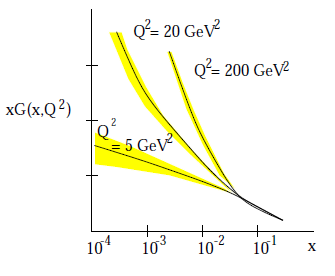
\includegraphics[width=0.5\textwidth]{HeraData}
    \caption{A representation of HERA deep inelastic scattering data, which shows
  	the accumulation of low-x partons from Reference~\cite{CGC2Lec}.}
    \label{HeraData}
  \end{figure}
  The CGC was inspired by and gives a natural explanation of deep inelastic
  	scattering data. 
  Figure~\ref{HeraData} gives a representation of the data collected by the HERA 
  	experiment. 
  The HERA data shows that as the constituents of a heavy ion are explored the
  	number constituents at lower momentum grows. 
  Following from right to left in Figure~\ref{HeraData} the gluon density
  	increases as $x$ decreases, where $x$ is the fraction of the total
  	momentum the constituent holds.
  The number of low momentum constituents can not however grow with out bound, a 
  	plateau must emerge.
  A plateau is required in order to assure unitarity, which requires that the
  	probability of scattering off the nucleus does not exceed one. 
  Emergence of a plateau would indicate evidence of saturation, the point where 
  	it becomes less favorable to produce more low momentum constituents. 
  As seen in Figure~\ref{HeraData}, the saturation scale increases as the momentum 
  	transfered to the probe $Q^2$ increases.
  This effect suggests that the saturation scale can be used to measure the 
  	running of the strong coupling constant predicted by standard
  	perturbative QCD.

  \section{Weizs\"{a}cker-Williams Approximation}
    The Weizsi\"{a}cker-Williams approximation relates the electric field of a 
      stationary point charge to the photon field that arises at ultra 
      relativistic velocities. 
    The approximation is semi-classical and combines both classical and quantum 
      elements.
    A Fourier transform of Maxwell's equations combine with Einstein's equation 
      for the energy of a photon in the Weizsi\"{a}cker-Williams approximation.
    \begin{wrapfigure}{r}{0.75\textwidth}
      \begin{center}
        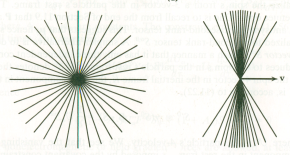
\includegraphics{boost.png}
      \end{center}
      \caption{ \label{fig:boost} The electromagnetic field boosted and at rest. }
    \end{wrapfigure}
    The frequency modes of the electrostatic field are treated as photons. 
    The conversion of the electric field to a flux of photons simplifies the
      calculation of interaction cross sections. 
    The Weizsi\"{a}cker-Williams approximation makes the calculation of 
      electromagnetic interactions with the nucleus tractable. 

    The Wiezacker-Williams approximation begins with the equation for the 
      electric field of the projectile nucleus at rest. 
    The electromagnetic field only needs to be considered at the position of 
      the target nucleus. 
    From the projectile's point of view, the target is moving and contributes
     $-vt$ to Eq.~\ref{eq:staticEFromTargtmp}, the equation for the electric 
     field of the projectile nucleus at rest.
    \begin{equation} \label{eq:staticEFromTargtmp}
        x'=-vt'\qquad
        y'=b\qquad
        z'=0\qquad
	\vec{\mathbf{E'}}=\left(\frac{eZ}
         {4 \pi \epsilon_{0}\left(\left(-vt'\right)^{2}+b^{2}\right)^{3/2}}\right)
	 \left(-vt'{\mathbf{\hat{x'}}+b\mathbf{\hat{y'}}}\right)
    \end{equation}        
    In Eq.~\ref{eq:staticEFromTargtmp}, $b$ is the impact parameter, 
      the distance of separation at closest approach, $v$ is the velocity of the 
      projectile nucleus, $Z$ is the number of protons in the nucleus, and $e$ 
      is the charge of the electron.
    Two simplifications occur due to the coordinates of 
      Eq.~\ref{eq:staticEFromTargtmp}.
    The magnetic field is equal to zero, because the projectile is at rest, and
      the $z$ coordinate can be ignored, reducing the equation to two dimensions. 

    The Lorentz transformation converts the field equations in the 
      projectile's frame to equations in the target's frame.
    The result is a set of equations that relate the electric and magnetic field
      components in one frame to the components of the electric and magnetic 
      field in another frame moving at a different constant velocity.
    Eq.~\ref{eq:staticEFromTarg2tmp} gives the result of the transformation 
      from the projectile's primed frame to the target's rest frame for 
      the field components \cite{WWJackson}:
    \begin{eqnarray} \label{eq:staticEFromTarg2tmp}
        E_{x}'=E_{x}\qquad
        \gamma\left(E_{y}'/c+\beta B_{z}'\right)=E_{y}/c\qquad
        \gamma\left(E_{z}'/c=\beta B_{y}'\right)=E_{z}/c \nonumber \\
        B_{x}'=B_{x}\qquad
        \gamma\left(B_{y}'-\beta E_{z}'/c\right)=B_{y}\qquad
        \gamma\left(B_{z}'+\beta E_{y}'/c\right)=B_{z}
    \end{eqnarray}
    The transformation equations for the fields, 
      Eq.~\ref{eq:staticEFromTarg2tmp}, and the transformation of the 
      coordinates reduce to Eq.~\ref{eq:staticEFromTarg3tmp} \cite{WWJackson}:
    \begin{eqnarray} \label{eq:staticEFromTarg3tmp}
        E_{x}'=E_{x}\qquad
        \gamma E_{y}'=E_{y}\qquad
        \gamma \beta E_{y}'/c=B_{z}\nonumber \\
        ct'=\gamma ct \qquad
        x'=-\gamma \beta c t
    \end{eqnarray}
    The simplicity of Eq.~\ref{eq:staticEFromTargtmp} creates the simplicity of
      Eq.~\ref{eq:staticEFromTarg2tmp}.
    The Lorentz transformation reduces the six components of the 
      electromagnetic field in the target's frame to the three equations in 
      Eq.~\ref{eq:staticEFromTarg2tmp} by relating them to the fields of the 
      projectile's frame. 
    
    The combination of Eq.~\ref{eq:staticEFromTargtmp} and 
      Eq.~\ref{eq:staticEFromTarg2tmp} produce equations for the electric and 
      magnetic fields in the target's rest frame. 
    Eq.~\ref{eq:staticEFromTargtmp} gives the expression for the field 
      components as seen in the projectile frame. 
    \begin{eqnarray} 
	\vec{\mathbf{E}}=\left( \frac{\gamma e Z}
         { 4 \pi \epsilon_{0} \left( \left( \gamma v t \right)^{2} 
	 + b^{2}\right)^{3/2} }\right)
         \left(vt\mathbf{\hat{x}}+b\mathbf{\hat{y}}\right)\qquad\nonumber \\
	 \vec{\mathbf{B}}=\frac{\gamma\beta e Z b}
	 { 4 \pi c \epsilon_{0} \left( \left( \gamma v t \right)^{2} 
	 + b^{2}\right)^{3/2} }
         \mathbf{\hat{z}}=
	 \frac{\gamma\mu_{0}veZb}{4\pi\left(\left(\gamma v t \right)^{2}
	 +b^{2}\right)^{3/2}}\mathbf{\hat{z}}
    \end{eqnarray}
    If the impact parameter $b$ goes to zero, the target sits in the line of 
      the projectile particle's motion, and the denominator carries a factor of
      $\gamma$ squared. 
    If $vt$ goes to zero, the projectile particle is directly above or below in
      the $y$ direction, and the numerator carries a factor of $\gamma$. 
    This results in fields that are a factor of $\gamma^3$ higher in the 
      $y$ direction than in the $x$ direction (see Fig.~\ref{fig:boost}).  
    The boost compresses the electric field of the charge 
      in the direction of the boost and produces a magnetic field 
      resulting in a form similar to radiation.
    The point charge at ultra relativistic velocities produces a strong 
      electric field in the plane transverse to its motion resembling a plane 
      wave.
         
    Separating the even and odd functions of the electromagnetic field simplify
      the decomposition of the field equations into Fourier modes.
    The even functions decompose into cosine functions, odd functions 
      into sine functions. 
    The y-component of the electric field and the z-component of 
      the magnetic field are even functions in time, and the 
      x-component of the electric field is an odd function in time.
    Eq.~\ref{eq:fourier1tmp} gives the Fourier transformation integrals. 
    \begin{eqnarray} \label{eq:fourier1tmp}
        E_{x}(\omega)=\sqrt{\frac{2}{\pi}}\frac{eZ}{4\pi\epsilon_{0}b^{2}}
         \int^{\infty}_{0}\frac{\left(\gamma vt/b\right)\sin
	 \left(\omega t\right)}
	 {\left(\left(\gamma vt/b\right)^{2}+1\right)^{3/2}}dt\qquad
	E_{y}(\omega)=\sqrt{\frac{2}{\pi}}\frac{\gamma eZ}
	 {4\pi\epsilon_{0}b^{2}} \int^{\infty}_{0}\frac{\cos(\omega t)}
	 {\left(\left(\gamma vt/b\right)^{2}+1\right)^{3/2}}dt\nonumber \\
	B_{z}(\omega)=\frac{\beta E_{y}(\omega)}{c}\qquad
    \end{eqnarray}
    With the appropriate substitutions, tables provide 
      solutions to the integrals of Eq.~\ref{eq:fourier1tmp} as seen in 
      Ref. \cite{WWFermi}.
    \begin{eqnarray}  \label{eq:fourier2tmp}
        u=\frac{\gamma v t}{b}\qquad du\left(\frac{b}{\gamma v}\right)=dt\qquad
	 \omega'=\frac{\omega b}{\gamma v}\nonumber \\
	\int^{\infty}_{0}\frac{u \sin(\omega'u)}{\left(u^{2}+1\right)^{3/2}}du
	 =\omega'K_{0}(\omega')\qquad
	\int^{\infty}_{0}\frac{\cos(\omega'u)}{\left(u^{2}+1\right)^{3/2}}
	 =\omega'K_{1}(\omega')
    \end{eqnarray}
    The Fourier transformation replaces the time variable with a frequency 
      variable in the field equations. 
    The frequency relates to photon energy by the Einstein's photon energy  
      equation, $E=\hbar\omega$.
    The substitution of time with frequency allows for a flux of photons 
      to replace the classical electromagnetic field.

    The $\gamma$ dependence of the field components is different because of the
      different $t$ dependence of Eq.~\ref{eq:fourier2tmp}.
    The integrals in Eq.~\ref{eq:fourier2tmp} shift the $\gamma$ dependence of 
      the field component equations.
    Eq.~\ref{eq:fourier3tmp} gives the result of the integrals:
    \begin{equation} \label{eq:fourier3tmp}
        E_{x}(\omega)=\sqrt{\frac{2}{\pi}}\frac{eZ}{4\pi\epsilon_{0}b^{2}}
	 \frac{b}{\gamma v}\frac{\omega b}{\gamma v}K_{0}
	 \left(\frac{\omega b}{\gamma v}\right)\qquad
	E_{y}(\omega)=\sqrt{\frac{2}{\pi}}\frac{\gamma eZ}{4\pi\epsilon_{0}b^{2}}
	 \frac{b}{\gamma v}\frac{\omega b}{\gamma v}K_{1}
	 \left(\frac{\omega b}{\gamma v}\right)\qquad
    \end{equation}
    $\gamma$ is subsumed into the substitution from $t$ to $\omega$ in the 
      numerator of the x-component and becomes a part of the zeroth-order 
      modified Bessel function upon integration.
    The y-component does not have a factor of $t$ in the numerator, therefore 
      the factor of $\gamma$ remains outside of the integral, and it does not 
      get subsumed into the first-order modified Bessel function.
    \begin{wrapfigure}{r}{0.5\textwidth}
      \begin{center}
        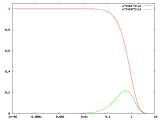
\includegraphics{bess.png}
      \end{center}
      \caption{\label{fig:bess} The zero and first order modified Bessel functions. }
    \end{wrapfigure}
    In Eq.~\ref{eq:fourier3tmp}, $E_{y}$ carries an additional factor of 
      $\gamma$ in the numerator relative to the $E_{x}$.
    $E_{y}$ is $\gamma$ times larger then $E_{x}$.

    In the ultra-relativistic limit, the electric and magnetic fields have the 
      same configuration as electromagnetic plane wave radiation. 
    The electric and magnetic fields are perpendicular and related by a factor
      of $c$ in the ultra relativistic limit.
    When $v$ approaches $c$, $\beta \approx 1$, the y-component of the 
      electric field and the z-component of the magnetic field are related by 
      a factor of $c$, $E_{y}/c=B_{z}$.
    Because $K_{0}(x)$ is smaller than $K_{1}(x)$ for all x, when $\gamma >> 1$, 
      $E_{y}$ is approximately equally to $\gamma$ $E_{x}$. 
    The conditions imposed by the ultra-relativistic limit result in the 
      relationship of Eq.~\ref{eq:ultraRelAprox}.
    \begin{equation} \label{eq:ultraRelAprox}
      \gamma >> 1 \rightarrow \gamma E_{x}>>E_{x} \rightarrow E_{y} >> E_{x}
    \end{equation}
    The x-component of the electric field can therefore be ignored and 
      the magnetic and electric fields are left perpendicular to each other.
    The six field components reduced to one electric component and one 
      perpendicular magnetic field component, which have a configuration 
      identical to a plane wave. 

    As with plane waves, the energy per area per time transfered by 
      the electromagnetic field is given by the Poynting vector.
    The Poynting vector takes the simple form of a plane pulse propagating in 
     the x direction.
    \begin{equation} \label{eq:poyntingVectortmp}
        \vec{\mathbf{S}}\equiv
	\vec{\mathbf{E}}\times\vec{\mathbf{B}}/\mu_{0}=
	\left(E_{y}^{2}/c\mu_{0}\right)\mathbf{\hat{x}}=
	c\epsilon_{0}E_{y}^{2}\mathbf{\hat{x}}
    \end{equation}
    The Poynting vector relates to the fluence (energy per unit area) 
      \cite{WWBrau},
    \begin{equation} \label{eq:fluencytmp}
        I(b)=\mathbf{\hat{x}}\cdot\int^{\infty}_{0}\vec{\mathbf{S}}d\omega=
	 \int^{\infty}_{0}\left(c\epsilon_{0}E_{y}^{2}\right)d\omega=
	 \int^{\infty}_{0}\left(\frac{dI}{d\omega}\right)d\omega
    \end{equation}
      and the spectral fluence (energy per area per frequency).
    \begin{equation} \label{eq:specturalFluencytmp}
	\frac{dI}{d\omega}=c\epsilon_{0}E_{y}^{2}=
	 \frac{e^{2}Z^{2}c}{4\pi^{3}b^{2}v^{2}\epsilon_{0}}
	 \left(\frac{\omega b}{\gamma v}\right)^{2}
	 K_{1}^{2}\left(\frac{\omega b}{\gamma v}\right)=
	\alpha\hbar\left(\frac{Z}{b\beta\pi}\right)^{2}
	 \left(\frac{\omega b}{\gamma v}\right)^{2}
	 K_{1}^{2}\left(\frac{\omega b}{\gamma v}\right)
    \end{equation}
    Substituting Eq.~\ref{eq:fourier3tmp} into Eq.~\ref{eq:fluencytmp} gives 
      the Poynting vector as a function of frequency.
    Eq.~\ref{eq:specturalFluencytmp} paves the way for Einstein's 
      equation. 
    The spectral fluence given by Eq.~\ref{eq:specturalFluencytmp} 
      relates the frequency to energy, which are the same quantities 
      present in Einstein's equation. 

    Einstein's equation, $E=\hbar\omega$, gives the energy of a photon, which
      is related to the spectral fluence. 
    If the fluence is due to a photon number density, $N$, Einstein's equation
      relates $N$ to the fluence. 
    The relationship between the number of photons per unit area in an 
      infinitesimal energy range and the spectral fluence in an infinitesimal 
      frequency range is given by Eq.~\ref{eq:photonFluxtmp} \cite{WWJackson}.
    \begin{equation}  \label{eq:photonFluxtmp}
        \frac{dI}{d\omega}d\omega=\hbar\omega N(\omega)d(\hbar\omega)
         \rightarrow \frac{1}{\hbar^{2}\omega}\frac{dI}{d\omega}=N(\omega)
    \end{equation}
    Plugging Eq.~\ref{eq:specturalFluencytmp} into 
      Eq.~\ref{eq:photonFluxtmp} yields the semiclassical photon flux of an 
      ultra-relativistic nucleus.
    \begin{equation} \label{eq:photonFluxFinaltmp}
	N(\omega,b)=\frac{\alpha}{\hbar\omega}
	 \left(\frac{Z}{b\beta\pi}\right)^{2}
	 \left(\frac{\omega b}{\gamma v}\right)^{2}
	 K_{1}^{2}\left(\frac{\omega b}{\gamma v}\right)
    \end{equation}
    Eq.~\ref{eq:photonFluxFinaltmp} replaces the classical electric field of a 
      point charge with a semiclassical field of photons. 
    Physicists can calculate the electromagnetic interactions between nuclei 
      with the final result of the Weizs\"{a}cker-Williams approximation, 
      Eq.~\ref{eq:photonFluxFinaltmp}.
    The photon flux in Eq.~\ref{eq:photonFluxFinaltmp} provides the 
      electromagnetic input to the $J/\psi$ photoproduction cross section 
      calculation. 


  \section{\label{sec:vdmTheory}Vector Meson Dominance}
    The Vector Messon Dominace method for calculating the $J/\psi$
      photoproduction cross section has three main components.
    VMD approach is constructed from the Weizsi\"{a}cker-Williams photon
      flux, the VMD fit to the proton-electron data, and the Glauber model for 
      calculating the nuclear cross sections from the proton-electron cross 
      sections.
    The Weizsi\"{a}cker-Williams photon flux provides the probe. 
    The proton-electron scattering data combine with the Glauber model  
      create a picture of the initial state of the nucleus. 
    Each of the different approaches to calculating the UPC $J/\psi$ 
      photoproduction cross section use these same elements.
    However, the different models each use the last two elements differently 
      to produce different pictures of the nucleus and different cross 
      sections values. 

    The photon flux in the photoproduction cross section calculation must be 
      finite in order for the cross section to be meaningful.
    The Weizsi\"{a}cker-Williams approximation, Eq.~\ref{eq:photonFluxFinaltmp}, 
      produces a divergence at $b=0$.
    The probability of the nuclei interacting would exceed one if the photon 
      flux were infinite. 
    The divergence that arises at $b=0$ from $K_{1}$ results in an 
      unphysically infinite photon flux.
    Removing the divergence is necessary.
    Special treatment of impact parameter, $b$, where the colliding nuclei 
      overlap eliminates the divergence. 
    
    A modulation of the photon flux can subdue the divergence at $b=0$.
    A convolution of the photon flux with the nucleon number density functions 
      of the colliding nuclei produces the necessary modulation. 
    Eq.~\ref{eq:woodsSaxon} gives the nucleon density of a single nucleus,
    \begin{equation} 
      \rho_{A}(s)=\frac{\rho_{0}}{1+exp[(s-R_{WS})/d)]}
      \label{eq:woodsSaxon}
    \end{equation}
    In Eq. ~\ref{eq:woodsSaxon}, $s$ is the distance from the center of the 
      nucleus, $R_{WS}$ is the radius of the nucleus, and $d$ is the skin depth, 
      which determines how quickly the nucleon density falls off beyond the 
      nuclear radius. 
    In Eq.~\ref{eq:TaNuc} the depth of the nucleus is integrated out leaving
      just the transverse dimension in $T_{A}$.
    The average number of nucleons in the overlap region is given by a 
      convolution of $T_A$ from each of the two nuclei to produce $T_{AA}$.
    \begin{eqnarray} \label{eq:TaNuc}
      T_{A}(\vec{r})=\int{dz\rho_{A}(\sqrt{|\vec{r}|^{2}+z^{2}})} \nonumber \\ 
      T_{AA}(|\vec{b}|)=\int{d^{2}\vec{r}T_{A}(\vec{r})T_{A}(\vec{r}-\vec{b})}
    \end{eqnarray}
    $T_{AA}$ is the function that modulates the photon flux. 
    As input to the Poisson distribution, $T_{AA}$ reduces 
      Eq.~\ref{eq:photonFluxFinaltmp} at values of $b$ where the nuclei overlap 
      significantly and eliminates the divergence in the photon flux. 
    
    Modulating the photon flux by the probability that no nucleon-nucleon 
      collisions occur limits the photon flux at low $b$ in Eq.~\ref{eq:photonFluxFinaltmp}.
    The convolution of the photon flux with the $b$ dependent probability that 
      no nucleon-nucleon collisions occur removes the divergence in 
      Eq.~\ref{eq:photonFluxFinaltmp}. 
    Using the mean number of nucleons in the overlap region given by $T_{AA}$, 
      the Poisson distribution gives the probability that no collisions 
      occur at a given $b$:
    \begin{equation} \label{eg:poisNoCol}
      P_{0}(b)=exp[-T_{AA}(b)\sigma_{NN}]
    \end{equation}
    In Eq.~\ref{eg:poisNoCol}, $\sigma_{NN}$ is the cross section for a 
      nucleon-nucleon interaction, which gives the probability that a collision
      will occur given the average number of nucleons in the overlap region.
    The average photon flux over impact parameter, $b$, can be calculated 
      from the integration of the $b$-dependent photon flux, Eq.~\ref{eq:photonFluxFinaltmp}, 
      with the $b$-dependent probability of having no nucleon-nucleon 
      interactions, Eq.~\ref{eg:poisNoCol}. 
    \begin{equation} \label{eq:fluxMod}
      \frac{dN_{\gamma}(k)}{dk}=\int_{0}^{\infty}{2\pi bdbP_{0}(b)
         \int_{0}^{R}{\frac{rdr}{\pi R^{2}_{A}}\int_{0}^{2\pi}d\phi
         \frac{d^{3}N_{\gamma}(k,b+r\cos(\phi))}{dkd^{2}r}}}
    \end{equation}
    Eq.~\ref{eq:fluxMod} goes down to $b=0$ where the photon flux is infinite, but 
      because the probability of having a nucleon-nucleon collisions is high, 
      the divergence is eliminated.
    The result of Eq.~\ref{eq:fluxMod} does not diverge.  

    A power-law fit to the proton photoproduction data gives an analytic 
      expression for the energy dependence of the proton photoproduction 
      cross section.
    The fitting function is simple and only depends on the photon-proton center
      of mass energy, $W$. 
    Eq.~\ref{eq:proElFit} gives the parameterization of the forward 
      proton photoproduction cross section fit. 
    \begin{equation} \label{eq:proElFit}
      \frac{d\sigma(\gamma p\rightarrow Vp)}{dt}\Big|_{t=0}
        =b_{v}(XW^{\epsilon}+YW^{-\eta})
    \end{equation}
    $W$ is the center of mass energy of the proton-photon system in 
      Eq.~\ref{eq:proElFit}.
    The remaining variables in Eq.~\ref{eq:proElFit} are simple power-law fit
      parameters.  
    The $XW^{\epsilon}$ term characterizes pomeron mediated interactions, and
      the $YW^{\eta}$ term characterizes meson mediated interactions\cite{vmd1999}. 
    $J/\psi$'s high mass relative to the $\pi$ and $\rho$ renders the second 
      term in Eq. ~\ref{eq:proElFit} negligible as the term falls rapidly with
      increasing $W$. 
    Eq.~\ref{eq:proElFit} allows for extrapolation and interpolation of the 
      measured forward proton photoproduction cross section. 
    The fit to the data provides estimates for energies that have not yet been 
      probed experimentally.

    The proton-electron scattering data is used differently in the VMD method 
      than in the other major methods.  
    The VMD method for calculating UPC photoproduction cross sections 
      relies more on electron-proton scattering data.
    The proton photoproduction cross sections from the electron-proton 
      scattering data is a direct input to the VMD model. 
    A power-law fit to the proton photoproduction data, as opposed to model 
      dependent gluon densities of other approaches, combines with the Glauber
      model to provide the nuclear model in the VMD method. 
    Because of the simplicity of the method, the VMD approach incorporates less
      modifications of the nuclear initial state relative to the proton initial
      state. 
    As a result, the VMD method produces a higher UPC J/$\psi$ photoproduction 
      cross section relative to the other methods. 

    Vector meson dominance and the optical theorem allow for the calculation of 
      the total proton-meson scattering cross section from the fit given by 
      Eq.~\ref{eq:proElFit}. 
    The optical theorem relates a total cross section, $\sigma$, 
      to a corresponding forward scattering cross section, $d\sigma/dt|_{t=0}$.
    Vector meson dominance asserts that the colored part of the photon wave 
      function is dominated by vector mesons; therefore, the photon is 
      represented as a quark-antiquark pair in photoproduction calculations. 
    These two components combine to produce Eq.~\ref{eq:VMDforwardScat}.
    \begin{eqnarray} \label{eq:VMDforwardScat}
      \frac{d\sigma(\gamma p\rightarrow Vp)}{dt}\Big|_{t=0}=
        \frac{4\pi \alpha}{f^{2}_{v}(M_{V},\Gamma_{l^{+}l^{-}})}\frac{d\sigma(Vp\rightarrow Vp)}{dt}
        \Big|_{t=0} \nonumber \\
       \sigma(Vp)_{tot}^{2}=16\pi\frac{d\sigma(Vp\rightarrow Vp)}{dt}\Big|_{t=0}
    \end{eqnarray}
    In Eq.~\ref{eq:VMDforwardScat}, the photon-proton scattering is related to
      meson-proton scattering through the photon-meson coupling, which 
      depends on the vector meson's mass, $M_{V}$, and leptonic decay width, 
      $\Gamma_{l^{+}l^{-}}$. 
    The result of combining vector meson dominance and the optical theorem 
      in Eq.\ref{eq:VMDforwardScat} provides the cross section for a meson to 
      scatter off a proton.
    The total proton-meson scattering cross section, provides 
      the input to the Glauber model calculation of the nuclear photoproduction 
      cross section. 

    The nucleus-meson scattering cross section relates to 
      Eq.~\ref{eq:VMDforwardScat} through the Glauber model. 
    The Glauber model allows for Eq.~\ref{eq:VMDforwardScat}, the proton-meson
      scattering cross section, to be used to calculate a nucleus-meson 
      scattering cross section. 
    The Glauber model produces nuclear cross section calculations from 
      nucleon (proton or neutron) interaction cross sections by use of $T_{AA}$. 
    The combination of the mean number of nucleons in the overlapping region
      of a nucleus-nucleus collision, $T_{AA}$, the nucleon cross section, 
      $\sigma$, and the Poisson distribution make-up the core of the Glauber 
      model. 
    For the total nucleus-meson scattering cross section, the equation has the 
      following form:
    \begin{equation} \label{eq:glauber}
      \sigma_{tot}(VA)=\int d^{2}\vec{r}(1-e^{-\sigma_{tot}(Vp)T_{AA}(\vec{r})})
    \end{equation}
    In Eq.~\ref{eq:glauber}, the term $e^{\sigma_{tot}(Vp)T_{AA}}$ gives the
      probability of having no meson-nucleon scatterings from the Poisson 
      distribution. 
    The probability of having at least one scattering is given by subtracting 
      one from the term  $e^{\sigma_{tot}(Vp)T_{AA}}$ in Eq.~\ref{eq:glauber}.
    As seen in Eq.~\ref{eq:glauber}, the Glabuer model leverages scientific 
      knowledge of the proton to understand of the nucleus. 
    The Glauber model is the tool that combines the proton photoproduction data 
      with nucleon distributions in the nucleus to produce a nuclear vector 
      meson photoproduction cross section in the VMD approach. 

    Reversing the process used for the proton, Eq.~\ref{eq:glauber}, the meson 
      nucleus scattering cross section, relates to forward nuclear 
      photoproduction cross section through the optical theorem. 
    The nuclear photoproduction cross section is the input to the calculation 
      of the final result, the nuclear vector meson photoproduction cross 
      section in UPC events.  
    Eq.~\ref{eq:optTheA} uses the optical theorem to produce the nuclear 
      photoproduction cross section from the nucleus-meson scattering cross 
      section:
    \begin{eqnarray} \label{eq:optTheA}
      \frac{d\sigma(\gamma A\rightarrow VA)}{dt}\Big|_{t=0}=
      \frac{\alpha\sigma_{tot}^{2}(VA)}{4\pi f_{v}^{2}}\nonumber \\
      \sigma(\gamma A\rightarrow VA)=\frac{d\sigma(\gamma A\rightarrow VA)}{dt}
        \Big|_{t=0}\int_{t_{min}}^{\infty}dt|F(t)|^{2}
    \end{eqnarray}
    $F$ in equation Eq.~\ref{eq:optTheA} is the Fourier transform of the 
      nuclear density function, $\rho_{A}$.
    To produce the formula for calculating the UPC vector meson 
      photoproduction cross section, Eq.~\ref{eq:optTheA} is combined with the 
      photon flux incident on the nucleus, Eq.~\ref{eq:fluxMod}. 
    \begin{equation} \label{eq:finalVMDResult}
      \sigma(AA\rightarrow AAV)=2\int{dk\frac{dN_{\gamma}}{dk}
                    \sigma(\gamma A\rightarrow VA)}
    \end{equation}
    The factor of 2 in Eq.~\ref{eq:finalVMDResult} comes from the fact that both 
      of the two colliding nuclei contribute. 
    Combining the three elements of VMD, Eq.~\ref{eq:finalVMDResult} is the 
      final result of the VMD UPC photoproduction cross section calculation. 
    Vector meson production rates in UPC collisions are predicted 
      by Eq.~\ref{eq:finalVMDResult}, which can be confirmed or denied by 
      experiment. 


      \section{\label{sec:ltaTheory}Leading Twist Approach Derivation}
    The LTA method for calculating UPC photoproduction cross sections
      combines elements of the Glauber model with direct use of gluon 
      densities. 
    The proton gluon density is modified by a nuclear modification 
      function in the LTA method to produce the nuclear gluon density. 
    The nuclear modification function converts the proton photoproduction
      cross section to a nuclear photoproduction cross section in the LTA 
      method.
    The LTA method is different from the other methods in its direct use of the
       nuclear modification factor and how the nuclear modification factor
       calculation incorporates multiple scattering.
    The direct use of the nuclear modification factor produces the most gluon 
      shadowing out of the three major methods, and results in the lowest
      cross sections.
    The LTA method is the easiest to constrain experimentally for this reason. 

    The LTA method uses the Weizsi\"{a}cker-Williams approximation to calculate 
      the photon flux created by the colliding nuclei. 
    As in the VMD method, the probability of having no hadronic collisions 
      modulates the flux.
    The photon flux for the LTA method has the following form \cite{lta2011.09}:
    \begin{eqnarray} \label{eq:ltaPhotonFlux}
      n_{\gamma/A}^{i}(\omega_{\gamma})=\frac{2\alpha Z^{2}}{\pi}\int_{b_{min}}^{\infty}
        db\frac{x^{2}}{b}\Big[K_{1}^{2}(x)+\frac{K_{0}^{2}(x)}{\gamma_{L}^{2}}\Big]
        P_{0}(b)P_{C}^{i}(b) \\
      x=\frac{\omega b}{\gamma_{L} v} \nonumber 
    \end{eqnarray}
    The $K_{0}^{2}(x)$ term contributes a photon flux in the 
      transverse direction.
    $P_{C}^{i}(b)$ is an additional modulation factor that requires various 
      additional interactions. 
    These interactions result in additional emissions of neutrons from the 
      receding nuclei as the nuclei relax from excited states. 
    The LTA flux reproduces the VMD result when the $K_{0}$ term becomes 
      negligible as $\gamma_{L}$ approaches $\infty$ and $P_{C}^{i}=1$ when all
      emissions are allowed.
    The terms $P_{C}^{i}$ and $K_{0}$ create additional ways to distinguish UPC
      events from nuclear collisions experimentally but leave the underlying 
      interaction mechanism the same. 
    For example, the additional terms in the LTA formulation of the photon flux
      produce calculations of asymmetric neutron emission, which separate UPC 
      events from nuclear collisions.  

    The LTA method calculates the nucleon photoproduction cross section 
      from the nucleon gluon density. 
    Ref. \cite{lta2011.09} derives the nucleon cross section from derivations
     of the nucleon gluon densities from electron-proton scattering data and
     leading order perturbative quantum field theory calculations.
    The forward photoproduction cross section of the nucleon has the following
     form \cite{lta2011.09}:
   \begin{equation} \label{eq:ltaFowardPhotoXSec}
     \frac{d\sigma_{\gamma N\rightarrow J/\psi N}(t=0)}{dt}=\frac{16\Gamma_{l^{+}l^{-}}\pi^{3}}
     {3\alpha M_{J/\psi}^{5}}[\alpha_{s}\mu^{2}xG_{N}(x,\mu^{2})]^{2}
   \end{equation}
   Here $G_{N}$ is the gluon density of the nucleon, $x$ is the fraction of
     the nucleon's momentum the gluon carries, and $\mu$ is related
     to momentum at which the nucleon is being probed, which is equal to 
     $M_{J/\psi}/2$ for $J/\psi$ photoproduction.
   In Eq.~\ref{eq:ltaFowardPhotoXSec} the nucleon cross section is explicitly 
     connected to the gluon density.
   By connecting the gluon density to the cross section, Eq.~\ref{eq:ltaFowardPhotoXSec}
     allows for the gluon density to be experimentally probed. 

   Ref. \cite{lta2011.09} exploits the optical theorem to relate the forward 
     photoproduction cross section of the nucleon to the nuclear cross section. 
   Eq.~\ref{eq:ltaOptTheWNucMo} gives the relation:
   \begin{eqnarray} \label{eq:ltaOptTheWNucMo}
     \sigma_{\gamma A\rightarrow J/\psi A}(\omega)=
     \frac{d\sigma_{\gamma N\rightarrow J/\psi N}}{dt}(\omega,t_{min})
     R_{g}^{2}\int_{t_{min}}^{\infty}dt|F(t)|^{2} \\
     R_{g}=\frac{G_{A}(x,\mu^{2})}{AG_{N}(x,\mu^{2})} \nonumber 
   \end{eqnarray} 
   $R_{g}$, the nuclear modification function, is the ratio between the gluon 
     density of the nucleon, $G_{N}$, to the gluon density of the nucleus, 
     $G_{A}$.
   As with the VMD method, the optical theorem relates the forward cross 
     section, $\frac{d\sigma_{\gamma N\rightarrow J/\psi N}}{dt}(\omega,t_{min})$,
     to the total cross section, $\sigma_{\gamma A\rightarrow J/\psi A}$. 
   The LTA method relates the measurable UPC photoproduction cross section 
     to the gluon density of the nucleus.  
   Eq.~\ref{eq:ltaOptTheWNucMo} further connects the gluon density of the 
     nucleon to the relative reduction of the gluon density in the nucleus 
     through $R_{g}$.

   From Eq.~\ref{eq:ltaOptTheWNucMo}, the LTA method can predict the angular 
     distribution of photoproduced $J/\psi$ with respect to the beam axis. 
   In Ref. \cite{lta2012.03} the angular distribution is expressed in the form 
     of the rapidity dependency of the UPC photoproduction cross section. 
   \begin{eqnarray} \label{eq:ltaRapDist}
     \frac{d\sigma_{A_{1}A_{2}\rightarrow A_{1}A_{2}J/\psi}}{dy}=
       n_{\gamma/A_{1}}(y)\sigma_{\gamma A_{2}\rightarrow J/\psi A_{2}}(y)
       +n_{\gamma/A_{2}}(-y)\sigma_{\gamma A_{1}\rightarrow J/\psi A_{1}}(-y) \\
       y=ln\Big(\frac{2\omega}{M_{J/\psi}}\Big) \nonumber
   \end{eqnarray}
   Eq.~\ref{eq:ltaRapDist} is comprised of two terms, one for photons from the
     forward going nucleus interacting with the backward going nucleus, and 
     a second for the reverse situation. 
   The integration of Eq.~\ref{eq:ltaRapDist} over $y$ produces the factor of 2 
     that is present in Eq.~\ref{eq:finalVMDResult}.
   The rapidity distribution of the photoproduction cross section given in 
     Eq.~\ref{eq:ltaRapDist} provides a more detailed prediction and allows for
     more direct experimental comparison.
   Eq.~\ref{eq:ltaRapDist} allows for comparison to rapidity regions that are 
     covered by experiments.
  
   The LTA method is distinct from the pQCD method and VMD method through the 
     use $R_{g}$, the nuclear gluon modification factor. 
   As opposed to using $R_{g}$, the pQCD method uses the nuclear gluon 
     density, and VMD model uses proton photoproduction cross sections 
     directly. 
   In the LTA method, $R_{g}$ is calculated through a combination of $J/\psi$ 
     photoproduction data from proton-electron scattering and DGLAP evolution 
     equations, which incorporates nuclear multiple scattering effects 
     \cite{lta2011.09}. 
   The DGLAP evolution equations give the depends of nuclear gluon densities on
     the momentum scale at which the nucleus is probed, $\mu$ in 
     Eq.~\ref{eq:ltaFowardPhotoXSec}. 
   The unique way the LTA method calculates $R_{g}$ results in lower cross 
     sections than the other major methods and allows for experimental
     sensitivity. 
   Experimental measurements of the UPC $J/\psi$ photoprodcution cross section 
     with CMS have the opportunity to distinguish whether $R_{g}$ as calculated 
     in the LTA method accurately predicts the gluon density of the nucleus. 
  
 
  \section{Perturbative Quantum Chromo-dynamics}
    To calculate the UPC $J/\psi$ photoproduction cross section, the pQCD 
      method uses the nuclear gluon density to characterize the nucleus and 
      the Weizs\"{a}cker-Williams approximation for the probing photon flux. 
    The pQCD method combines these components such that the nuclear gluon 
      density is a direct variable.
    The nuclear gluon density term in the pQCD formulation allows for 
      the use of a variety of nuclear gluon density models.
    A range of nuclear gluon densities are present in the available models
      resulting in a wide range of cross section values. 
    The UPC $J/\psi$ photoproduction cross section is correlated with the gluon
      density of the nucleus rising with higher densities and shrinking with 
      lower densities. 
    In the pQCD approach, the calculation of the UPC $J/\psi$ photoproduction 
      cross section allows experiments to constrain many different nuclear 
      gluon density models. 
    
    In the pQCD method, the photon interacts with the nucleus by fluctuating to 
      a quark-anitquark pair.
    For $J/\psi$, the photon fluctuates to a $c\bar{c}$ pair. 
    The probability for the photon to fluctuate to a $c\bar{c}$ pair
      depends on the $M_{J/\psi}$, the mass of $J/\psi$, $\Gamma_{l^{+}l^{-}}$, 
      the $J/\psi$ leptonic decay width, and $\alpha$, the electromagnetic 
      coupling constant.
    These three variables connect the c quark to the electromagnetic force 
      mediator, the photon. 
    Recast as a $c\bar{c}$ pair, the photon couples to the nuclear gluon 
      density.
    Ref. \cite{pQCD2011.08} uses the fluctuation of the photon to a $c\bar{c}$ 
      pair as the foundation for calculating the forward $J/\psi$ 
      photoproduction cross section. 

    The $c\bar{c}$ pair arising from the photon fluctuation scatters off the 
      gluons of the nucleus. 
    The density of gluons in the nucleus determines how likely and therefore 
      how large the cross section is for the quarks to scatter and form a 
      $J/\psi$.
    The forward scattering cross section is the portion of those scattering 
      events which transfer the minimum amount of momentum between the 
      photon and the nucleus. 
    The forward cross section for $J/\psi$ photoproduction in the nucleus has 
      the following form \cite{pQCD2011.08}:
    \begin{equation} \label{eq:pQCDfowardScat}
      \frac{d\sigma_{\gamma A\rightarrow J/\psi A}}{dt}\Big|_{t=0}=\xi_{J/\psi}
        \Big(\frac{16\pi^{3}\alpha_{s}^{2}\Gamma_{l^{+}l^{-}}}{3\alpha 
        M_{J/\psi}^{5}}\Big)[xG_{A}(x,\mu^{2})]^{2}
    \end{equation}
    In Eq.~\ref{eq:pQCDfowardScat}, $\xi_{J/\psi}$ is an experimentally derived 
      correction factor, $\alpha_{s}$ is the strong coupling constant, $x$ is 
      the momentum faction of the nucleus the scattering gluons carry, and 
      $G_{A}$ is the gluon density of the nucleus. 
    Both the $c$ and $\bar{c}$ couple to the gluon density, and the double 
      coupling results in the squared dependence of the cross section on the 
      gluon density in Eq.~\ref{eq:pQCDfowardScat}. 
    Fitting Eq.~\ref{eq:pQCDfowardScat} to proton-electron scattering data 
      sets $\xi_{J/\psi}$ \cite{pQCD2011.08}.
    The forward scattering cross section given by Eq.~\ref{eq:pQCDfowardScat} 
      connects the photon flux to the gluon density and provides the input to 
      calculate the total cross section by the optical theorem. 
    Eq.~\ref{eq:pQCDfowardScat} is the crux of how UPC measurements provide
      insight into the gluon content of the nucleus.
    
    The optical theorem relates the forward cross section in 
      Eq.~\ref{eq:pQCDfowardScat} to the total photoproduction cross section. 
    The total cross section calculated by use of the optical theorem gives 
      the probability that a photon incident on the nucleus will produce a 
      $J/\psi$ regardless of the momentum transfered in the interaction. 
    Ref. \cite{pQCD2011.08} gives the form of the total cross section equation:
    \begin{equation} \label{eq:pQCDtotXSec}
      \sigma_{\gamma A\rightarrow J/\psi A}(k)=
      \frac{d\sigma_{\gamma A\rightarrow J/\psi A}}{dt}\Big|_{t=0}
      \int_{t_{min}(k)}^{\infty}dt|F(t)|^{2}
    \end{equation} 
    Here $t_{min}=(M_{J/\psi}^{2}/4k\gamma_{L})^2$, which is the minimum amount
      of momentum transfer required to produce a $J/\psi$ given the photon wave
      number $k$.
    The $k$ dependence of $t_{min}$ produces the rapidity, $y$, dependence of
      the total cross section.
    The total cross section for photoproduction, Eq.~\ref{eq:pQCDtotXSec}, 
      provides the input to Eq.~\ref{eq:ltaRapDist}, 
      which gives the rapidity dependence of the UPC photoproduction cross 
      section. 
    Eq.~\ref{eq:pQCDtotXSec} as input to Eq.~\ref{eq:ltaRapDist} allows for 
      experimental comparison of the pQCD method to measurements of UPC 
      photoproduction cross sections. 
    With the pQCD method's direct use of the nuclear gluon density in 
      Eq.~\ref{eq:pQCDfowardScat}, the pQCD method allows for experimental 
      exploration of any gluon density model. 


  \section{Incoherent Photoproduction}


  \section{Photon Induced Nuclear Break-up}
    Two different approaches are discussed.
    The first is to measure the desired cross-section directly.
    This can be done by bombarding the target material with mono-energetic real photons, varying the energies of the photons over a range of frequencies, and extrapolating that data up to the photon energies that arise in the Weizäcker-Williams approximation [3].
    The other approach is to create a theoretical model of how the target reacts to a photon flux [4].
    In the theoretical model that will be discussed in this paper, the photonuclear cross-section, the cross-section governing the absorption of photons by a nucleus, is formulated as the sum of two other cross-sections that are known better.
    In both, the more detailed theoretical approach and the empirical approach to the problem, the interaction of the Weizäcker-Williams quasi-real photons is assumed to be identical to the interaction of real photons with the target.

    To model the interaction of the photons with the target nuclei, as done in Ref.
    [4], the photonuclear cross-section is broken down into two parts.
    
    (16)
    The Giant Dipole Resonance (GDR) cross-section dominates at lower photon frequencies and is the result of the collective motion of the protons relative to the neutrons.
    The Quasi-Deuterium (QD) cross-section dominates at higher photon energies and is the result of treating the nucleus as a collection of proton-neutron pairs, which is deuterium.

    The giant dipole resonance has been studied for decades.
    In 1947, Baldwin and Klaiber first observed the giant dipole resonance [6].
    At the General Electric Research Laboratory, Baldwin and Klaiber found that by bombarding a uranium target with photons in the range 10 – 100 MeV, a peak in the spectrum was found for photons at 20 MeV.
    A year later, Goldhaber and Teller theorized that this was the result of the protons moving back and forth with respect to the neutrons [6].
    In this model, the protons and neutrons are treated as two separate liquid dots.
    Then in 1950, Steinwedel and Jensen modified this theory by modeling the protons and neutrons as fluids contained in a single sphere rather than two separate dots moving back and forth [6].
    
    In order to understand the Goldhaber and Teller model, it is useful to consider a nucleus where the number of protons and neutrons are equal, Z=A/2.
    The collection of protons and the collection of neutrons move opposite each other and only in the z direction.
    In order to construct a Hamiltonian, first the kinetic energy should be considered.
    
    (17)
    Eq.
    17 is the familiar equation for kinetic energy simply summed over all the constituent nucleons of the nucleus.
    The protons and neutrons are modeled as separate liquid drops with densities $\rho$p and  $\rho$n.
    These liquid dots will oscillate back and forth in opposite phase relative to the center of mass maintaining there individual density profiles.
    
    The potential holding protons and neutrons together depends on the difference of the two densities squared.
    If the two exactly overlap, there is no difference in the densities and the potential energy is zero.
    If the two density distributions are separated, there will be regions where the neutron density is greater and regions where the proton density is greater.
    In the separated configuration, there will be potential energy.
    The potential energy can be shown to have the form of a harmonic oscillator with a spring constant that depends on the initial density distribution [6].

    (18)
    If the nucleus has a shape cut off in density at it's very edge, then the integral is dominated  by the region at the surface, and the spring constant K becomes proportional to the mass number to the 2/3rds power, A2/3.
    This is the consequence of the of geometry of a sphere.
    The surface area of a sphere is proportional to its volume to the 2/3rds power.
    Recalling the angular frequency of a harmonic oscillator,
    (19)
    it is seen that the frequency of the giant dipole resonance in the Goldhaber and Teller model is proportional to the mass number to the negative 1/6th power, A-1/6.
    This dependence describes light nuclei well, but it does not describe heavier nuclei [6].

    In order to describe heavier nuclei, the Steinwedel and Jensen model must be used.
    In the  Steinwedel and Jensen model, the proton and neutron fluids are confined to a single sphere where they are allowed to slosh back and forth creating the same effect as the Goldhaber and Teller model.
    In this model, there is no global separation of the proton and neutron fluids.
    The dipole is created by underdensities and overdensities of the proton and neutron fluids.
    It can be shown that this results in a frequency of oscillation which depends on one over the radius of the nucleus [6]:
    (20)
    As before, the relationship in Eq.
    20 arises from the geometry of a sphere.
    The dependence of the giant dipole resonance that is seen in the Steinwedel and Jensen describes medium and heavier mass nuclei well.
    Empirically, both models are stitched together to give the following mass number dependence of the peak dipole resonance [6].

    (21)
    In order to compute the effect of an excitation in either model, the harmonic oscillator solutions found earlier can be driven by an interacting force.
    The resulting differential equation can then be solved using a Fourier transform to eliminate the time derivatives and reduce the equation to an algebraic equation.
    Following this procedure produces the shape of energy dependence of the giant dipole resonance, and this gives a cross-section for photon absorption by the giant dipole resonance with Lorentzian form [6]:
    (22)
    here $\sigma$max is the maximum cross-section, when E$\gamma$g = EGDR, EGDR is the peak resonance energy, and $\Gamma$GDR is the width of the resonance.
    The width, $\Gamma$GDR, of this distribution lies in a range from 4-8 MeV and depends on the orbital arrangement to the neutrons and protons in the given nucleus [6].
    
    For higher energy photons, the quasi-deuterium cross-section is needed.
    The quasi-deuterium approach amounts to treating the nucleus as a bunch of proton-neutron pairs, which are screened by the rest of the nucleus.
    Eq.
    23 models this behavior [4].
    
    (23)
    Here $\sigma$d is the deuterium disintegration cross-section for $\gamma$g+d $\rightarrow$ p+n.
    F is a function that arising from Pauli blocking of fermions, and L is an empirical parameter set by data that is equal to 6.5.
    Certain energy levels are not available to the products of the deuterium disintegration process because of the presence of the rest of the nucleus.
    The result is a reduction of the cross-section.
    
    F can be modeled with an exponential cutoff below 20 MeV, a polynomial in the intermediate range with nearly linear dependence on E$\gamma$g, and above 140 MeV an inverted exponential pushing F to one at higher values of E$\gamma$g [4].
    Essentially, the model at low photon energies disallows deuterium disintegration because the products have no available state to occupy, and at high energies the rest of the nucleus becomes transparent and looks more and more like a collection of deuterium.
    The deuterium disintegration cross-section is found empirically and is fit to the following function [4]:
    (24)
    In order to produce a final state for the target nucleus, a branching ratio is needed.
    The branching ratio gives the probability that the photo-excited nucleus will end up in a particular state.
    This determines the sort of emission that will result from the de-excitation process.
    There are two phases of deexcitation, the nonequlibrium phase and the equilibrium phase.
    In the time before reaching equilibrium, fast nucleons are emitted.
    Subsequently, in the equilibrium phase, slow nucleons evaporate.
    These two phases are simulated in complex computer codes that calculate branching ratios (see discussion in Ref.
    [4]).

    All the tools are now assembled to calculate the cross-section for any particular electromagnetic dissociation process.
    The first step in the calculation is to assume that the number of photons absorbed by either nucleus in the collision obeys the Poisson distribution [3,4].
    An average number of absorptions is calculated and used in the construction of the distribution.

    (25)
    When using the model of Ref.
    [4], the cross-section involved in Eq.
    25 will be the photonuclear cross-section, and the calculation will produce the average number of photons absorbed by the target.
    If instead the empirically measured photoneutron cross-section is used as in Ref.
    [3], the mean calculated in Eq.
    25 will be the number of photons absorbed that result in neutron emission from the target.
    This restricts the calculation to only de-excitation modes that produce neutrons.
    Both averages are for a given impact parameter b.

    Following Ref.
    [3] and using the experimentally measured photoneutron cross-section, the probability Pn for the target to produce a number of neutrons, k, due to the photon flux of the projectile can be calculated using Eq.
    26.

    (26)
    This is just the Poisson distribution.
    In the collider situation, where both nuclei can be treated as the target and the projectile, the probability of mutual emission, one nucleus emitting x neutrons and the other emitting y neutrons, can be calculated from Eq 27.

    (27)
    It is also interesting to consider the situation where at least one neutron is emitted.
    This can be calculated by subtracting the probability of no neutrons being emitted from one.

    When using the model of Ref.
    [4], a branching ratio is needed to calculate the probability of de-exciting into a given state.
    The probability of photon absorption is calculated as in Eq.
    26, only using the model of Ref.
    [4].
    This is the probability of the target absorbing k photons rather than then the nucleus absorbing a photon and emitting a neutron.
    In Ref.
    [4], the probability of any final state i due to the absorption of a single photon can be calculated using Eq.
    28.

    (28)
    Here Pa is the probability that the target absorbs a single photon as calculated by Eq.
    26, q is the probability that the photon will have the frequency $\omega$, and fi is the branching ratio.
    The following equation describes q [5].

    (29)
    By multiplying Eq.
    26 and 29 in Eq.
    28, the m(b) terms cancel and produce a simplified equation.
    The forms for probability functions, like Eq.
    28, that involve absorption of multiple photons have additional terms.
    But they follow that same scheme of multiplying the probability of absorption times the probability that the absorbed photon has a particular frequency times the branching ratio.

    The probability functions Eq.
    26 and Eq.
    28 can than be used to produce cross-sections.
    For any given process, using Eq.
    28 can be used by inserting the appropriate branching ratio.
    For emission of neutrons, Eq.
    26 can be used.
    This is done by integrating over the impact parameter to get an area that is weighted by the probability functions [3,4].

    (30)
    If the branching ratio for neutron emission is selected in Eq.
    28, then Eq.
    28 and Eq.
    26 can be used to compute the same cross-section through the use of Eq.
    30.
    
    Three parameters arise when calculating the cross-section in Eq.
    30, the minimum impact parameter bo, the minimum emitted photon frequency $\omega$min, and the maximum emitted photon frequency $\omega$max.
    The need for a minimum impact parameter is necessitated by the Bessel function in the photon flux in Eq.
    14.
    At zero, the modified Bessel function does not converge.
    Physically, a minimum impact parameter is selected in order to separate the domains between electromagnetic interactions and the strong interactions that happen inside the nucleus.
    To serve this end, the minimum impact parameter is set to the radius of the nuclei [3,4].
    This excludes collisions where the nuclei overlap in the calculation, and assures only electromagnetic interactions are involved.

  \section{Theoretical Results}
  The UPC photoproduction cross section calculations depend significantly on 
    how the nucleus is represented in the calculation. 
  The results from the VMD, LTA, and pQCD methods vary from a relatively 
    large cross section in the VMD model, ranging through a variety of values
    in the pQCD method, to a relatively small cross section in the LTA method. 
  Each of these methods utilizes the same probe of the nucleus, the equivalent 
    photon flux that is calculated using the Weizsi\"{a}cker-Williams approximation. 
  The three methods deviate in how they calculate the forward photoproduction
    scattering cross section.
  The differences in the UPC photoproduction cross sections predicted by the 
    different models demonstrates the amount of experimental sensitivity there 
    is to distinguishing between the models. 
  The dependence of the cross section on rapidity shows where in phase space 
    a measurement of the cross section is most sensitive.
   
  The predicted value for the UPC $J/\psi$ photoproduction cross section in 
    PbPb collisions at the LHC differ widely depending on which of the three 
    main methods is used. 
  The cross section value calculated by Eq.~\ref{eq:finalVMDResult} in the 
    VMD, LTA, and the various gluon density models in pQCD method vary 
    significantly.
  Table~\ref{tab:allXsec} gives the predicted values for the three main methods
    taken from Ref~\cite{pQCD2013.02}, Ref~\cite{lta2011.09}, and Ref~\cite{vmd1999}.
  \begin{table} 
   \centering
   \begin{tabular}{|l|l|} 
     \hline
     Model & $\sigma_{AA\rightarrow AAJ/\psi} (mb)$ \\ \hline \hline
     VMD/STARlight MC & 23 \\ \hline
     LTA & 9 \\ \hline
     pQCD-MSTW08 & 34 \\ \hline
     pQCD-EPS08 & 7  \\ \hline
     pQCD-EPS09 & 14 \\ \hline
     pQCD-HKN07 & 23 \\ \hline
     \hline
   \end{tabular}
   \caption{$\sigma_{AA\rightarrow AAJ/\psi} (mb)$
    the LTA, VMD, pQCD methods. Four different gluon density models are used 
    in the pQCD method. STARlight is a simulation software package that utilizes 
    the VMD model.}
   \label{tab:allXsec}
  \end{table}
  The cross sections in Table~\ref{tab:allXsec} differ by a factor of $\approx4$ 
    from the smallest to largest and create an experimental opportunity. 
  The clear discrepancy between the models in Table~\ref{tab:allXsec} 
    demonstrates the high amount of experimental sensitivity there is for 
    distinguishing between the models. 

  The rapidity dependence of the cross sections determine which values of 
    rapidity will be most sensitive to differences in the models. 
  The rapidity dependence calculated by Eq.~\ref{eq:ltaRapDist} overlap between 
    the models at certain values of $y$ leaving the models indistinguishable at
    that rapidity.
  Fig.~\ref{fig:rapDepAll} \cite{alice2012.09} shows the rapidity dependency of 
    the UPC $J/\psi$ photoproduction cross section for the three main models 
    including several different gluon density models using the pQCD method.
  \begin{figure}[h] 
    \begin{center}
      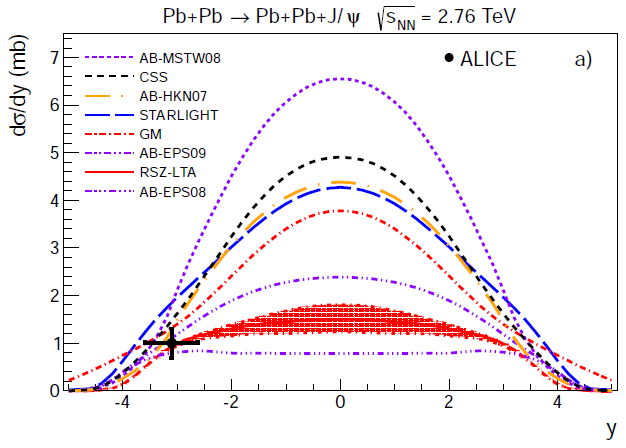
\includegraphics[width=0.5\textwidth,keepaspectratio]{aliceDsigDy.png}
    \end{center}
    \caption{ \label{fig:rapDepAll} AB is the pQCD method, RSZ-LTA is the LTA method, and STARlight
      is the VMD model.}
  \end{figure}
  In Fig.~\ref{fig:rapDepAll} at higher rapidities, in particular $|y|>3$, the 
    various models give similar values for $d\sigma/dy$. 
  At $y=0$ the models vary the most. 
  Fig.~\ref{fig:rapDepAll} shows that experiments that can measure $J/\psi$
    at $y=0$ have the best opportunity to distinguish between the models.
  The high sensitivity at $y=0$ creates an advantage for experiments that can 
    measure particles with small rapidity and low momentum.  
 
  The UPC photoproduction models each have different shapes to their rapidity 
    dependence. 
  The slope of $d\sigma/dy$ in Fig.~\ref{fig:rapDepAll} depends on the model. 
  Through the rapidity region $1<|y|<3$, each of the models has a progressively
    steeper slope. 
  The LTA method and the pQCD method utilizing the EPS08 gluon density model 
    are relatively flat where as the VMD and other gluon density models using
    the pQCD method have a noticeable slope.
  The differing slopes provide an additional experimental observable. 
  The shape of the rapidity distributions provide experimental sensitivity at 
    rapidities away from $y=0$ and creates an opportunity for experiments that 
    can not measure $J/\psi$ at $y=0$.

  The nuclear suppression factor, S, demonstrates the difference between how 
    the models represent the nucleus. 
  S, which is a ratio between the nuclear photoproduction cross section and the     
    free nucleon photoproduction cross seciton, is a measure of how the nuclear 
    gluon densities evolve in each of the models. 
  Fig.~\ref{fig:ltaAndPqcdNucSub} from Ref.\cite{lta2013.05} shows the nuclear 
    suppression, which is equivalent to $R_g$ in Eq.~\ref{eq:ltaOptTheWNucMo}, 
    for the LTA and pQCD method.
  \begin{figure}[h] 
    \begin{center}
      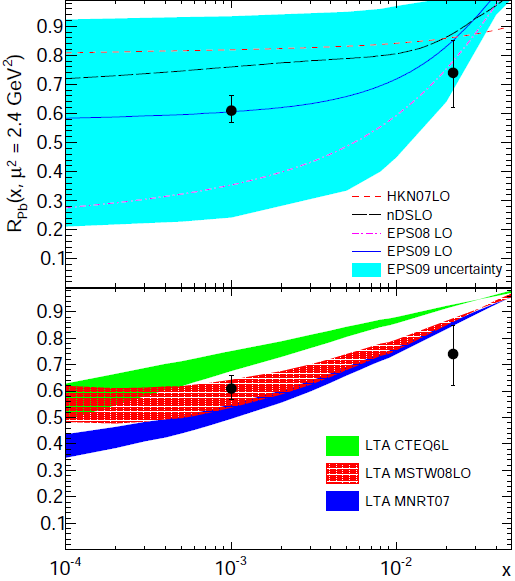
\includegraphics[width=0.5\textwidth,keepaspectratio]{ltaAndPqcdNucSub.png}
    \end{center}
    \caption{ \label{fig:ltaAndPqcdNucSub} Nuclear supression factor, $S$, in the pQCD and LTA methods.}
  \end{figure}
  \begin{figure}
    \begin{center}
      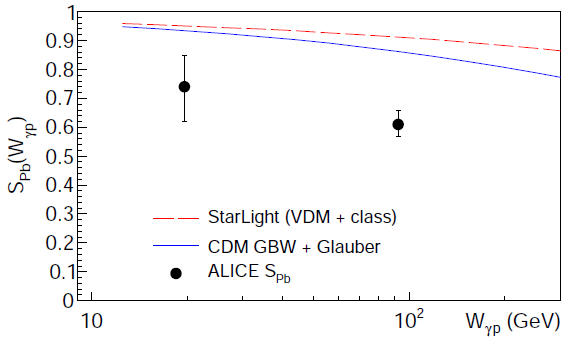
\includegraphics[width=0.5\textwidth,keepaspectratio]{ltaAndPqcdNucSubVMD.png}
    \end{center}
    \caption{ \label{fig:ltaAndPqcdNucSubVMD} Nuclear supression factor, $S$, in VMD method.}
  \end{figure}
  Fig.~\ref{fig:ltaAndPqcdNucSubVMD} shows the nuclear suppression for the VMD 
    method \cite{lta2013.05}. 
  Fig.~\ref{fig:ltaAndPqcdNucSubVMD} and Fig.~\ref{fig:ltaAndPqcdNucSub} show that 
    as the momentum of the probing photon goes up, increasing $W_{\gamma p}$, 
    and momentum of the probed gluon goes down, decreasing $x$, 
    the nuclear gluon density decreases relative to the free nucleon. 
  The nuclear suppression factor, S, allows for the different models' 
    representations of the gluon content of the nucleus to be directly compared
    to each other and to data. 
  S can be measured from data by assuming a Weizsi\"{a}cker-Williams photon flux and 
    provides insight into nuclear gluon densities. 

\chapter{The CMS Detector}	
CMS is housed at interaction point 5 of the LHC. 
The LHC is designed to pursue physics at the TeV scale. 
This is the scale where electroweak symmetry breaking is believed to occur
	\cite{CmsPTdrv2}.
While this means that the search for the standard model Higs is the central 
	driving design consideration, the wide range of possibilities for
	finding new physics signals requires a general purpose detector.
The expedient discovery of new physics through low cross section interactions 
	requires high luminosity.
This consideration leads inevitably to pile up, where multiple collisions 
	occurs at a single bunch crossing.
At peak luminosity the LHC is expected to produce on average 20 hard 
	proton-proton (pp) collisions per bunch crossing \cite{tCmsE}.
These particle physics considerations of high multiplicity due to pileup and the
	need for a general purpose detector make CMS serendipitously well suited
	for heavy ion physics.
\begin{figure}[h]
  \centering
    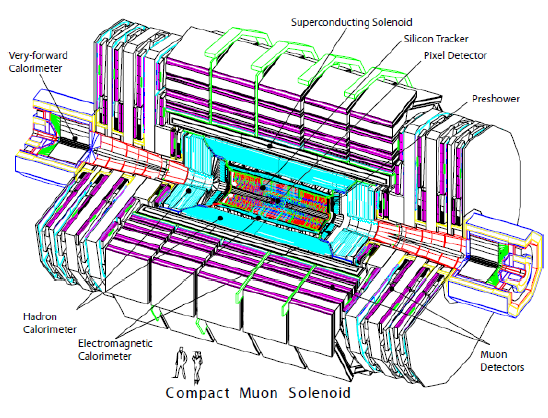
\includegraphics[width=.5\textwidth]{cms}
  \caption{The Compact Muon Solenoid from Reference~\cite{tCmsE}.}
  \label{cms}
\end{figure}

The general purpose design of CMS is dominated by the massive 4T 
	superconducting solenoid at its core.
The magnets is 13m long with a 6m diameter, and pushes the limits of power
	and compactness \cite{tCmsE}. 
These two conflicting limits are achieved through the novel design of 
	interweaving structural and conducting elements together in the coil of
	the solenoid.

Within the solenoid resides three different sub detectors.
The inner most is the world's largest silicon tracker \cite{tCmsE}.
The tracker is surrounded by a highly effective lead tungstate crystal 
	electromagnetic calorimeter (ECAL).
ECAL is encapsulated in a brass scintillating hadronic calorimeter (HCAL).
Outside the magnet, muon chambers are used to aid in the measurement and 
	triggering of muon events. 
Altogether CMS weighs 12,500 metric tons, has a diameter of 14.6m,
	and a length of 21.6m \cite{tCmsE}.

The Silicon Tracker is the innermost sub-detector of CMS, and has active
	elements as close as 4.4cm to the interaction point \cite{tCmsE}. 
The tracker has a length 5.8m, a diameter of 2.6m and
	covers a range in pseudorapidity of \(|\eta| <\) 2.5.
Pseudorapidity is defined as $\eta\equiv-\ln(\tan(\theta/2))$, where $\theta$ is 
	the polar angle, and $\phi$ is the azimuthal angle with respect to the 
	beam axis.
At the center of the tracker are three rings of silicon pixels around the beam 
	with two disks of silicon pixels to cap the rings.
The pixel portion of the silicon tracker is comprised of 66x10$^{6}$
	pixels.
The silicon pixels are surrounded by silicon strips.
The silicon strips are separated into 4 different sections: 
	the Tracker Inner Barrel, the Tracker Inner Disk, the Tracker Outer 
	Barrel, and the Tracker End Caps.
The silicon strip detectors as a whole are comprised of 9.3x10$^{6}$ silicon 
	strips.
The high number of pixels and strips allow for the ability to distinguish
	and collect enough distinct points to reconstruct the path of the 1000
	or so charge particles per bunch crossing expected at peak luminosity
	\cite{tCmsE}.  

The next detector beyond the tracker is ECAL.
ECAL is made of 61,200 lead tungstate (PbWO$_{4}$) crystals in the central
	barrel and 7,324 on each of the two endcaps \cite{tCmsE}.
The barrel (EB) covers a pseudorapidity range $|\eta| < 1.479$ and has an
	approximate $\eta-\phi$ segmentation of $0.0174\times0.0174$.
Lead tungstate is very dense, which is reflect in the high number of interaction
	lengths the short depth of one crystal provides.
The crystals of the barrel have a depth of 230 mm corresponding to 25.8 
	radiation lengths ($X_{0}$).
The radiation length is the mean distance a high energy particle travels before
	giving up one e-fold of kinetic energy through electromagnetic
	interactions.
For example, after one radiation length $E \rightarrow E/e$, where 
	$e = 2.71828183$. 
The endcaps (EE) cover the psuedorapitity region $1.479 < |\eta| < 3$.
In the endcap the crystals have an exposed area of 28.62 $\times$ 28.62 
	mm$^{2}$, and a depth of 220 mm corresponding to 24.7 $X_{0}$.
The energy resolution of the ECAL as measured by test beam data can be seen in
	Figure~\ref{ECALeRes}.
\begin{figure}[h]
  \centering
    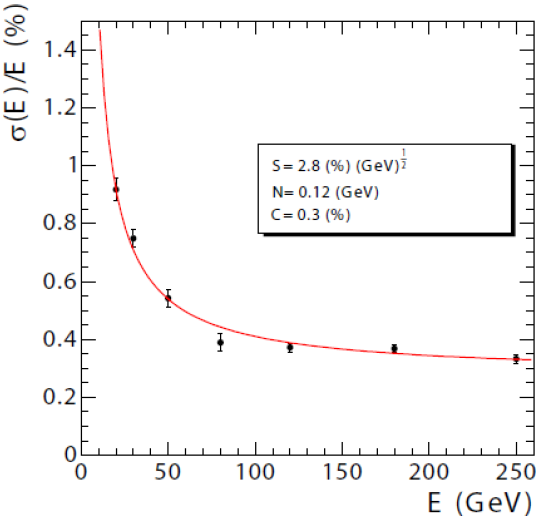
\includegraphics[width=0.5\textwidth]{ECALeRes}
  \caption{The energy resolution of ECAL as a function of energy from 
	Reference~\cite{tCmsE}.}
  \label{ECALeRes}
\end{figure}

The HCAL like the ECAL has both a barrel (HB) and endcaps (HE).
The pseudorapidity region $|\eta|<1.3$ is covered by HB \cite{tCmsE}. 
HB has an $\eta-\phi$ segmentation of $0.0897\times0.0897$, and is 25 times more
	sparsely granulated than EB.
HE covers the pseudorapidity region $1.3<|\eta|<3$.
HE, like EE and the tracker endcaps, is aligned perpendicular to the beam axis
	resulting in granularity that changes with $\eta$.
In the region $1.3 <|\eta|< 1.6$ HE has an $\eta-\phi$ segmentation of 
	$0.0897\times0.0897$.
The $\eta-\phi$ segmentation roughly doubles to $0.17\times0.17$ in the region
	$1.6 <|\eta|< 3$.
The energy resolution of the barrel and endcaps can be seen in  
	Figure~\ref{HCALeRes}.
The thickness of the hadronic calorimeter is best described in interaction
	lengths, the mean distance for a particle to give up an e-fold of energy
	through nuclear interactions. 
At $\eta = 0$ the barrel has a thickness 5.82 interaction lengths 
	($\lambda_{I}$), and increases as the path length through the material 
	increases to 10.6 $\lambda_{I}$ at $|\eta| = 1.3$.
\begin{figure}[h]
  \centering
    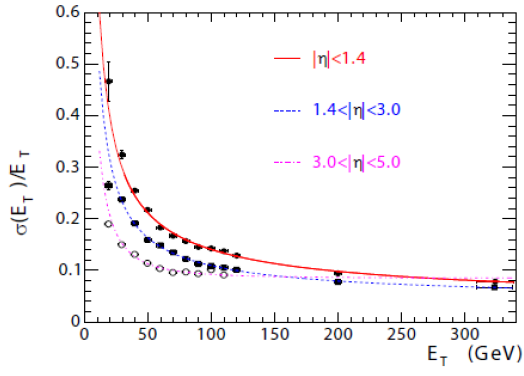
\includegraphics[width=0.5\textwidth]{HCALeRes}
  \caption{The $E_{T}$ resolution of HCAL as a function of $|\eta|$ and $E_{T}$
	from Reference~\cite{tCmsE}.}
  \label{HCALeRes}
\end{figure}

In addition to HB and HE, HCAL has two additional calorimeters.
Because the space between ECAL and the magnet is restricted to 1.18 m, an
	outer hadronic calorimeter section (HO) is placed beyond the magnet
	in the region $|\eta|<1.3$ \cite{tCmsE}.
The main function of HO is to collect energy from the highest energy hadrons
	before they reach the muon system.
HO is not used in this analysis, but does contribute to the material budget. 
To increase the total calorimetric coverage, HCAL also has a quartz fiber 
	calorimeter (HF) in the forward region, $3 < |\eta| < 5$.
For the majority of HF's 13 $\eta$ rings the $\eta-\phi$ segmentation is 
	$0.175\times0.175$.
In the lowest $|\eta|$ ring the segmentation is $0.111\times0.175$ in 
	$\eta-\phi$.
In the highest two $|\eta|$ rings the segmentation in $\phi$ is 0.349, with an
	$\eta$ segmentation of 0.175 in the outer and 0.300 in the innermost 
	ring. 
The longitudinal direction is effectively segmented by using short fibers and
	long fibers.
The measure energy deposited deeper than 22 cm is measured in both the short
	and long fibers, where as the long fibers are present throughout.
This allows electromagnetic showers to be distinguished from purely hadronic 
	showers \cite{tCmsE}.
The energy resolution for HF can be seen in Figure~\ref{HCALeRes}.  

Beyond HF there are two more detectors in the forward region.
CASTOR covers the range 5.2 $< \eta <$ 6.6 on the positive side of the beam. 
The Zero Degree Calorimeters (ZDC) sit between the beam pipes on either side of
	the interaction point covering the area around $\theta = 0$, $|\eta| > 
	8.3$.
In heavy ion collisions the ZDC has the ability to measure neutral particles 
	that do not participate in the collision \cite{tCmsE}.
CASTOR extends the total coverage of the CMS as whole giving more access to 
	low-x physics \cite{tCmsE}.

The ZDC has a total of 18 channels.
Half of these 18 channels are on either side of the interaction point.
The 9 channels on the side of CMS that correspond to positive $\eta$
  are denoted ZDC$^{+}$, where as the 9 channels on the negative side are
  denoted ZDC$^{-}$.
The 9 channels on each side are further sub-divided into an electro-magnetic  
  (EM) section and a hadronic (HAD) section.
The EM section is positioned in front of the HAD section with respect to the 
  interaction point and is segmented transverse to the beam direction.
The 5 EM sections are positioned in front to absorb the energy from 
  electro-magnetically induced showers, which develop over a shorter distance 
  than hadronically induced showers.
The transverse segmentation allows for a measurement of the transverse shower
  width and the size of the beam spot at the ZDC.
The HAD section is segmented in the direction of the beam and consists of 4
  channels.
The longitudinal segmentation allows for absorption of the full extended 
  hadronic shower and the ability to measure the longitudinal shower shape.

Each the 18 channels contains a tungsten target and quartz fibers.
The dense tungsten target is used to initiate the shower.
The quartz fibers shine Cerenkov light as the high momentum charged particles
  from the shower pass through it. 
the light from the quartz fibers is channeled to photo-multiplier tubes, one 
  for each ZDC channel. 
Through a cascade of photon induced electrical discharges, the photo-multiplier
  converts the Cerenkov light to an electrical pulse. 

This electrical pulse travels $\sim$ 200 m down a coaxial cable from the LHC
  tunnel to the counting house in the CMS service cavern. 
There the electrical pulse is digitized by the Charge Integrator and Encoder 
  (QIE).
The QIE integrates the current each 25 nano seconds.
The charge is than mapped logarithmically to the 128 bits. 
This bit is sent across a small fiber optic cable to the HTR firmware card.
Here each 25 ns signal is stored in a 250 ns buffer, and the timing is sync
  with the rest of the detector to insure the ZDC signal arrives at the central
  data acquisition system at the same time as the other sub detectors from the 
  same collision. 

The muon system resides just outside of the superconducting magnet.
It consists of three complementary systems: drift tube (DT) chambers in the
	barrel, cathode strip chambers (CSC) in the endcaps, and resistive 
	plate chambers (RPC) in both the barrel and endcap regions \cite{tCmsE}.
Ultimately the muon system is most useful for triggering on muons \cite{tCmsE}.

The heavy ion community is making use of the capabilities of CMS in a myriad of
	ways.
The muon trigger has been used in the search for suppression of quarkonium 
	states. 
This is an important probe of the correlation length within the hot dense state
	known as the quark gluon plasma (QGP).
The tracker has been utilized for to study charged particle multiplicities, and
	and elliptical flow, two probes of the thermal expansion of the QGP.
HCAL has aided in measuring jet suppression, which probes the strength with 
	which the QGP interacts with strong interacting objects.
Through its general purpose design and its ability to handle the high
	multiplicities produce by the LHC, CMS proves to be an excellent 
	detector for investigating strongly interacting mater through heavy ion
	collisions. 
%  \section{CMS general}
%  \section{Muons}
%  \section{HCal}
%  \section{ZDC}
  \section{Trigger}
    The CMS trigger is two teired. 
    The L1 trigger is the lower level hardward based system. 
    The High Level Trigger (HLT) is software base and runs on a computer farm
      at point 5 where CMS is housed.

    The purpose of the L1 trigger is to make quick decisions about which events
      will be kept temporarily for for further processing.
    The L1 trigger is used to identify events where the tracker should be read
      out.
    Only the calorimeters and the muon system are used in the L1 trigger.
    Each of the sub-detectors has it's triggering hardware.
    The output from the sub-detectors is synchronized to ensure that the signal
      from each of the sub-detectors comes from the same collision. 
    The global trigger hardware then makes the final decision to initiate the 
      HLT and to read out the tracker. 

    If an event passes the L1 trigger, the data from all the sub-detectors in
      including the Tracker are sent to the HLT computing farm. 
    At this level the raw data from all the sub-detectors is unpacked and 
      combined.
    The information from the calorimeters, muon system, and tracker can all 
      be used to reconstruct basic physic objects in the HLT farm. 
    For example, tracks can be combined with either ECAL energy clusters to 
      form electron candidates, tracks can be combined with hits in the muon
      system to create muon candidates.
    At the HLT the whole detector is used together to select events.
    The raw data from the events that survive the HLT are recorded permanently,
      those that do not are lost forever. 

    The HLT farm must always be ready to accept events from the L1 trigger.
    For this reason, the amount of computing time each HLT trigger path uses
      must be balanced.
    For more rare L1 triggers, which will occur at a lower rate, more 
      complex reconstruction software can be used.
    Conversely, simpler, faster, methods must be used for more common high
      rate triggers. 
    Because of this time constraint in the HLT farm, the reconstruction 
      algorithms used for triggering tended to differ from the final 
      reconstruction algorithms.
    In the HLT these algorithms are optimized for quickness, whereas the final 
      reconstruction is optimized for precision and accuracy.
    By having the ability to spend different amounts of computing time on 
      different L1 triggered events, the complexity of the event selection 
      offered by the HLT is heightened. 

    The two tiered triggering system creates very low dead times while 
      maintaining purity and selectivity.
    During data taking the L1 trigger is continuously monitoring, and the HLT
      allows for sophisticated event selection.
    The wide gamete of physics topics that are pursued by the CMS collaboration
      are a testament to the effectiveness and versatility of the CMS two 
      tiered triggering system. 

\chapter{Analysis}
  In this chapter the various parts of the analysis are explained. 
  In Section~\ref{sec:mcSim}, the simulations used to estimate the detector's 
    ability to measure UPC processes are discussed. 
  Section~\ref{sec:TrigDev} explains the considerations that went into the 
    triggers that were developed for this measurement.
  The event selection for the various data sets is detailed in 
    Section~\ref{sec:DataSetEvSel}.
  Extraction of the number of events from each of the three physics processes 
    discussed in this thesis, coherent, incoherent, and photon-photon process
    is discussed is Section~\ref{sec:sigEx}.
  The determination of the detectors efficiency for measuring UPC events is 
    explained in Section~\ref{sec:effDet}.
  Finally, Section~\ref{sec:sysCheck} lays out the systematic uncertainties 
    estimates for the measurements.

  \section{\label{sec:mcSim} MC simulation}
    Every physical measurement is the product of the underlying physics 
      folded with the response of the detector used to do the measurement. 
    In order to understand the underlying physical process, the detector's 
      effect on the measurement must be understood and accounted for. 
    As instruments become more and more complicated, the interplay between all
      of the many parts of the detector makes an analytic approach to the 
      problem untenable.
    For this reason, the numerical technique of Monte Carlo (MC) simulation is
      the most useful approach.

    MC simulations use random number generation to solve the problem 
      numerically by brute force. 
    First, particles are generated according to theoretical distributions.
    These particles are then propagated through a simulation of the detector.
    As the particles pass through the detector, random numbers are again used
      to determine how these particles interact with the materials of the 
      detector based on the known properties of the material. 
    In this way, the theoretical distributions are convolved with a realistic 
      model of the detector's response. 
    A more detailed picture of how the detector shapes the underlaying 
      distributions with each successive event. 
    The set of events that are produced resemble as closely as possible the 
      results that would be seen were the physical process to be measured 
      by the detector.
    
    In this thesis, two main classes of MC simulation samples were used, 
      STARlight and a particle gun.
    The STARlight samples corresponds to the theoretical calculations 
      described in Section~\ref{sec:vdmTheory}, while the particle gun produces
      particles with a user defined momentum distribution. 
    For STARlight three different physical process are simulated;
      coherent \JPsi{} production, where the photon couples to the nucleus as
      a whole, incoherent \JPsi{} production, where the photon couples to a
      nucleon within the nucleus, and photon-photon interactions, where the 
      photons from the two nuclei interact with each other to produce a pair 
      of oppositely charge muons directly.
    All three STARlight samples contain a $\mu^{+}$ and $\mu^{-}$ in the final 
      state.
    The second class uses PYTHIA6 to decay \JPsi{}s produced with a user 
      defined \pt{} and rapidity distribution into muon pairs.

    Because STARlight is not integrated into the standard CMS software 
      framework (CMSSW), a simulation software chain with 5 steps was developed.
    First, STARlight is run in the specified mode, and a single file is 
      created for each physics process. 
    In step 2 the STARlight output file is converted to the Les Houches (LHE) 
      format \cite{lheFormat}, and the momentum of the parent \JPsi{} or the 
      initial photon-photon pair is added to the record of each event.
    The event record produced by STARlight only contains the final state 
      particles.

    To process the events in parallel, the STARlight files are subdivided 
      into in step 2, creating several LHE files from a single STARlight file.
    The LHE files are used as input to CMSSW.
    Steps 3 to 5 take place within CMSSW. 
    In step three the generated particles are propagated through the GEANT4 
      \cite{geant} detector simulation.
    This accounts for all the interactions with the detector and produces as 
      output a format identical to the raw data that is recorded during data
      taking.
    Steps 4 and 5 are processed using the same software as in data taking.
    In step 4 the reconstruction software used during data taking is run on 
      the output of the detector simulation
    The output of the reconstruction is reduced to the information that is 
      needed for the final analysis in the final step.

    The particle gun samples were created entirely within CMSSW.
    \JPsi{} mesons were created according to user defined \pt{} and rapidity
      distributions. 
    PYTHIA6 \cite{pythia} decays the \JPsi{}s to $\mu^{+}$ and $\mu^{-}$.
    As with the STARlight samples, these muons are propagated through the GEANT4
      simulation of the detector, and the raw data is produced.
    The remaining steps of running the reconstruction code and reducing the 
      data to the final data needed for the analysis are identical to the 
      STARlight production.

    The various MC samples differ primarily in the 
      \pt{} distribution and the polarization of the \JPsi{}s produced. 
      The polarization of the \JPsi{} effects the angle at which the muon daughters
      are emitted relative to the direction in which the \JPsi{} is traveling 
      \cite{oniaPol}. 
    In Fig.~\ref{fig:starlightRapPtDist} the \pt{} of \JPsi{}s from the 
      coherent and photon-photon samples are peaked steeply a low \pt{}, and 
      neither sample extends much beyond 0.15 GeV in \pt{}.
    The incoherent sample is peaked near 0.5 GeV and extends beyond 1 GeV.
    The two particle gun samples resemble the incoherent and coherent samples.
    The first sample has a Gaussian \pt{} distribution extending to 
      approximately 0.15 GeV, whereas the second is flat in \pt{} up to
      2 GeV.
    The particle gun samples are unpolarized, whereas the STARlight samples 
      have transverse polarization. 
    Therefore, the particle gun samples there is no preferred direction for the 
      emission of the daughter muons.
    In the STARlight samples however the daughters tend to be emitted in line
      with the direction of the \JPsi{}'s momentum.
    This is particularly pronounced for the photon-photon process.

    \begin{figure}[!Hhbt]
      \centering
      $ \begin{array}{cc}
        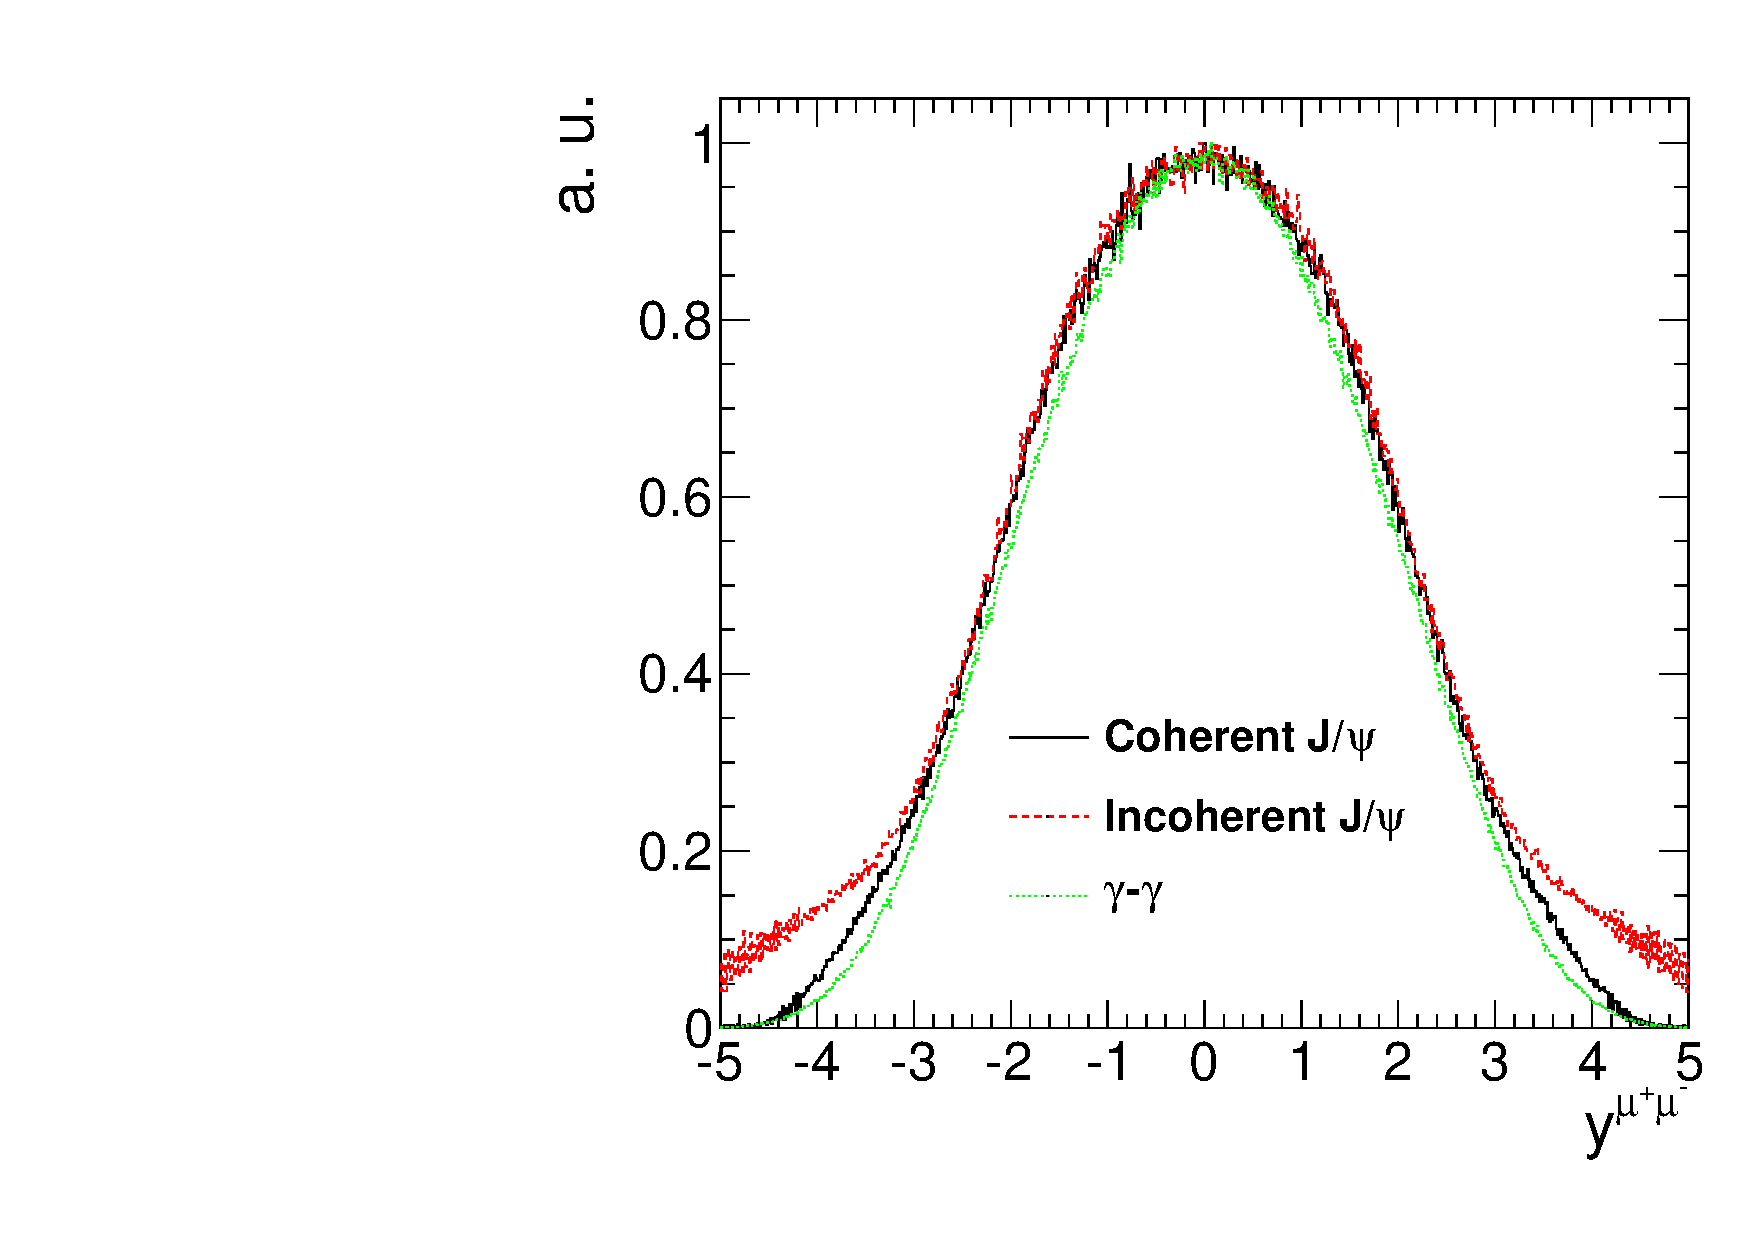
\includegraphics[width=0.45\textwidth]{genRapDis} &
        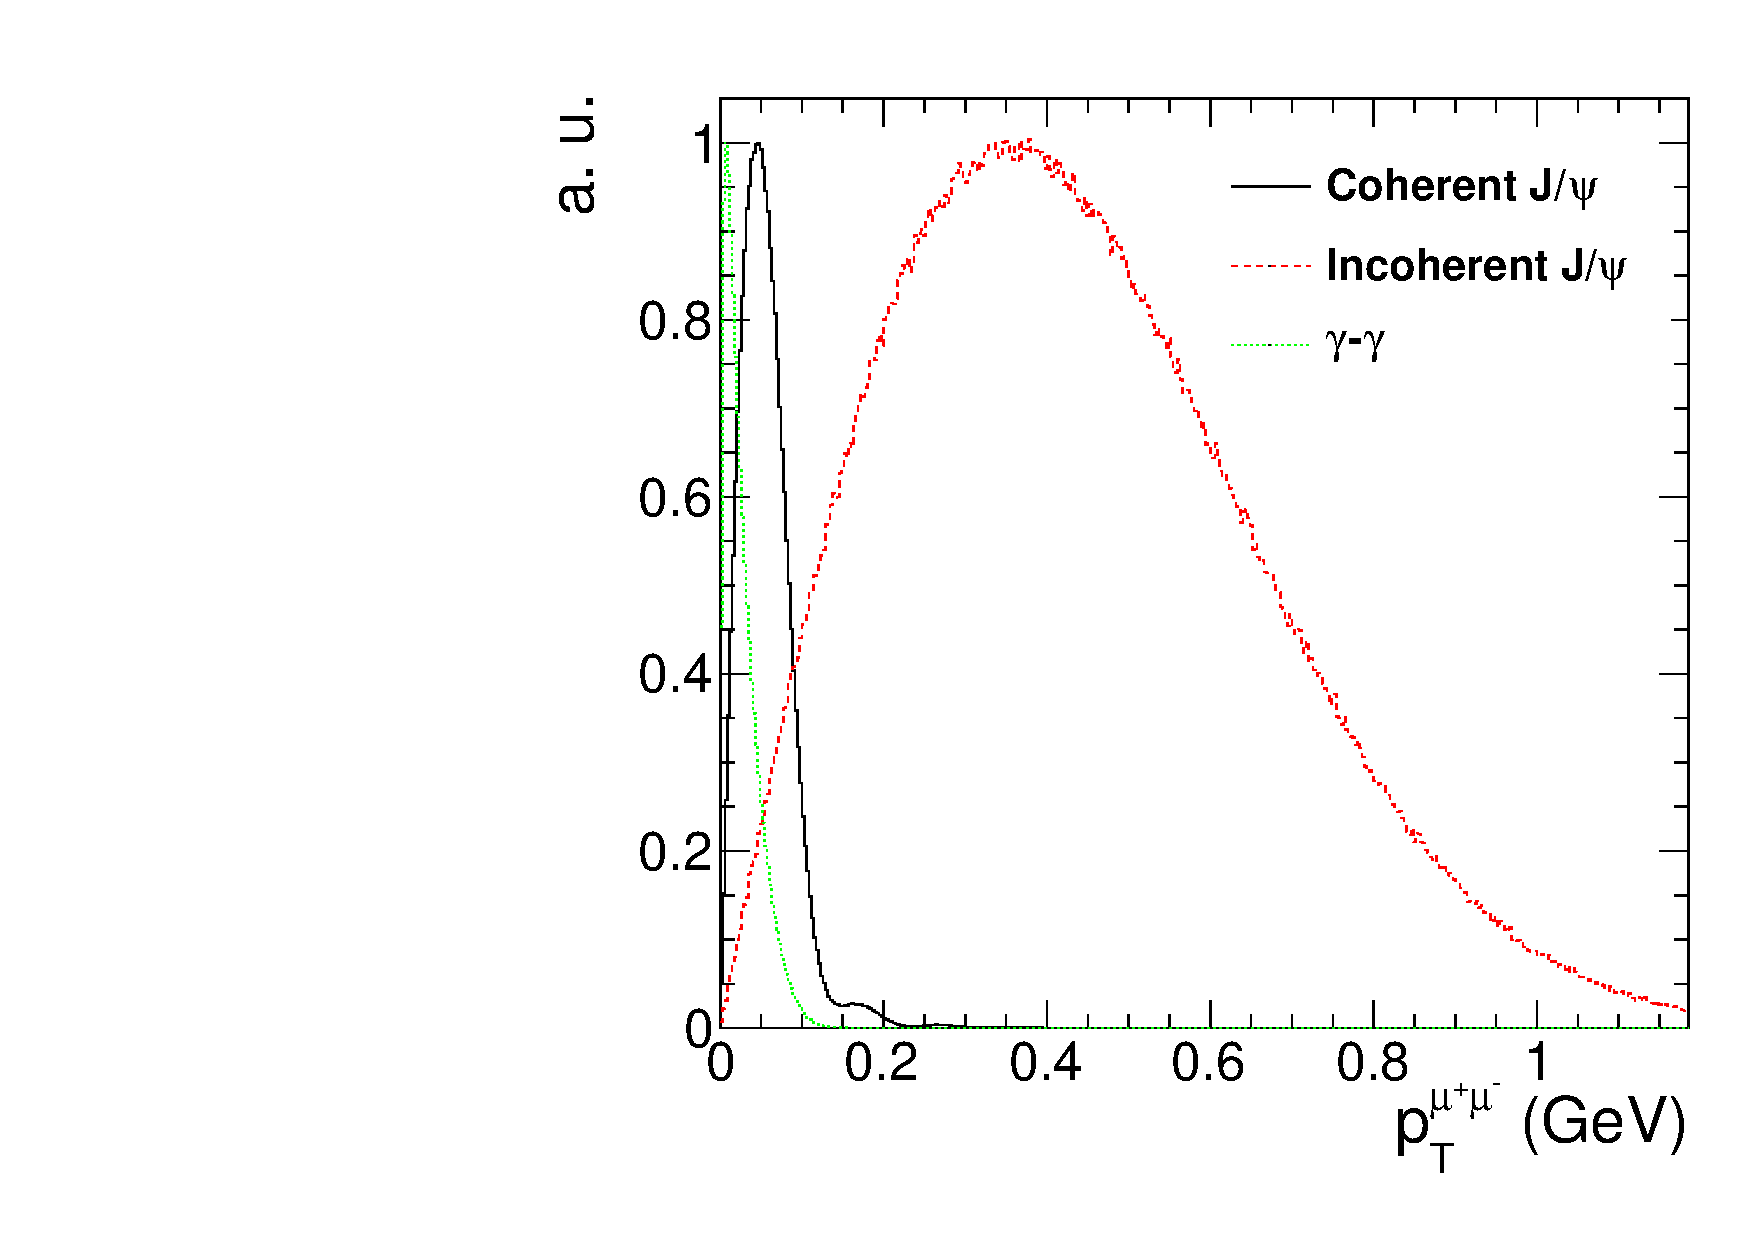
\includegraphics[width=0.45\textwidth]{genPtDis}
      \end{array} $
      \caption{Generator level rapidity (left) and \pt{} (right) 
          distributions for the coherent (black), incoherent (red), 
          and photon-photon process (green).}
      \label{fig:starlightRapPtDist}
    \end{figure}
    
    \begin{figure}[!Hhbt]
      \centering
      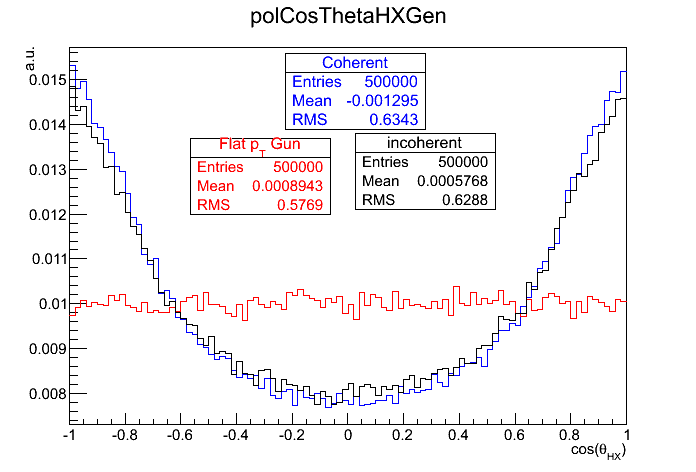
\includegraphics[width=.6\textwidth]{polCosThetaHXGen}
      \caption{ The \JPsi{} polarization of the particle gun (red),
        coherent (blue), and incoherent samples are plotted as the
        cosine of the helicity angle.} 
      \label{fig:genHXAngle}
    \end{figure}
%%%%%Fix this paragraph%%%%%%
    The momentum of the final state muons is the main drivers of whether the 
      candidate can be measured.
    If neither muon daughter of the \JPsi{} possess enough momentum to reach 
      the muon chambers and fire the trigger, the event will not be recorded.
    The polarization and the \pt{} distribution of dimuons from the generator
      determine the momentum of the daughters. 
    The polarization effects how the momentum is shared between the daughters.
    In the rest frame of the parent particle from which the daughters decay,
      equal momentum is given to each daughter. 
    However in the lab frame of the detector, the muon daughters which are 
      emitted from transversely polarized \JPsi{} will tend to be emitted in
      the direction of \JPsi{} and will have unequal momentum in the lab 
      frame.
    The daughter traveling in the direction of the \JPsi{} will have increased
      momentum, whereas the daughter traveling opposite to the \JPsi{} 
      direction will have decreased momentum. 
    The momentum of the lower momentum muon daughters is the main restriction
      on whether or not the \JPsi{} can be reconstructed in CMS. 
%%%%%Fix this paragraph%%%%%%
    
  \section{\label{sec:TrigDev} Trigger development} 
    The increase in collision rate of the LHC PbPb beams from 2010 to 2011 was
      nearly a factor of 15. 
    To accommodate this increase in rate, the 2011 trigger scheme needed to be 
      more selective than in 2010 where CMS could take any event which 
      appeared to have a collision.
    The available bandwidth was allocated equally amongst the various heavy ion
      analysis groups to pursue as wide a physics program as possible.
    From this consideration, bandwidth limits were placed on the trigger rates
      for each analysis group's trigger package. 
    To ensure that UPC physics could be explored all while respecting the
      goals of the CMS Heavy Ions group as a whole, a collection of UPC triggers
      were commissioned. 
  
    The UPC triggers were estimated by combining existing triggers from
      the 2010 run. 
    By calculating the ratio between the UPC trigger rates and the minimum bias
      trigger rate, the UPC trigger rates were scaled up to the anticipated 2011 
      interaction rates using the 2010 data.
    The trigger package for 2011 contained ZDC based efficiency monitoring 
      triggers, muon and electron based triggers for measuring \JPsi{}, and 
      backup triggers in case there was a problem with the original muon and 
      electron triggers.

    \subsection{\label{sec:l1Trigger} L1 trigger}
      The goal of the UPC L1 triggers was to record enough data to measure 
        UPC \JPsi production via the dimuons and dielectrons channels.
      To achieve this, the loosest muon and electron triggers where paired with
        a trigger on energy in the ZDC and a veto on energy in the BSCs.
      Additional triggers that vetoed on energy in HF were commissioned in case
        radiation damage during the run reduced the sensitivity of the BSCs.
      These triggers are summarized in Table~\ref{tab:l1Triggers2011}.
      The 5 and 2 for the ECAL triggers in Table~\ref{tab:l1Triggers2011}
        indicate a 5 and 2 GeV threshold on $E_{T}$ measured in the ECAL.
      The Open in the muon trigger indicates that the trigger only 
        requires a muon candidate in one of the three muon sub-systems and that
        there is not momentum threshold.

      \begin{table}[h]
        \centering
        \begin{tabular}{|l|l|l|l|l|}
          \hline L1 trigger & Rate (Hz) & Prescale & Id & Type \\ \hline \hline
          MuonOpen and (ZDC$^{+}$~or~ZDC$^{-}$) and BSC veto & 2.1 & 1 & 1 & \multirow{3}{*}{Physics} \\  \hhline{----~}
          ECAL2 and (ZDC$^{+}$~or~ZDC$^{-}$) and BSC veto & 1.8 & 2 & 2 & \\  \hhline{----~}
          ECAL5 and (ZDC$^{+}$~or~ZDC$^{-}$) and BSC veto & 0.3 & 1 & 3 & \\  \hline
          (ZDC$^{+}$~or~ZDC$^{-}$) & 35 & 1500 & 4 & Monitor \\  \hline
          MuonOpen and (ZDC$^{+}$~or~ZDC$^{-}$) and HF veto & 0 & off & 5 & \multirow{3}{*}{Backup} \\ \hhline{----~}
          ECAL2 and (ZDC$^{+}$~or~ZDC$^{-}$) and HF veto & 0 & off & 6 & \\  \hhline{----~}
          ECAL5 and (ZDC$^{+}$~or~ZDC$^{-}$) and HF veto & 0 & off & 7 & \\  \hline
        \end{tabular}
        \caption{List of 2011 L1 seeds.}
        \label{tab:l1Triggers2011}
      \end{table}
      The cumulative L1 trigger rate for all the UPC L1 trigger seeds was
        required to be 200 Hz.
      This requirement stemmed from the need to keep the tracker read-out rate
        low. 
      The trackers baseline voltage can fluctuate due to the high tracker hit 
        multiplicities in PbPb collisions.
      In order to monitor the zero suppression of the tracker, the zero 
        suppression algorithm was executed using the HLT computing farm 
	      rather than in the tracker firmware.

      In order to record the efficiency monitoring data, the ZDC triggers had 
        to be prescaled to a lower rate. 
      The scaling down of the monitoring trigger was setup to insure overlap
        with the signal triggers.
      The prescales for the triggers were set to balance the competing objectives 
        of rate reduction and increasing the overlap between the monitoring and
        signal triggers.

    \subsection{HLT trigger}
      As opposed to the L1 trigger, which has access only to information from
        calorimeters and muon chambers, the HLT has access to all the 
        sub-detectors including the tracker. 
      Reconstruction of a track in the pixel detector is used by the UPC 
        trigger paths.
      The use of the pixel detector only, as opposed to using the whole tracker 
        including the silicon strip detector, allows for quick track 
        reconstruction saving computing cycles.
      The requirement of at least one reconstructed pixel track for the HLT 
        triggers was designed to reject backgrounds where no particles are 
        reconstructed by the tracker.
      For the muon trigger in Table~\ref{tab:hltTrigger2011} the rate was 
        reduced by nearly a factor or 4 compared to its L1 seed rate in 
        Table~\ref{tab:l1Triggers2011}.
      This is due to the additional pixel track requirement. 
      \begin{table}[h]
        \centering
        \begin{tabular}{|l|l|l|l|l|l|}
          \hline HLT trigger  & Rate (Hz) & L1 prescale & HLT prescale & L1 seed & Type \\ \hline \hline
          L1UPCMuon and Pixel Track & 0.52 & 1 & 1 & 1 & \multirow{3}{*}{Physics} \\ \hhline{-----~} 
          L1UPCECAL2 and Pixel Track & 1.65 & 2 & 1 & 2 & \\ \hhline{-----~}
          L1UPCECAL5 and Pixel Track & 0.26 & 1 & 1 & 3 & \\ \hline
          L1ZDCOr & 3.6 & 1500 & 11 & 4 & \multirow{2}{*}{Monitor}  \\ \hhline{-----~}
          L1ZDCOr and Pixel Track & 2.8 & 1500 & 1 & 4 & \\ \hline
          L1UPCMuonHFVeto and Pixel Track & 0 & off & off & 5 & \multirow{3}{*}{Backup}   \\ \hhline{-----~}
          L1UPCECAL2HFVeto and Pixel Track & 0 & off & off & 6 & \\ \hhline{-----~}
          L1UPCECAL5HFVeto and Pixel Track & 0 & off & off & 7 & \\ \hline 
        \end{tabular}
        \caption{List of 2011 HLT trigger.}
        \label{tab:hltTriggers2011}
      \end{table}

      The total HLT output for the UPC trigger package was 20 Hz. 
      The limiting factor for the HLT rate was the amount of disk space 
        available to store the data. 
      To meet the bandwidth requirements and collect a significant sample
        of data for estimating efficiencies, the prescales were balanced with 
        the goal of achieving at least 5\% statistical precision on the 
        efficiency estimates. 
      As an example of the balancing of the prescales, the  ZDC trigger that 
        was passed through from the L1 was given a additional prescale factor 
        of 11 on the HLT.
      The ZDC path that also required a pixel track on the HLT, which used 
        the same L1 seed, was only prescaled at the L1.
      The prescale of 11 was set to ensure that at least 1000 of the pixel track 
        ZDC triggers overlapped with the ZDC L1 only triggers so that efficiency
        of the pixel track requirement in the trigger could be estimated from 
        the tracks lost. 

  \section{\label{sec:DataSetEvSel} Event selection}
    In order to investigate novel physics processes like UPC \JPsi{} 
     production, the LHC has delivered unprecedented amounts of data.
    The data for this analysis was recorded during the 2011 LHC PbPb run. 
    During this period, 150 $\mu$$b^{-1}$ where recorded by the CMS detector,
      corresponding to over a billion PbPb collisions. 
    Of this, 143 $\mu$$b^{-1}$ were used in this analysis.
  
    \subsection{Data sets}
      Three specially selected samples were used for the present analysis, 
        Physics, Monitoring, and Zero bias, see Table~\ref{tab:sampleLumiNevt}.
      By recording this hierarchy of samples, interesting events are selected 
        with a much higher purity in the physics sample, while the zero bias and 
       ZDC triggered samples allow for the investigation of the selection 
        criteria. 
      These samples were recorded using subsets of the HLT triggers found in 
        Table~\ref{tab:hltTriggers2011} of Section~\ref{sec:TrigDev}.
      The \JPsi{} events discussed in this thesis were obtained analyzing the 
        sample labeled in Table~\ref{tab:sampleLumiNevt} as physics.
      A ZDC triggered monitoring sample was recorded for the sake of estimating
        efficiencies.
      Lastly, a zero bias sample was recored for investigating the ZDC and the 
        noise distributions of HF.
  
      To record the physics sample containing the \JPsi{} signal, a muon trigger
        was paired with a veto on energy in the BSC and a requirement that there 
        be energy in at least one of the two ZDCs. 
      This trigger utilizes the unlikely chance of having overlapping noise in
        in the ZDC and muon detector.
      Because of the characteristically low momentum of UPC \JPsi{} as compared
        to \JPsi{} created by any other physics process, the loosest muon 
        trigger was used.
      By pairing the muon trigger with the ZDC on the L1, the noise contribution
        was reduced from the noise contribution from either of the two 
        sub-detectors to the noise coincidence between the two sub-detectors. 
      Contributions from hadronic interactions are reduced by the veto on the 
        BSC.
      In this way, the balance between reducing the rate and maximizing the 
        efficiency was struck, allowing for the data to be recorded without 
        producing high rates resulting in dead time for the detector.  
      
      In order to investigate the muon trigger and the other parts of the event 
        selection, a minimum bias sample was recorded using the ZDC. 
      For ZDC triggered sample, any event which had energy consistent with at 
        least one neutron in either of the two sides of the ZDC was recorded.
      This process is much more common than the UPC \JPsi{} production.
      For this reason, the rates of this trigger are much higher than the physics
        trigger, and only a small sub set of these events are recorded.
      From this trigger the pixel track portion of the HLT trigger efficiency 
        was estimated. 
  
      In addition to the minimum bias and physics sample, a zero bias sample was 
        recorded to examine the ZDC trigger and the HF noise distributions. 
      The zero bias trigger fired every time both beams passed through CMS. 
      Only 4 events out of every million triggered were recorded for this sample. 
      This sample allowed for an unbiased measurement of the ZDC trigger 
      efficiency as discussed in Section~\ref{sec:effDet}. 
      Because the zero bias trigger does not require any activity in any of the
        CMS sub detectors, the sample contains very few hadronic collisions. 
      This allowed for a measurement of the electronic noise distributions in
      the HF, which will be discussed below.
  
      The integrated luminosity for each of the three samples is calculated
      by recording activity in HF \cite{cmsLumi}. 
      The cross section for HF activity is measured from a van der Meer scan, 
        and the cross section was found to be \textcolor{red}{X}.
      In this way the amount of integrated luminosity for any running period is
        related to the activity in HF. 
      \begin{table}
  	    \centering
  	    \begin{tabular}{|l|l|l|}
  	      \hline Sample & Events & $\mathcal{L}_{int}$ \\ \hline \hline
          Physics & 346K & 143.3 $\mu$$b^{-1}$ \\ \hline
          Monitor & 1.1M & 31.6 $mb^{-1}$ \\ \hline
          Zero Bias & 8.8M & 580 $b^{-1}$ \\ \hline 
  	    \end{tabular}
  	    \caption{Integrated luminosities and number of events for the three
  	      samples used in this analysis.}
  	    \label{tab:sampleLumiNevt}
      \end{table}
  
    \subsection{Event selection cuts}
      The analysis described in this thesis focuses on UPC \JPsi{}s decaying to 
        muons. 
      The trigger used for this analysis recored 346841 events.
      A set of off-line cuts were applied to increase the relative contribution 
        of UPC events to background processes. 
      Two sets of event selection cuts were applied to reject background events. 
      The first set rejects background from the beam.
      The second rejects events where hadronic collisions have occurred.
      The cuts in Table~\ref{tab:evSelCutNumbers} were applied. 
 
      \begin{table}
        \centering
        \begin{tabular}{|c|c|c|} \hline 
          Cut type & Cut & Events \\ \hline
          -- & all triggered & 346841 \\ \hline
          \multirow{3}{*}{beam background rejection} & good vertex requirement & 340997 \\ \hhline{~--}
          & beam halo muon rejection & 302777 \\ \hhline{~--}
          & cluster shape compatibility requirement & 233590 \\ \hline
          \multirow{3}{*}{hadronic interaction rejection} & single-sided neutron requirement & 149992 \\ \hhline{~--}
          & two track requirement & 32732 \\ \hhline{~--}
          & HF signal rejection & 5392 \\ \hline
          fake muon rejection & muon quality requirement & 2047 \\ \hline
          \multirow{2}{*}{kinematic cut} & \JPsi{} mass requirement & 696 \\ \hhline{~--}
          & muon detectability cuts & 567 \\ \hline
        \end{tabular}
        \caption{Effects of event selection cuts.}
        \label{tab:evSelCutNumbers}
      \end{table}
      
      To reject beam induced background the following cuts were applied:
      \begin{itemize}
        \item The reconstructed vertex must be within \textcolor{red}{X} cm in 
          the transverse direction and \textcolor{red}{X} cm in the 
          longitudinal direction. This cut insures that reconstructed particles 
          come from interactions between the two beams rather than event where 
          one of the two beams interact with gas particles near the interaction 
          point. 
  	    \item Beam halo muons were rejected using the timing of the muon hits.
              The beam halo cut rejects events where muons surrounding the beam 
              stream through the detector. 
  	    \item Pixel cluster shape should be compatible with the vertex. 
          This cut requires that energy deposits in the silicon tracker point 
            back to the reconstructed  primary vertex. 
      \end{itemize}
      These beam background cuts do not reject any UPC \JPsi{} candidates. 
  
      The second set of background rejection cuts were designed to 
        reduce contamination from hadronic interactions. 
      \begin{itemize}
  	    \item No more than 2 reconstructed tracks in the event.
          The track requirement rejects events that produce many charged 
          particles.
  	    \item Maximum reconstructed hit energy in HF was required to be below 
            the threshold for electronic noise. 
          Nearly all hadronic interactions (about 98\%) produce particles in 
            the range $3<|\eta|<5$ covered by the HF detector.
          By requiring that the energy deposits in HF resemble noise, nearly all
            elastic hadronic collisions are expected to be rejected.
  	    \item Energy in the ZDCs consistent with neutrons on only one side 
            of the interaction point.
          In hadronic interactions both nuclei break-up. 
          By requiring that ZDC only reconstruct neutrons on one side of the 
            interaction point, hadronic interactions that produce neutrons on 
            both sides were rejected.
      \end{itemize}
      Each of these cuts were designed to reject topologies produced by 
        hadronic interactions.
      The effect of these cuts can be seen in Table~\ref{tab:evSelCutNumbers} 
        and are denoted hadronic interaction rejection. 

      To establish the HF noise thresholds, the noise distributions were 
        measured in zero bias events. 
      Only presences of both beams was required for these events to be recorded. 
      An offline selection of events with no reconstructed tracks was used
        to ensure that no collision had taken place. 
      The HF noise threshold was defined as the cut that keeps 99\% of the 
        zero bias events.
      The noise distribution from this zero bias sample is compared to the 
        physics sample and MC in Fig.~\ref{fig:hfNoiseDist}.

      \begin{figure}[!Hhbt]
        \centering
        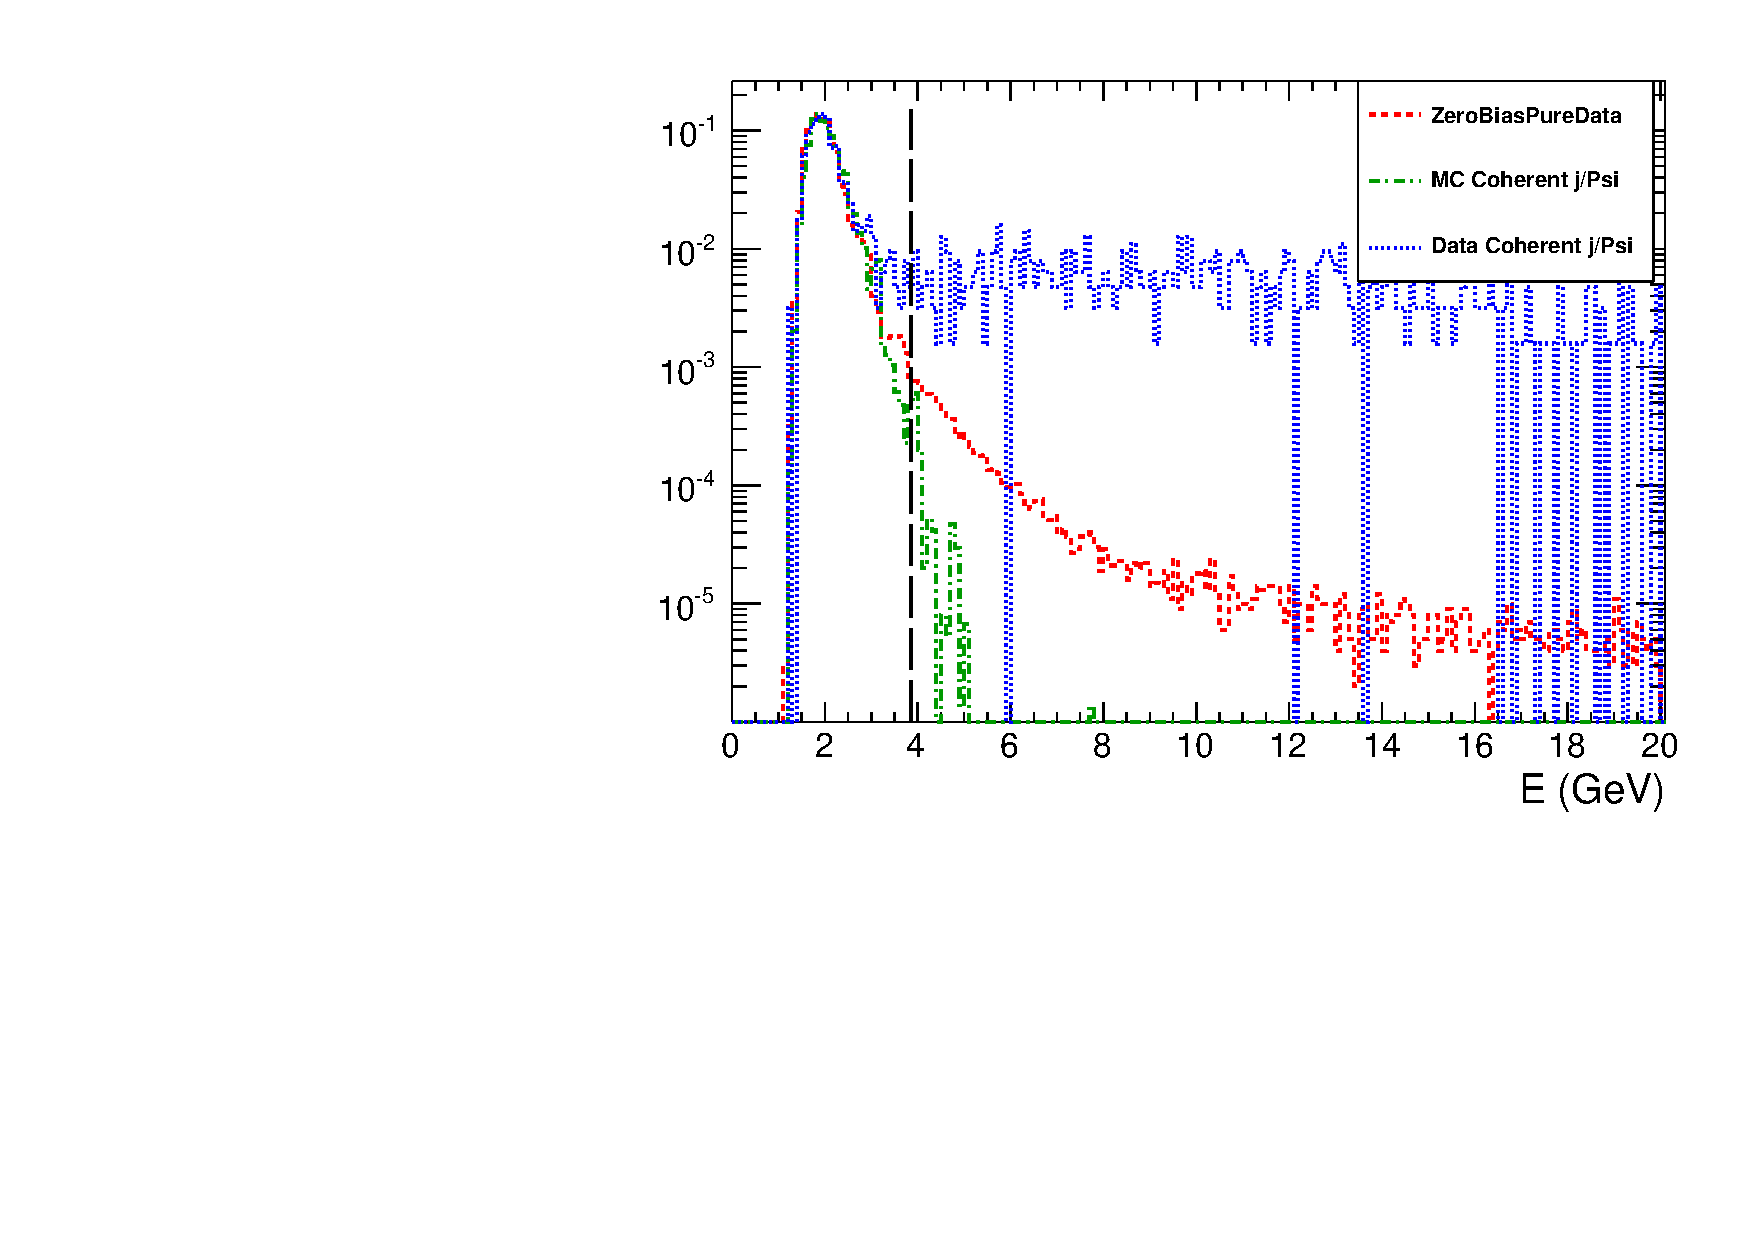
\includegraphics[width=.6\textwidth]{hfNoiseComp}
        \caption{Comparison of HF noise distributions in zero bias data, 
          physics triggered data, and MC.}
        \label{fig:hfNoiseDist}
      \end{figure}

      The following standard muon quality cuts are applied:
      \begin{itemize}
        \item Tracker track matched with at least one muon segment 
          (in any station) in both X and Y coordinates (< 3 $\sigma$).
        \item Cut on number of tracker layers with hits $>$ 5.
        \item Number of pixel layers $>$ 0.
        \item The $\chi^{2}$ per degrees of freedom of the track fit $<$ 3. 
        \item Loose transverse and longitudinal impact parameter cuts, with in 3 
          cm in the transverse direction and withing 30 cm in the longitudinal 
          direction with respect to the primary vertex.
      \end{itemize}
      These cuts are applied to reduce the number of fake muons and have been 
        validated for standard muon analyses.

  \section{\label{sec:breakUpDet} Break up determination}
    As described in Section~\ref{sec:ltaTheory}, UPC \JPsi{} photoproduction 
      can be accompanied by the emission of neutrons from either of the two 
      colliding nuclei.
    The various neutron emission scenarios, or break-up modes, can 
      be distinguished by the ZDC.
    By separating events where the ZDC signal is consistent with 1 neutron 
      versus several neutrons, the different break-up modes can be separated
      and compared to theory. 
    For this reason, reconstruction of the ZDC signal plays an important role 
      in this thesis. 
    In order to maximize the ability to explore the one neutron peak, which 
      sits at the bottom of the ZDCs dynamic range, a new ZDC reconstruction 
      method was devised. 
    This new reconstruction method was then used to establish a one neutron and
      many neutron threshold.
    In this section the ZDC signal reconstruction is described and how the 
      neutron thresholds on this signal were set.
    
    \subsection{ZDC signal reconstruction}
      The ZDC signal is built up from the pulse shapes for each of the 
        18 individual ZDC channels. 
      The pulse shape is recorded in 250 ns second chunks and is divided into
        10 time slices of 25 ns (See Fig~\ref{fig:zdcPulseShape}).
      Counting from 0, the 4th time slice is synced with the timing of the rest
        of the detector and corresponds to when the products of the recorded 
        collision reached the ZDC.
      For this reason the channel signal is taken from the 4th time slice.
      \begin{figure}[h]
        \centering
        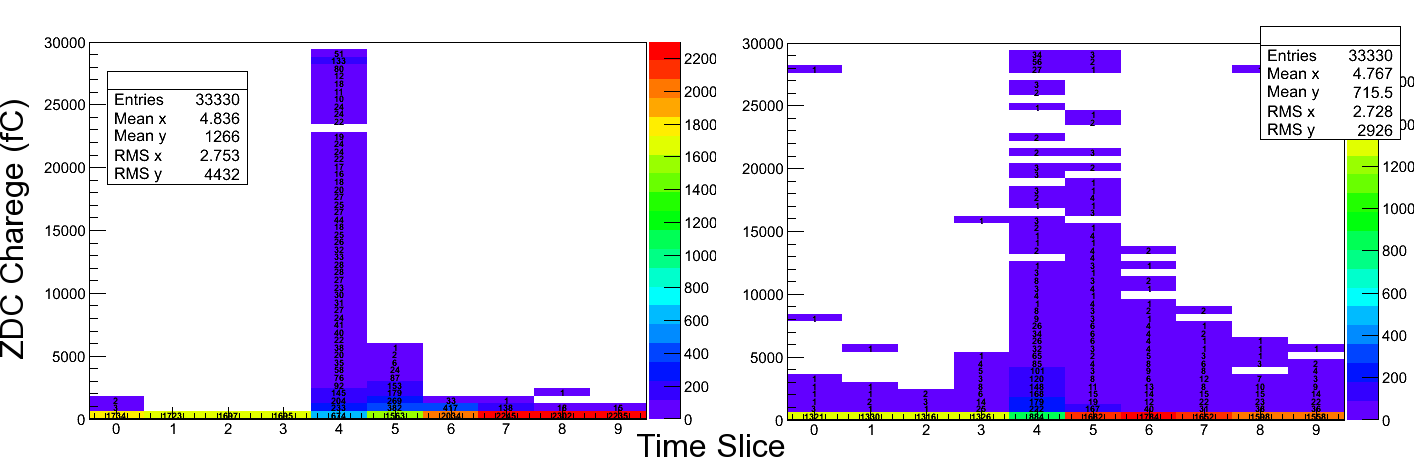
\includegraphics[width=\textwidth]{zdcPulseShape}
        \caption{Average ZDC pluse shape is plotted as the charge as a function
          of time slice for the first hadronic from ZDC$^{-}$ (left) and 
          ZDC$^{+}$ (right).}
        \label{fig:zdcPulseShape}
      \end{figure}

      The ZDC signal sits on top of a low frequency noise pedestal. 
      Over the time scale of 250 ns, this low frequency noise signal appears
        as a constant that shifts randomly from event to event.
      The contribution from this noise is therefore measured event by event
        in order to subtract it.
      Time slice 5 is used for this purpose.

      Time slices 1 and 2 could also be used to estimate the low frequency 
        noise.
      However because the noise fluctuates to negative values of charge that 
        cannot be measured, these time slices can only provide a 
        measurement of the noise half the time. 
      By using time slice 5 which contains the falling tail of the signal, 
        the noise can be measured any time the signal raises significantly 
        above the noise.
      If the fraction of signal in time slice 4 and 5 are constant and
        the noise contributes the same value to both time slices, the 
        following formula is applicable:
      \begin{equation}
        Ts4 \propto (Ts4 + C) - ( Ts5 + C ) = Ts4 - R_{Ts5/Ts4}Ts4 
        = Ts4(1-R_{Ts5/Ts4}),
        \label{eq:ts4ish}
      \end{equation}
      where $Ts4$ is the signal contribution in time slice 4, $Ts5$ is the 
        signal contribution to time slice 5, $C$ is a random noise constant
        from the low frequency noise, and $R_{Ts5/Ts4}$ is the ratio between
        the signal contribution from time slice 5 over time slice 4.
      Fig.~\ref{fig:zdcTs4OvTs5VTs5} demonstrates the consistence of the 
        fraction and validates the unconventional method of using the falling 
        tail of the signal to estimate the low frequency noise. 
      By using time slice 5, the chances of measuring the noise are maximized. 
      Separating the signal from the noise is especially important because
        the ZDC signal for the one neutron peak sits near the noise at the 
        bottom of the ZDC dynamic range.
      \begin{figure}[!Hhbt]
        \centering
        $ \begin{array}{cc}
          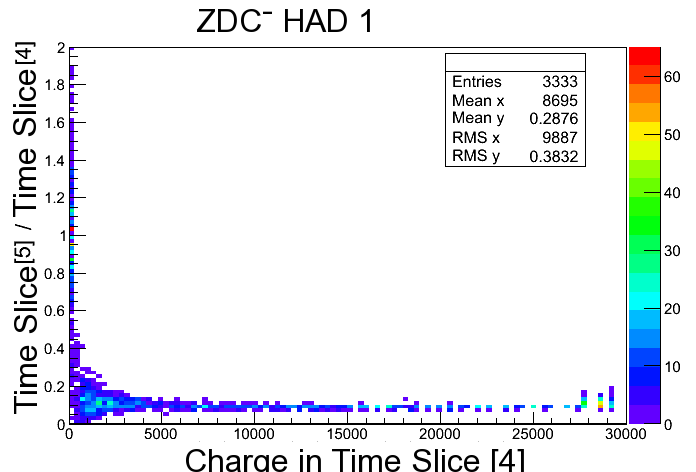
\includegraphics[width=.4\textwidth]{negTs5overTs4vts5} &
          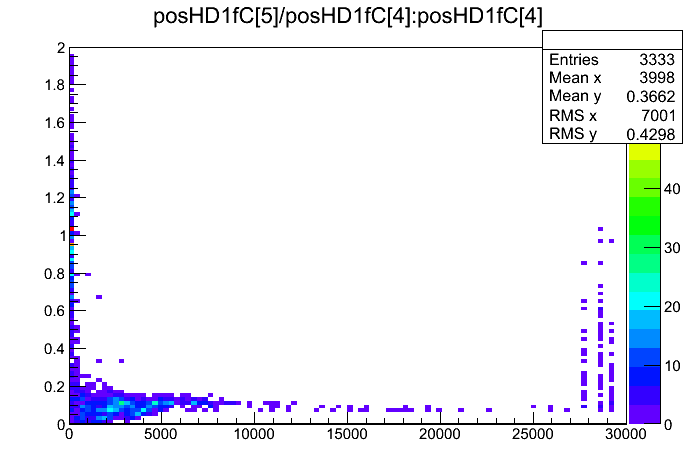
\includegraphics[width=.4\textwidth]{posTs5overTs4vts5}
        \end{array} $  
        \caption{ The fraction of signal in time slice 5 over time slice 4 
          as a function of the signal in time slice 5 in ZDC$^{-}$ (left) and 
          ZDC$^{+}$ (right).}
        \label{fig:zdcTs4OvTs5VTs5}
      \end{figure}
      
      To measure one signal value for ZDC$^{+}$ and one for ZDC$^{-}$, the 
        signals from each of the channels are combined.
      Channels from the EM section and HD section are combined first. 
      Only channels with signal above zero in time slice 5 and time slice 
        4 are included. 
      The EM section of the calorimeter is more densely packed with optical 
        fibers and therefore has a higher gain relative to the HAD section. 
      To account for this, the combination of EM channels is weighted with
        a factor of 0.1 to match the HAD channel gains.
      The value for each side of the ZDC's signal is given by the sum of the 
        HAD channel combination and weighted EM channel combination.
      It is this signal, one for ZDC$^{+}$ and one for ZDC$^{-}$, 
        which is plotted in Fig.~\ref{fig:zdcM2Fit} to measure the neutron 
        thresholds.

    \subsection{Determination of the one neutron thresholds}
      The ZDC thresholds used to establish the various break-up modes were 
        measured from zero bias data.
      By using this dataset, the neutron spectrum does not contain a trigger 
        bias. 
      Zero bias trigger required that both beams were present in CMS.
      This does, however, include a significant electronic noise contribution due
        to events where no neutrons are emitted in the direction of the ZDC.

      To determine the thresholds for one and multiple neutrons, the ZDC$^{+}$ 
        and ZDC$^{-}$ spectra were fit.
      Four Gaussian functions were combined to fit the spectra. 
      The electronic noise was fit to a Gaussian around zero.
      The one, two, and three neutron peaks are fit to Gaussians that are 
        successively broader.
      The mean of each peak was initially set to multiples of the mean of the 
        one neutron peak. 
      \begin{figure}[!Hh]
        \centering
        $ 
          \begin{array}{cc}
            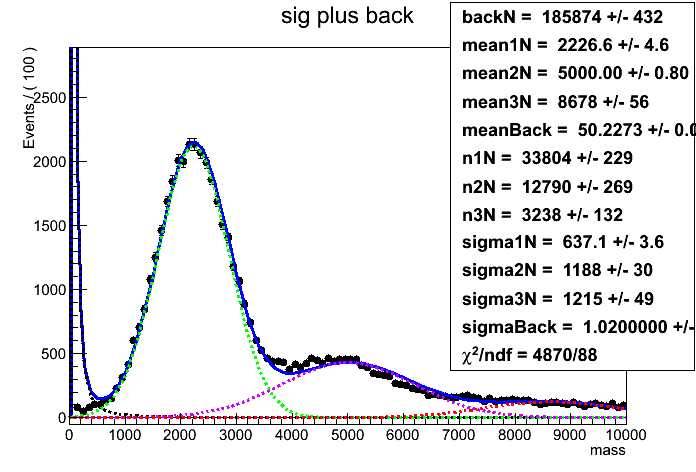
\includegraphics[width=0.45\textwidth]{zdcFit45Neg} &
            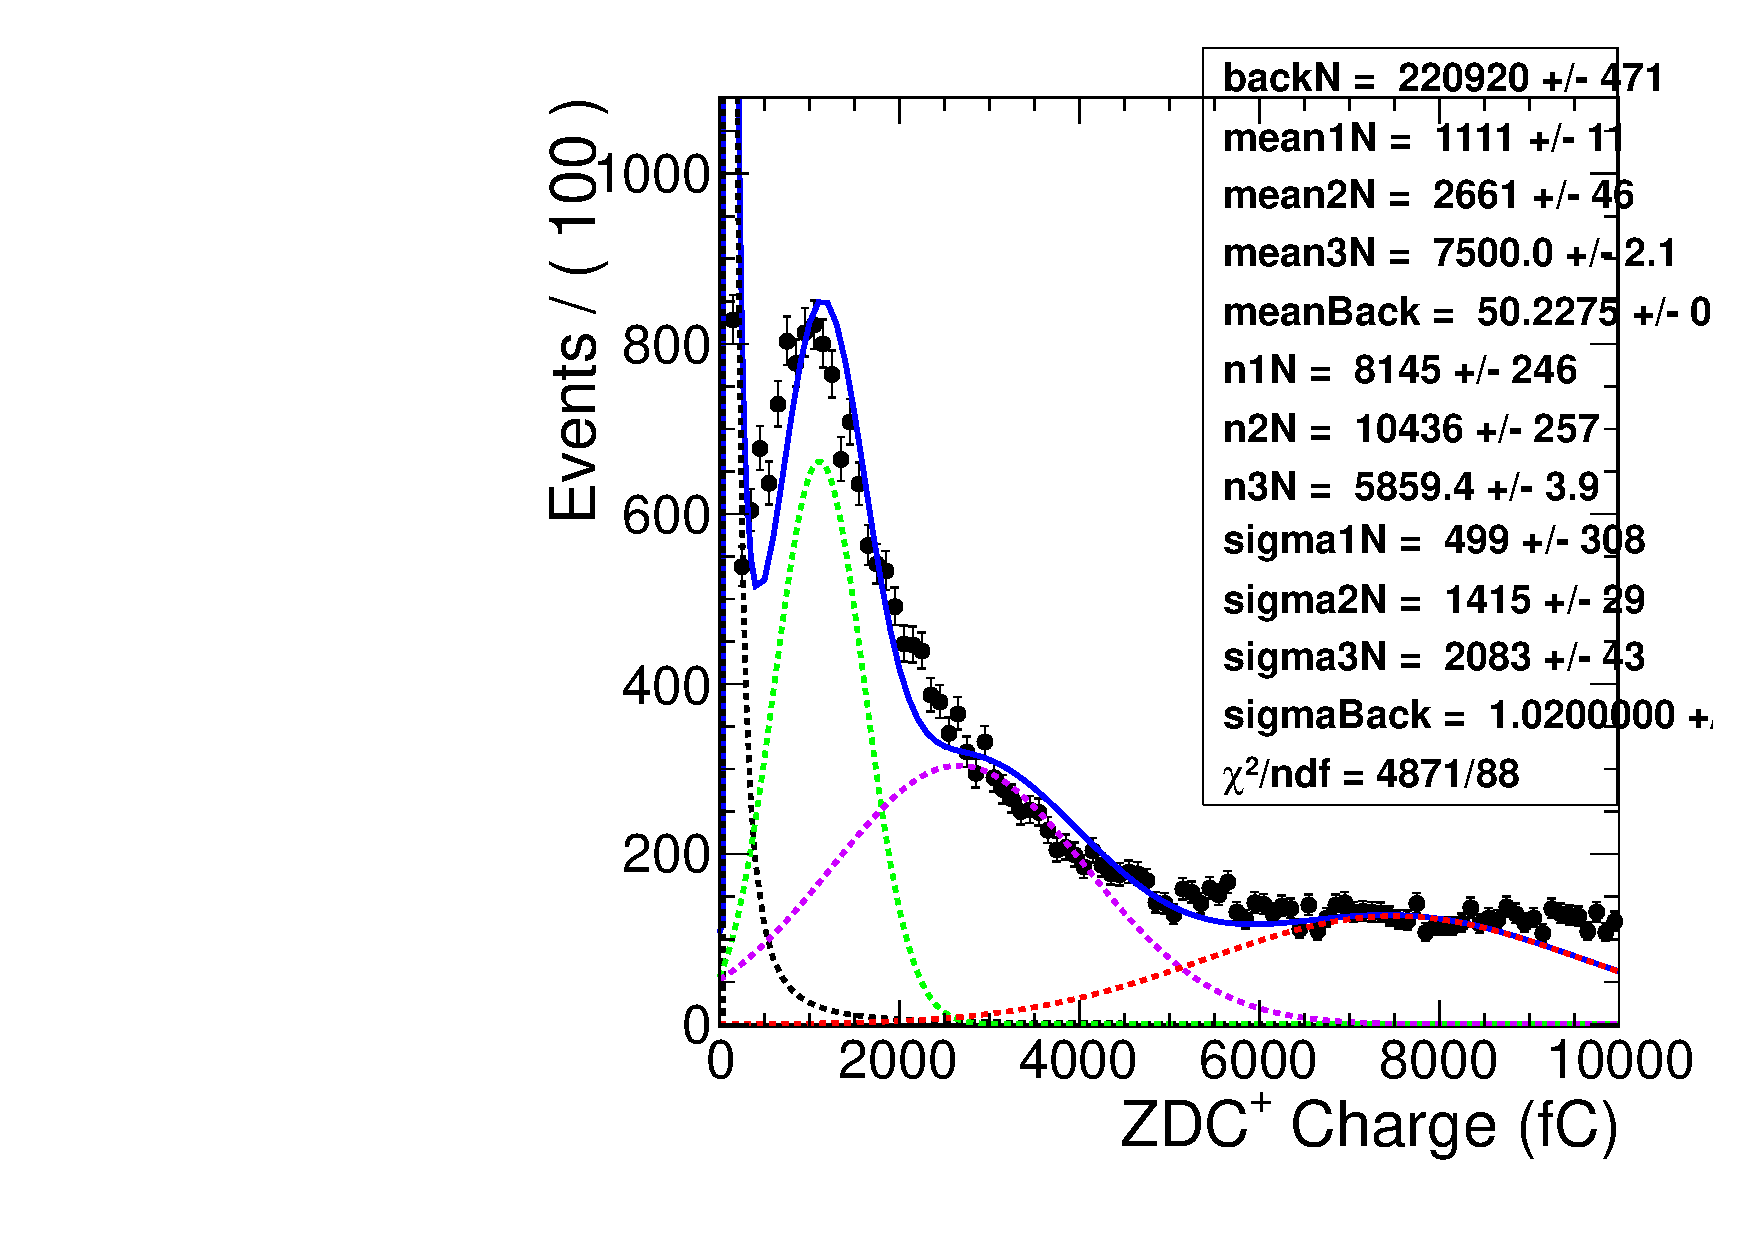
\includegraphics[width=0.45\textwidth]{zdcFit45Pos}
          \end{array} 
        $
        \caption{Fit to the signal spectra for ZDC$^{-}$ (left) and ZDC$^{+}$ 
          (right)}
        \label{fig:zdcM2Fit}
      \end{figure}
      The threshold for a neutron in the ZDC was taken from the fits in 
        Fig.~\ref{fig:zdcM2Fit}.
      Any signal greater 2$\sigma$ below the mean of the one neutron peak was 
        considered signal.
      Any signal greater than 2$\sigma$ above was considered multiple 
        neutrons.
      In this way the single neutron break up modes could be separated from the
        multiple neutron modes.

      Several of the break-up mode calculations that have been done involve
        single sided configurations where neutrons are present on one side
        of the interaction point and not the other.
      To identify signal consistent with noise, noise distributions for the 
        combined EM sections and the combined HAD sections were measured.
      The beams are only made to collide every 200 ns. 
      In Fig.~\ref{fig:zdcPulseShape} higher than average signal can be seen
        in the 0th time slice, which precedes the main signal time slice 
        time slice 4 by 200 ns. 
      This is due to events where activity was present in the ZDC for 
        two consecutive collisions.
      Time slices 1 and 2, however, occurred between collisions.
      These time slices were used to estimate the noise spectrum.
      \begin{figure}[!Hhbt]
        \centering
        $ \begin{array}{cc}
          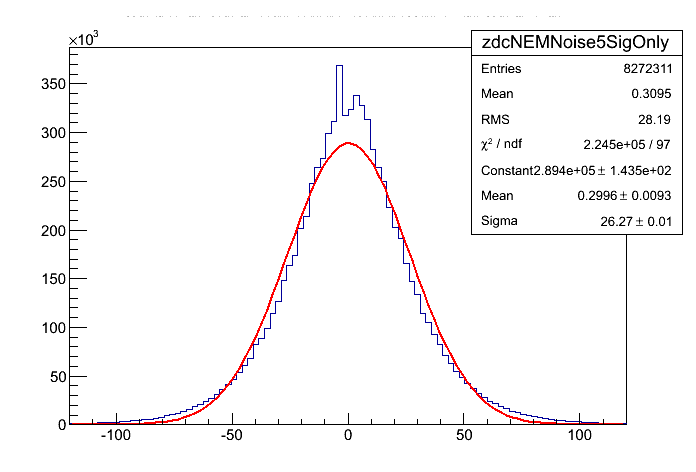
\includegraphics[width=.45\textwidth]{zdcNegEMNoiseFromZBNoCor} & 
          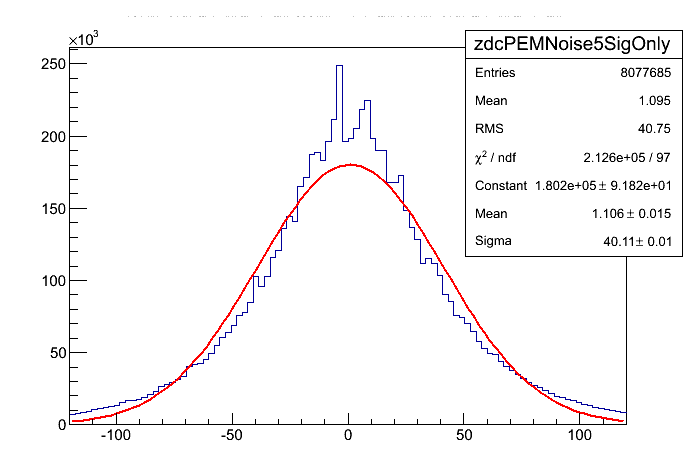
\includegraphics[width=.45\textwidth]{zdcPosEMNoiseFromZBNoCor} \\
          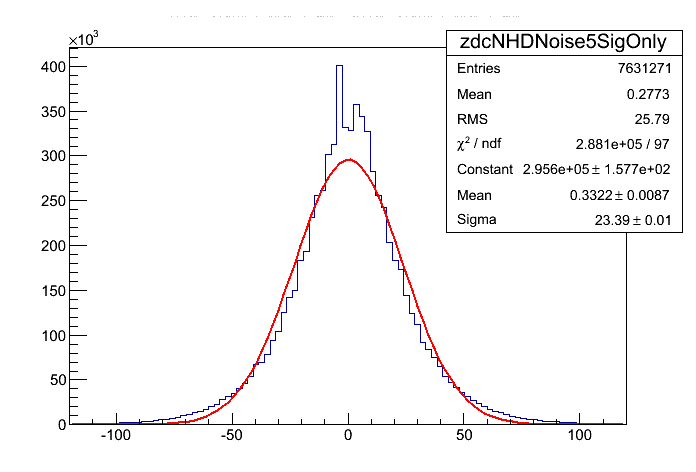
\includegraphics[width=.45\textwidth]{zdcNegHDNoiseFromZB} &
          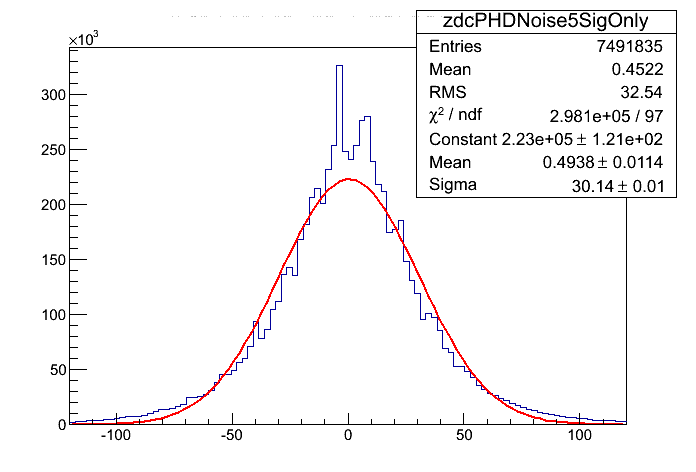
\includegraphics[width=.45\textwidth]{zdcPosHDNoiseFromZB}
        \end{array} $
        \caption{ZDC noise spectra from ZDC$^{-}$ EM section (upper left), 
          ZDC$^{+}$ EM section (upper right), ZDC$^{-}$ HAD section (lower left), 
          and ZDC$^{+}$ HAD section (lower right).}
        \label{fig:zdcNoiseSpectra}
      \end{figure}

      Fig~\ref{fig:zdcNoiseSpectra} shows the noise spectrum for each of the 
        EM and HAD sections for the two sides of the ZDC. 
      As with the signal measurements, the low frequency noise pedestal is 
        subtracted event by event by subtracting time slice 2 from time slice
        one before the channel signals are combined for each section.
      A side is considered consistent with noise if both HAD section and EM 
        section signal measurements from the signal method involving time slice
        4 and time slice 5 are lower than 2 sigma below the mean in 
        Fig.~\ref{fig:zdcNoiseSpectra}.
      With the single neutron, multi-neutron, and noise thresholds established,
        the contributions to the various break-up modes were estimated and 
        compared to theory. 


  \section{\label{sec:sigEx} Signal extraction}
    After all event selection cuts, the coherent \JPsi{}, incoherent \JPsi{},
      and photon-photon process all contribute to the remaining events.
    Each process must be separated from the final mix.
    To achieve this, the invariant mass and \pt{} distributions are used 
      to distinguish between the three processes. 
    The photon-photon process is extended in invariant mass whereas the 
      \JPsi{} is peak strongly near 3.1 GeV.
    In \pt{} the photon-photon and coherent process have similar 
      distributions, both peaked shapely below 0.1 GeV, whereas the incoherent 
      process is more broadly distributed across an interval extending to 
      nearly 1 GeV.
    The mass distribution was fit to separate the photon-photon process from
      the \JPsi{} process.
    The \pt{} distribution was used to separate the incoherent process from 
      the photon-photon process, and the coherent process. 
    In this way, a separate yield was extracted for all three processes. 
    
    The invariant mass distribution for opposite sign dimuons is shown in 
      Fig.~\ref{fig:massFit}. 
    A \JPsi{} signal is clearly visible together with tails at higher and
      lower mass due to the photon-photon process.
    A fit to the invariant mass distribution was done using a Gaussian
      to account for the \JPsi{} signal and a first order polynomial function 
      for the photon-photon process.
    The extracted number of \JPsi{} candidates from this fit includes all 
      \JPsi{}s in the mass window that passed the analysis cuts, i.e. both
      coherent and incoherent process contribute to yield from the mass
      fit.
    The \pt{} distribution is needed to separate the two different 
      contributions to the \JPsi{} peak. 

    \begin{figure}[!Hhtb]
      \centering
      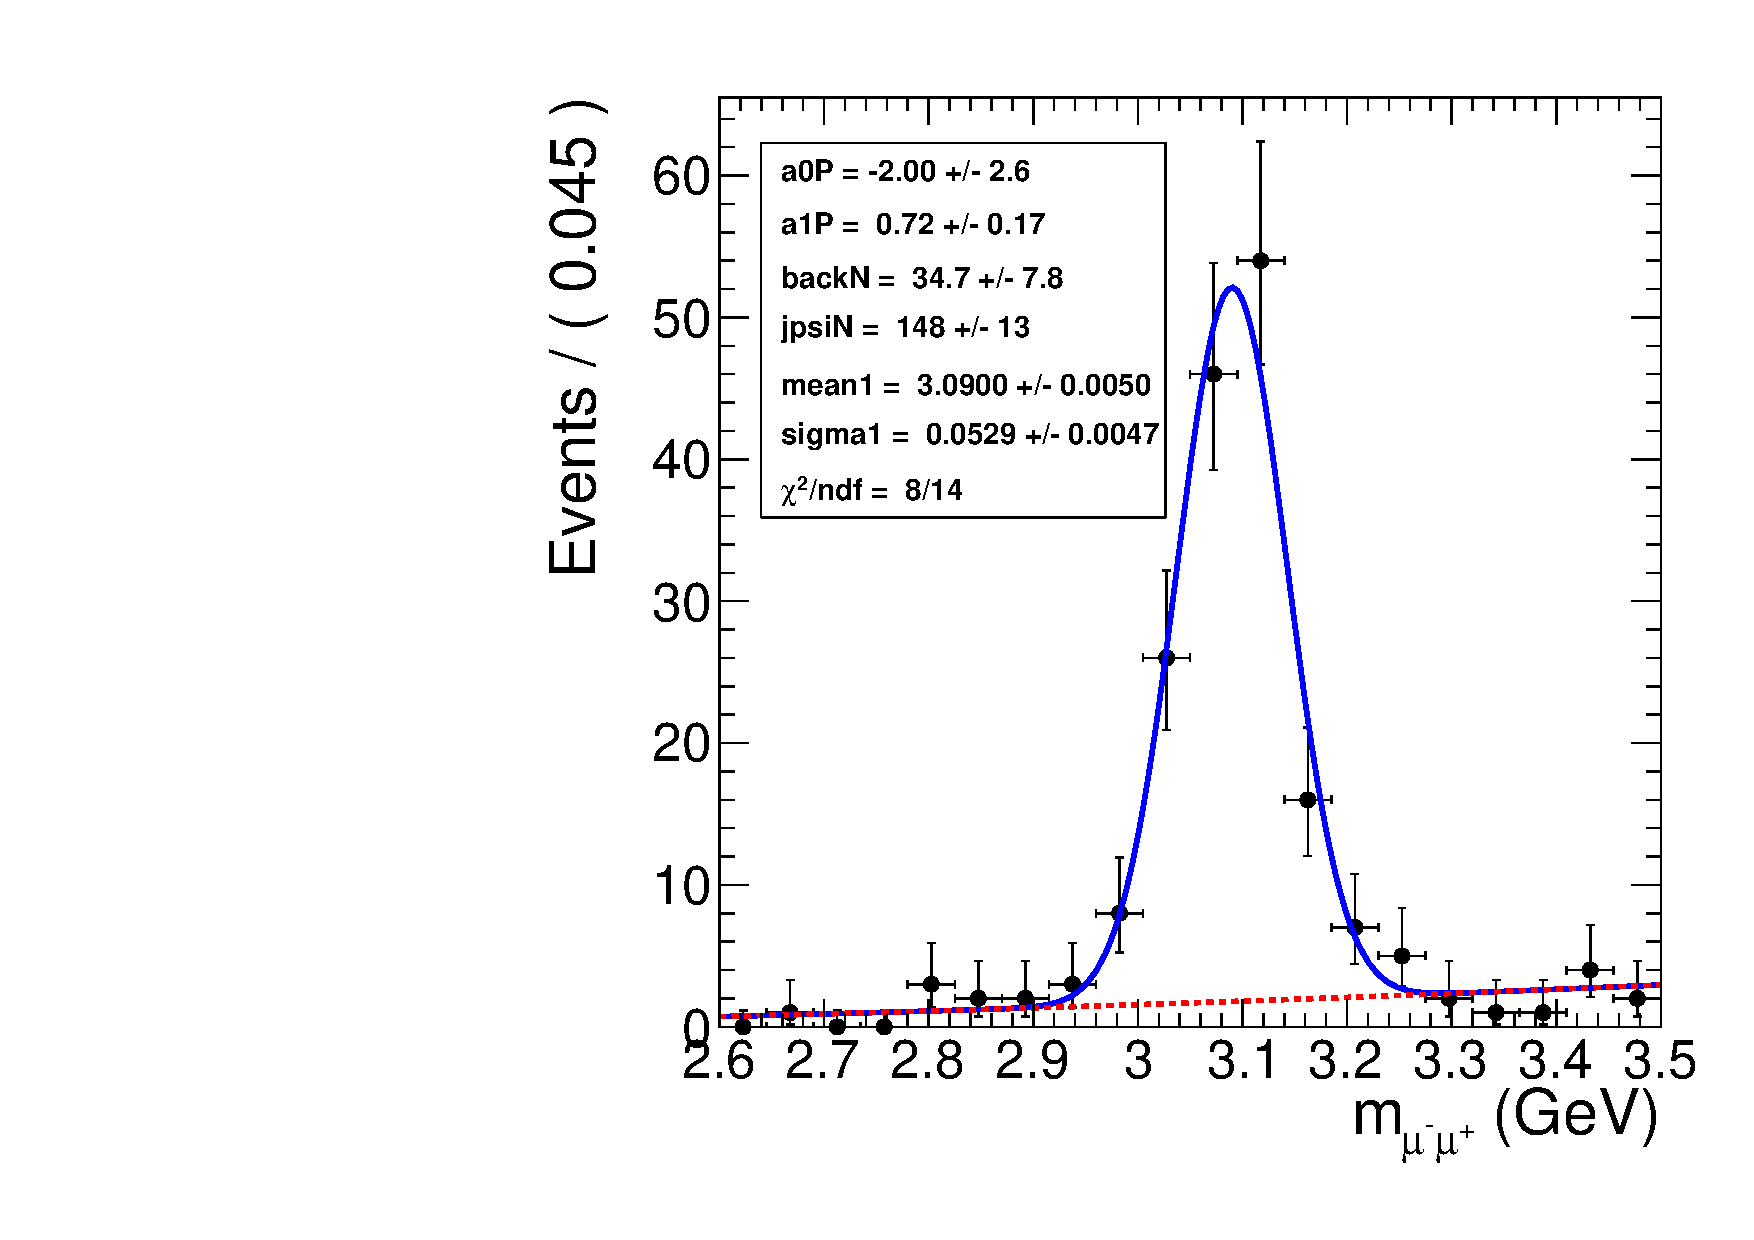
\includegraphics[width=.6\textwidth]{massFitSimple}
      \caption{Mass fit to \JPsi{} using Gaussian for the 
        signal and a first order polynomial for the photon-photon continuum}
      \label{fig:massFit}
    \end{figure}
   
    The same candidates from Fig.~\ref{fig:massFit} were plotted as a function
      of \pt{} in Fig.~\ref{fig:ptTemps}.
    The clear overlap of the coherent and photon-photon process, and the 
      clear separation of these two lower \pt{} processes from the incoherent
      process is apparent.
    The shape of the \pt{} distribution for the coherent, incoherent, and 
      photon-photon process are taken from the final output of MC after
      applying all analysis cuts. 
    To obtain the yields for each of the three process, the \pt{} 
      distribution was fit to the three templates.
    In Fig.\ref{fig:ptTemps}, the yield parameters that were fit were left
      unconstrained for all three process.

    \begin{figure}[!Hhbt]
      \centering
      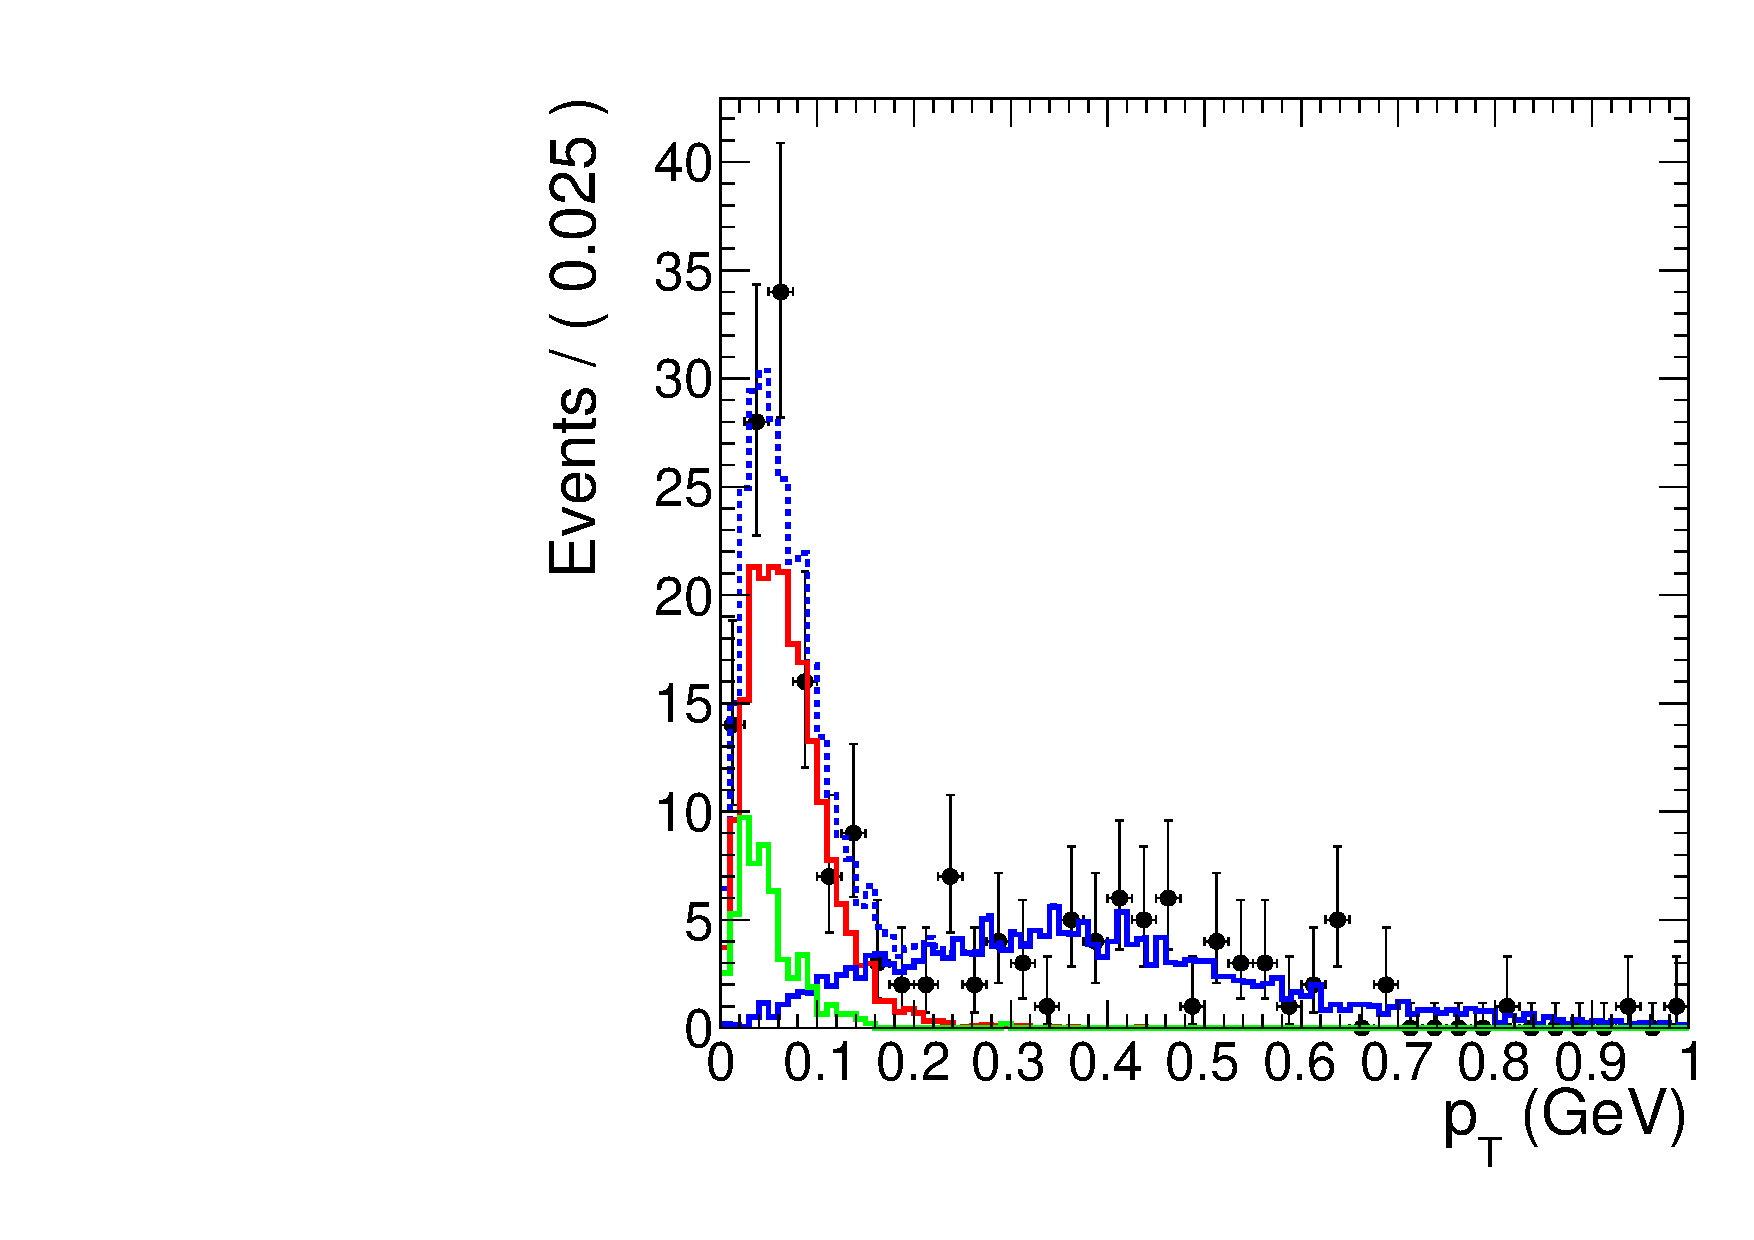
\includegraphics[width=.6\textwidth]{ptOnly}
      \caption{ Fit to MC \pt{} templates. }
      \label{fig:ptTemps}
    \end{figure}

    The shape of the photon-photon and coherent \JPsi{} process are very 
      similar in \pt{}.
    Accordingly, the contribution from the photon-photon process and the 
      coherent process are difficult to separate from the \pt{} distribution.
    The confidence contours in Fig.~\ref{fig:ptOnlyCor} from the template fit
      in Fig.~\ref{fig:ptTemps} demonstrate the strong anti-correlation 
      between the coherent yield parameter, $nCo$, and the yield parameter 
      for the photon-photon process, $nGamma$.
    Because of the anti-correlation, the statistical uncertainty on $nCo$ and 
      $nGamma$ from the fit are larger than $\sqrt{nCo}$ and $\sqrt{nGamma}$
      expected from Poisson statistics. 
    The information from the invariant mass and \pt{} distributions were
      combined to break this correlation. 
    Through this combination, the contribution to the final yield from 
      the three process was measured.

    \begin{figure}[!Hhbt]
      \centering
      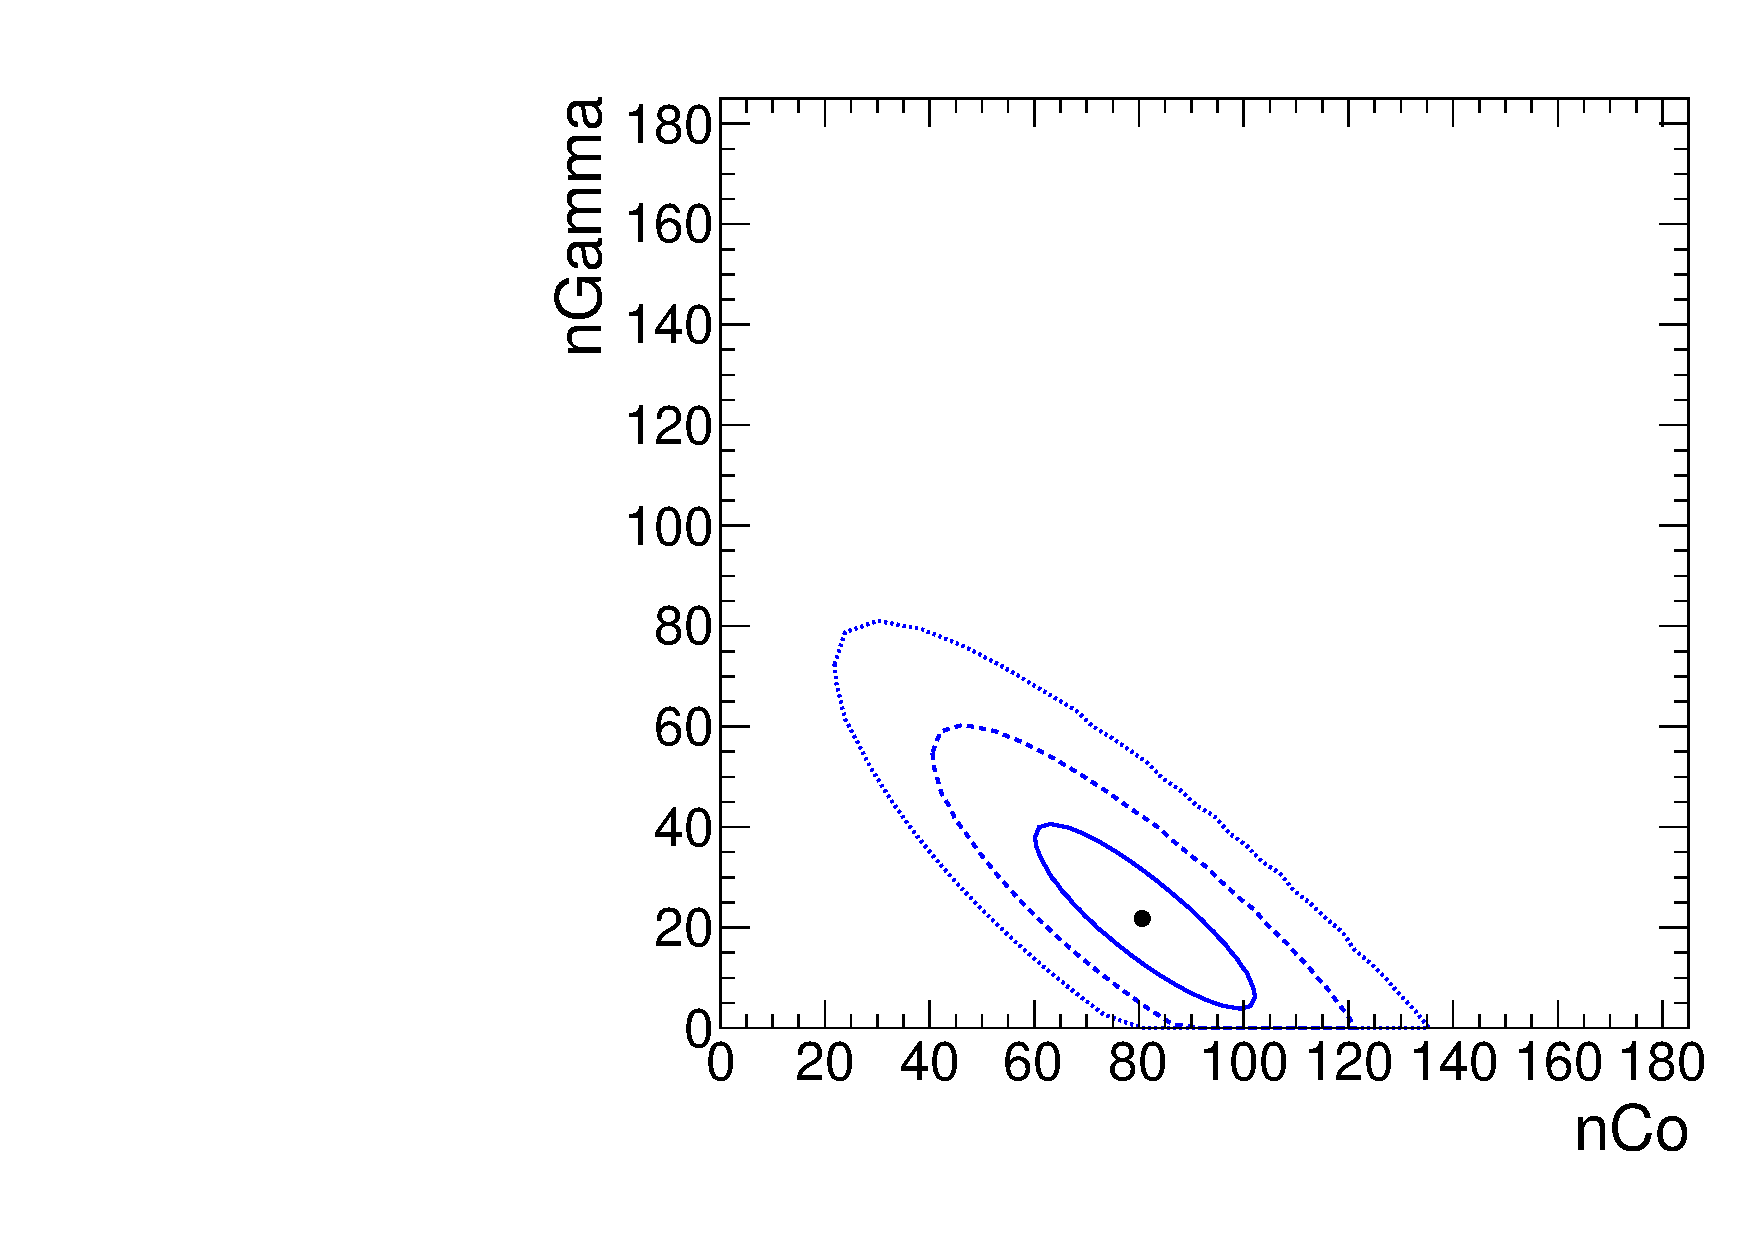
\includegraphics[width=.6\textwidth]{nCoNGammaCorPtOnly}
      \caption{68\%, 95\%, and 99\% confidence contours from the \pt{} 
        template fit. }
      \label{fig:ptOnlyCor}
    \end{figure}

    To utilize the mass fits ability to distinguish the photon-photon process 
      from the coherent and incoherent process all while utilizing the \pt{}
      fits ability to separate the coherent and photon-photon processes from 
      the incoherent, a simultaneous fit to the mass spectrum and \pt{} 
      spectrum was preformed.
    Fig.~\ref{fig:simFitMassPtGauss} shows the result of the simultaneous fit.
    The simultaneous fit forces the parameter $nGamma$ to both describe the 
      photon-photon continuum present in the side bands of the \JPsi{} mass 
      peak as well the photon-photon contribution to the low-\pt{} part of 
      the \pt{} spectrum.
    In addition, the \JPsi{} yield from the mass fit is forced to equal the
      contribution from the incoherent and coherent process in the 
      fit to the \pt{} distribution. 
    In this way, the correlation between the yield parameters was broken, and 
      the contribution from the three process were made independent of each 
      other.
      
    \begin{figure}[!Hhbt]
      \centering
      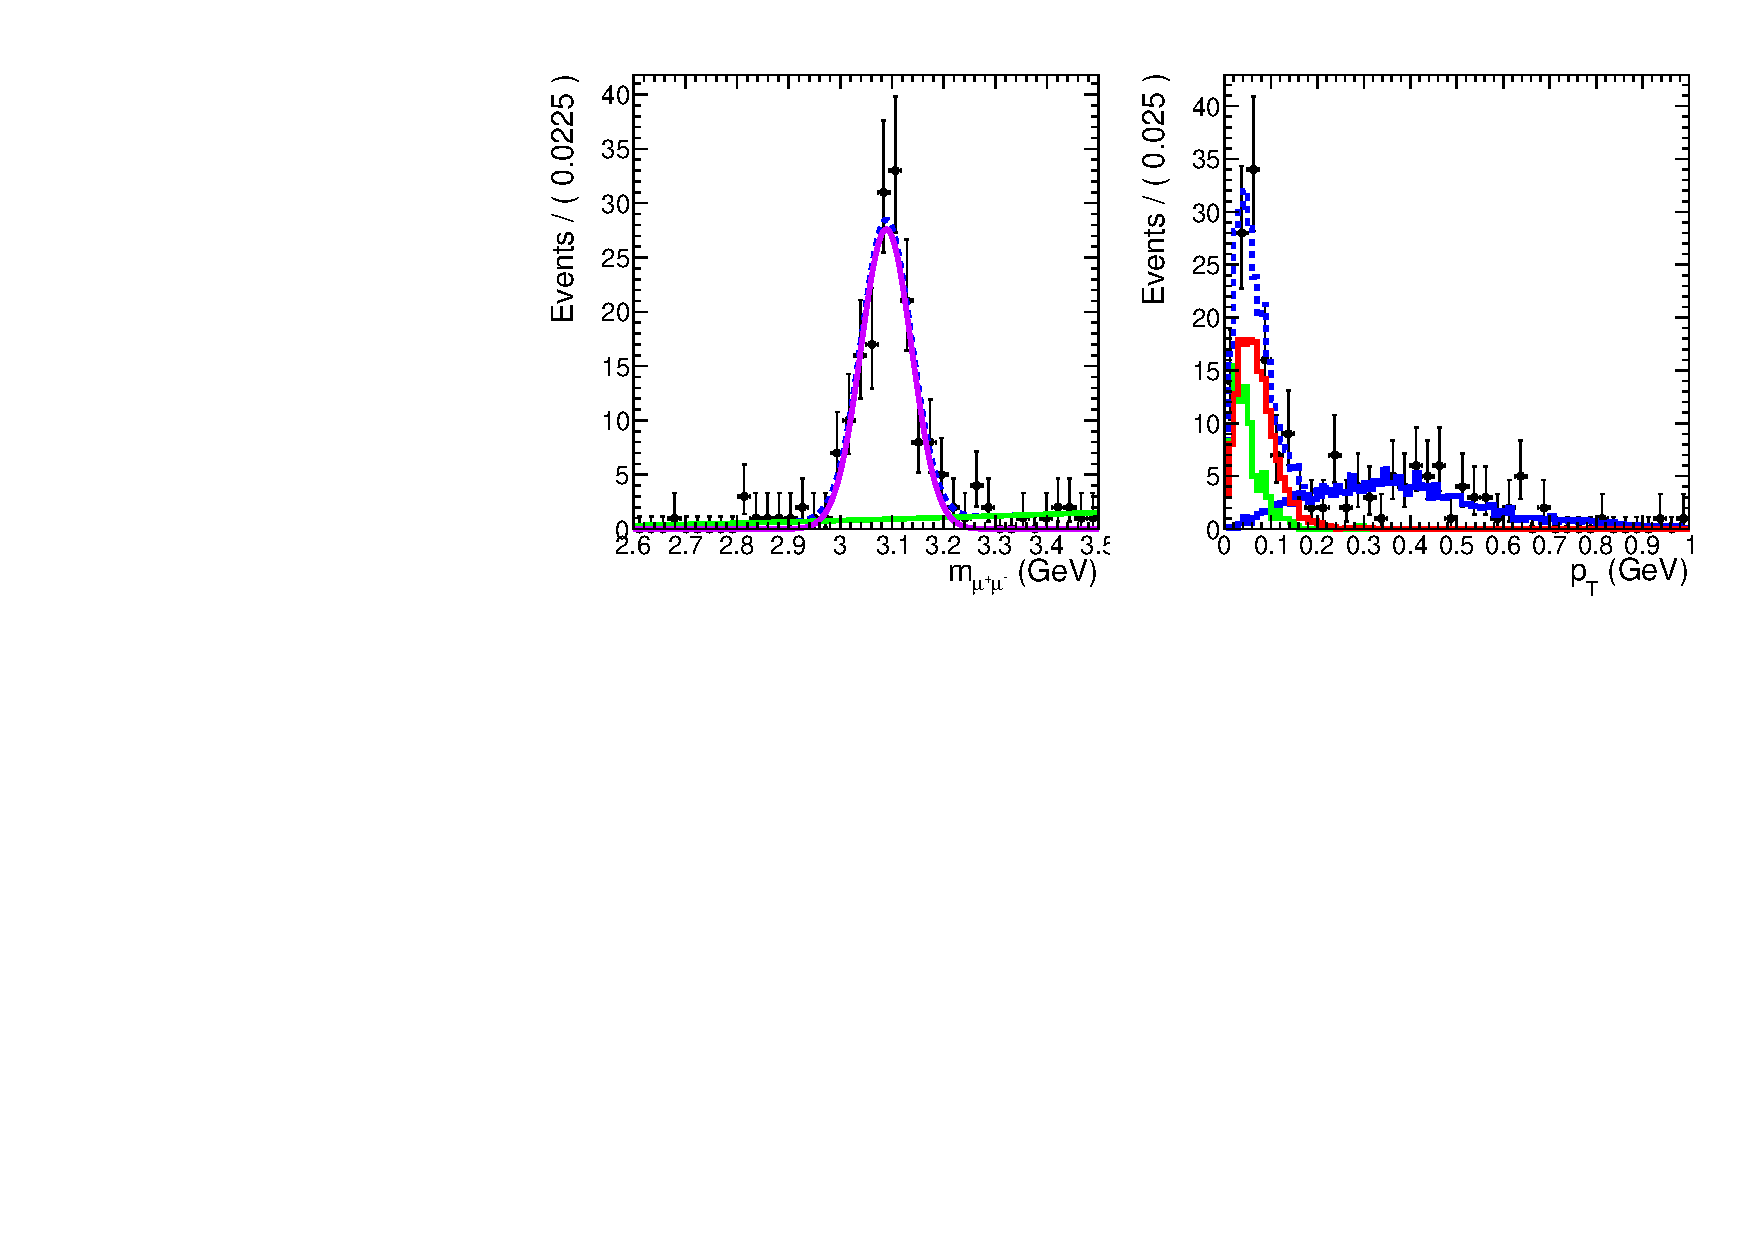
\includegraphics[width=0.9\textwidth]{ptMassSimGaussLine}
      \caption{Simultaneous fit to the mass and \pt{} spectra.}
      \label{fig:simFitMassPtGauss}
    \end{figure}

    The ambiguity between the coherent and incoherent processes in the mass fit
      and the ambiguity between the coherent and the photon-photon process was 
      over come through used of the simultaneous fit.
    Fig.~\ref{fig:simGaussCor} shows the confidence contours for $nCo$ and 
      $nGamma$ from the simultaneous fit in Fig.~\ref{fig:simFitMassPtGauss}.  
    The slope of the confidence contours in Fig.~\ref{fig:simGaussCor} 
      is noticeably closer to 0 than the apparent negative slope in 
      Fig.~\ref{fig:ptOnlyCor}.
    The contours for the simultaneous fit are also reduced compared to 
      Fig.~\ref{fig:ptOnlyCor} with widths in $nCo$ and $nGamma$ similar to 
      those expected from Poison statistics. 
    From the simultaneous fit, reasonable statistical errors were obtained 
      along with the yields for the three processes. 

    \begin{figure}[!Hhbt]
      \centering
      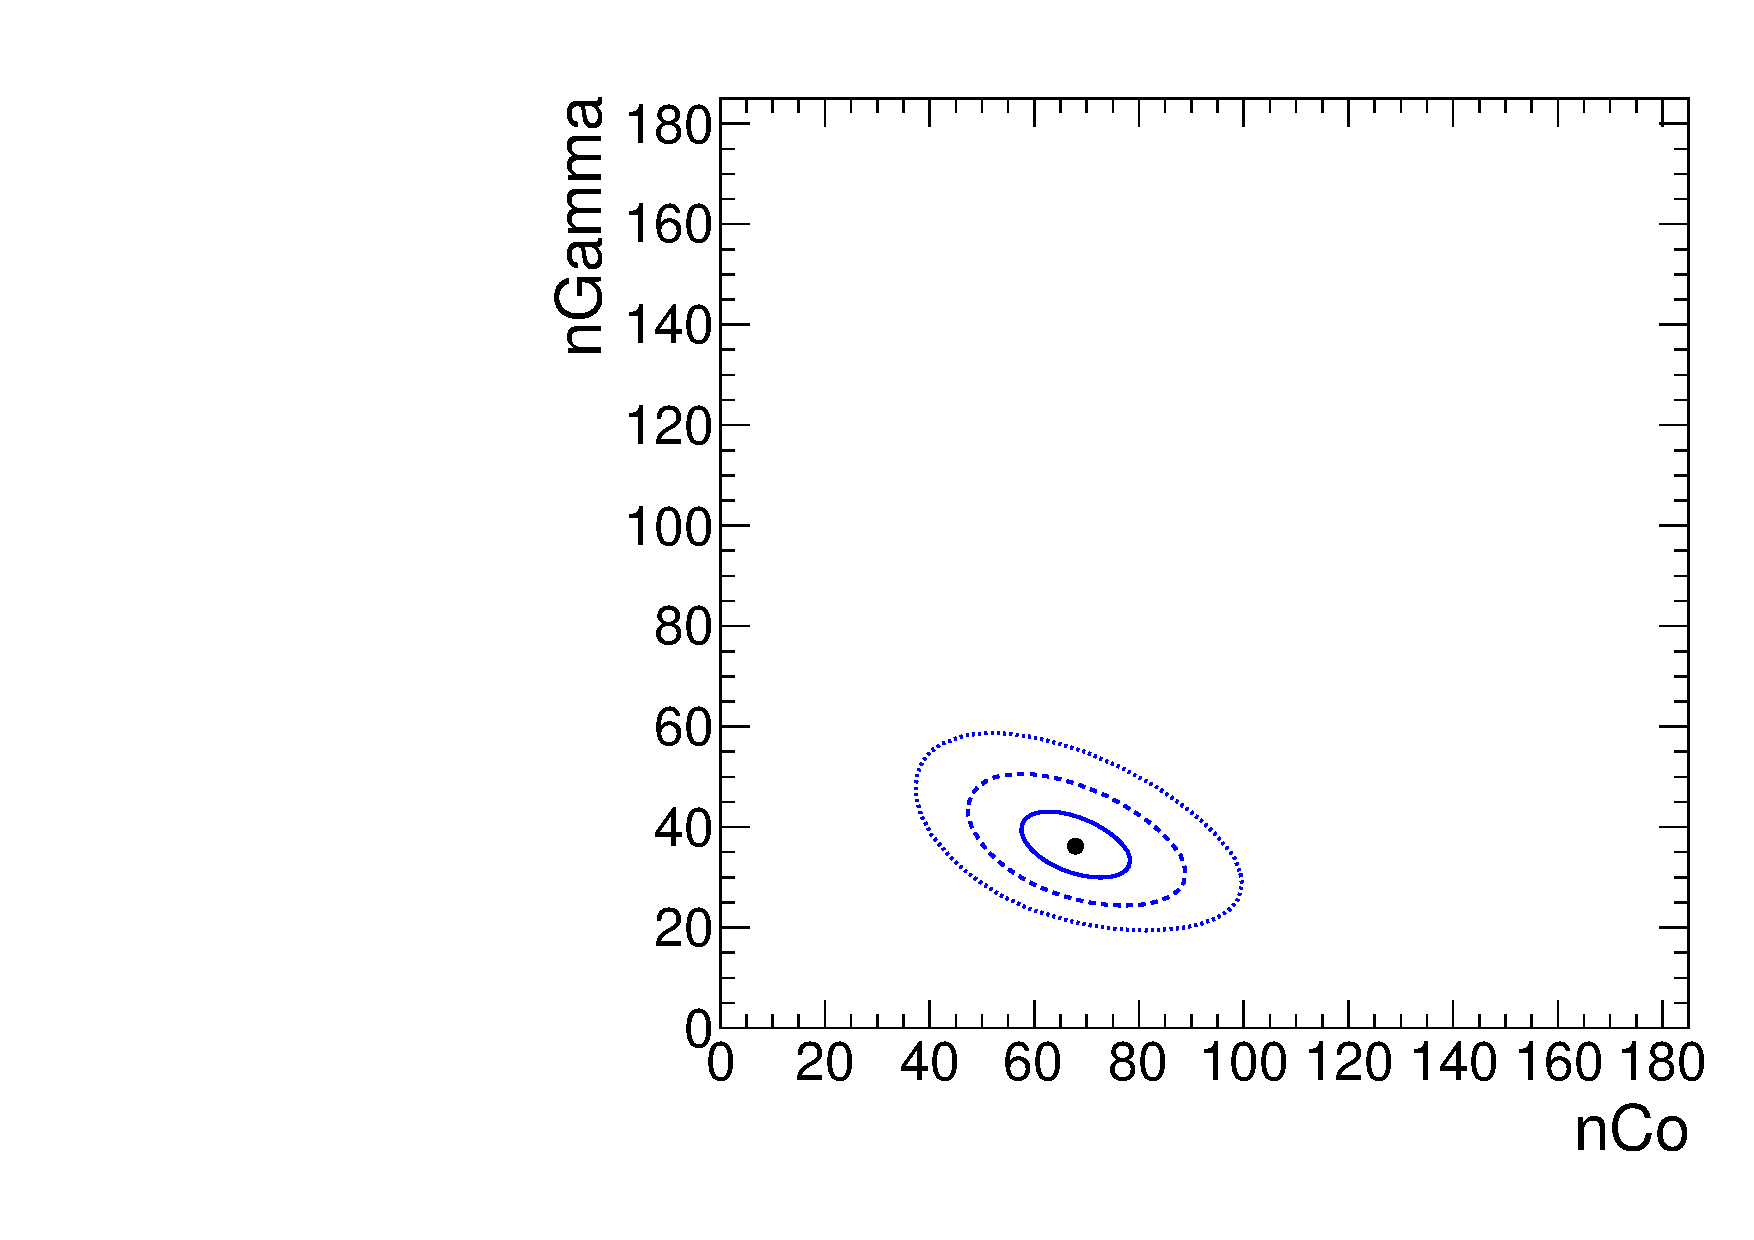
\includegraphics[width=0.6\textwidth]{nCoNGammaCorPtMass}
      \caption{68\%, 95\%, and 99\% confidence contours from the 
        simultaneous fit. }
      \label{fig:simGaussCor}
    \end{figure}

  \section{\label{sec:effDet} Efficiency determination}
    \subsection{Muon efficiencies}
      The muon efficiencies are measured from MC and data.
      The MC based measurement accounts for the detector acceptance and the 
        efficiency of the muon quality discussed in 
        Section~\ref{sec:DataSetEvSel}.
      The trigger efficiencies were measured in data using the tag and probe 
      method \cite{cmsTnP}, which is discussed below. 

       CMS has a limited acceptance for \JPsi{}s, particularly in the case of 
        \JPsi{}s with low momentum like those produced in UPC events. 
      To measure the acceptance of CMS for \JPsi{}s, reconstructed dimuon 
        candidates were considered detectable if both reconstructed daughters 
        fell into a detectability region.
      This region was defined using the coherent \JPsi{} events obtained from 
        STARlight.
      The efficiency for reconstructing single muons $\varepsilon^{\mu}_{reco}$ 
        is defined by $\varepsilon^{\mu}_{reco} = \frac{N^{\mu}_{reco}}{N^{\mu}_{gen}}$, 
        where $N^{\mu}_{reco}$ is the number reconstructed muons obtained 
        after the full CMS detector simulation and that passed the standard
        muon quality cuts, and $N^{\mu}_{gen}$ is the number of generated 
        muons from STARlight.
      \begin{figure}[!Hhtb]
        \centering
          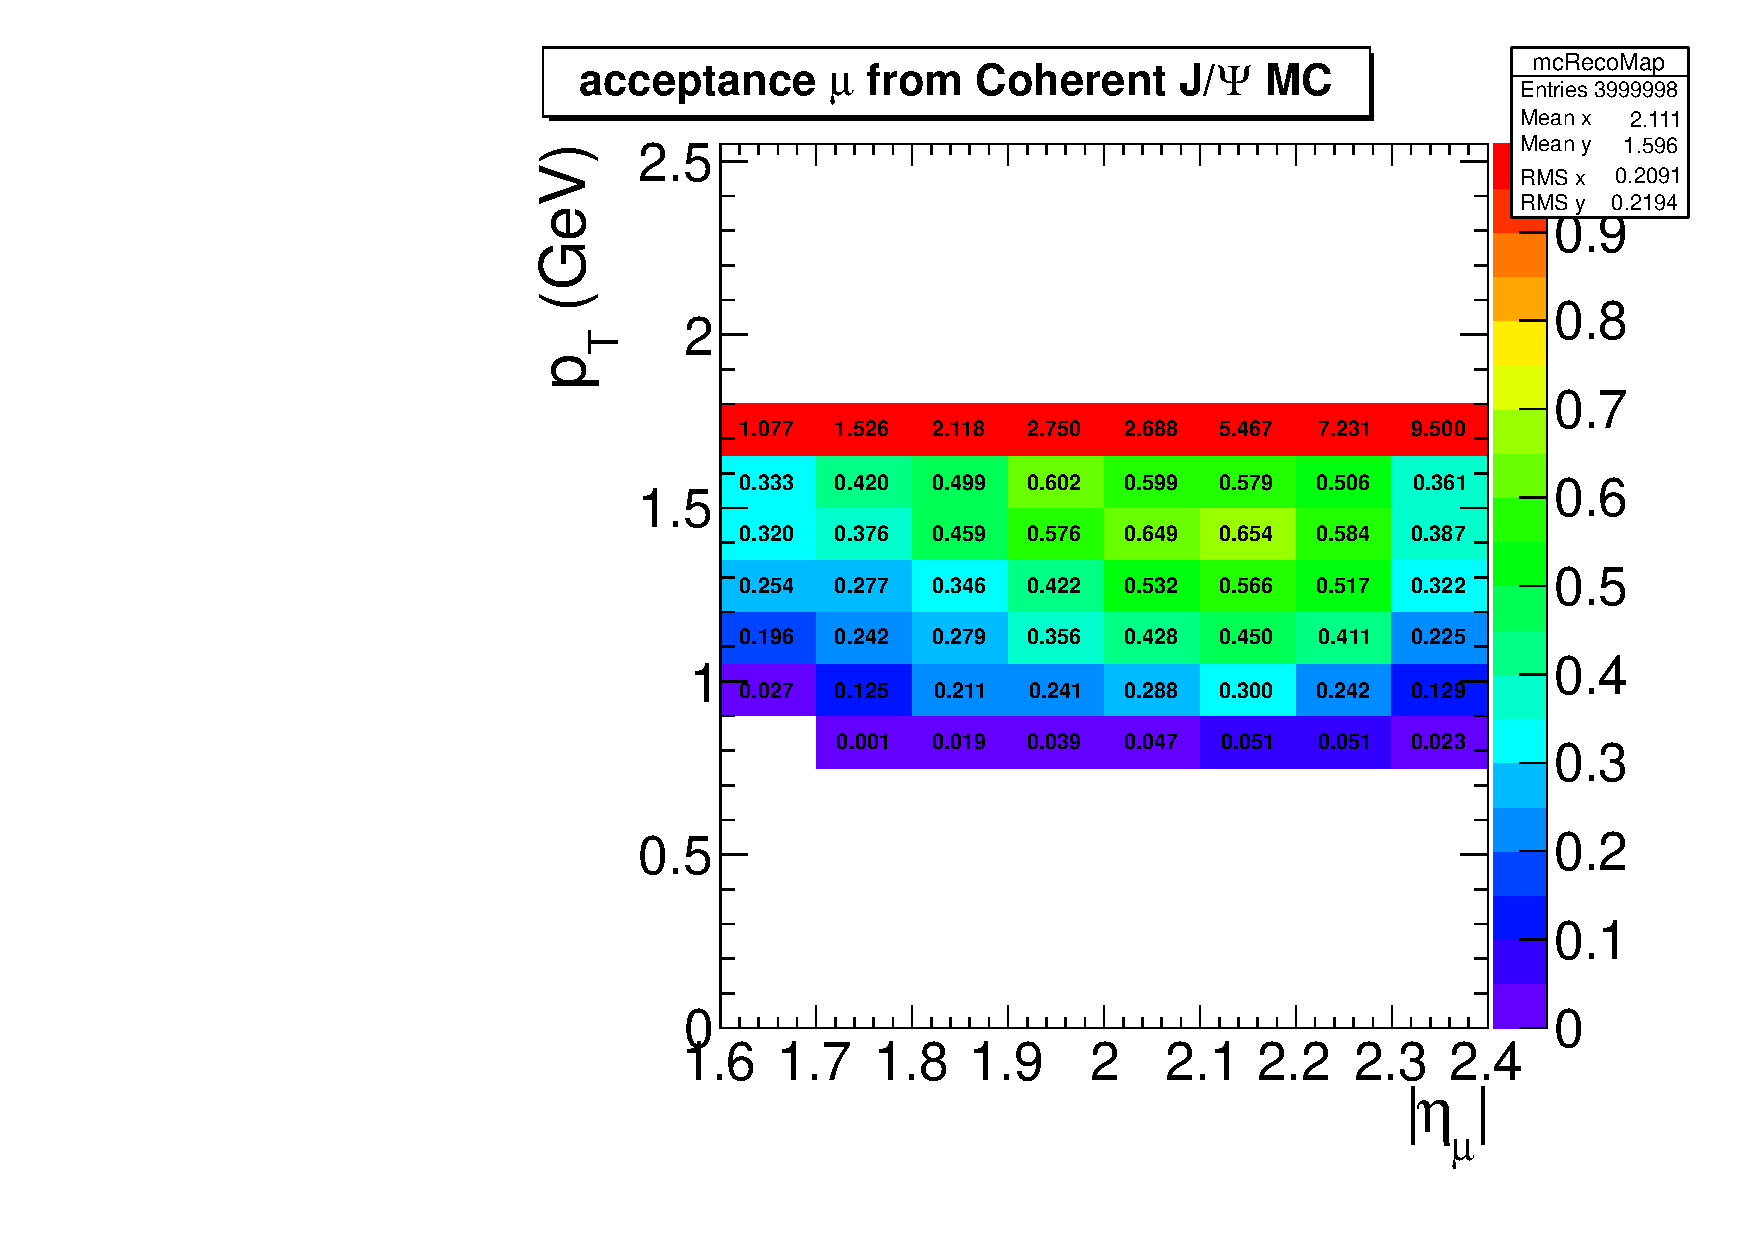
\includegraphics[width=.6\textwidth]{mcEffMaps/accMuJpCo} 
        \caption{ Muon daughter detectability from coherent \JPsi{}}
        \label{fig:muonDaughterDet}
      \end{figure}
      Fig.~\ref{fig:muonDaughterDet} shows the efficiency for reconstructing
        single muons from coherent \JPsi{} events.
      To avoid the edges of the detectors acceptance, all reconstructed muons 
        that fall into a (\pt{},$|\eta|$) bin that has an efficiency less 
        than 20\% were rejected thus defining the detectability region.
      The acceptance for reconstructing dimuons was calculated from MC
        using the following formula:
      \begin{equation}
        A=\frac{N_{det}(|y|,p_{T})}{N_{gen}(|y|,p_{T})},
        \label{eq:jpsiAccEq}
      \end{equation}
        where $N_{det}$ is the number of reconstructed dimuons where both 
        daughters fall into the detectability region, and $N_{gen}$ is the
        number of generated dimuons. 
      From Eq.~\ref{eq:jpsiAccEq}, the acceptance for \JPsi{} was calculated
        as a function of $|y|$, and \pt{} (see Fig.~\ref{fig:jpsiAcceptance}).
        \begin{figure*}[!Hhtb]
          \centering
          $ \begin{array}{cc}
            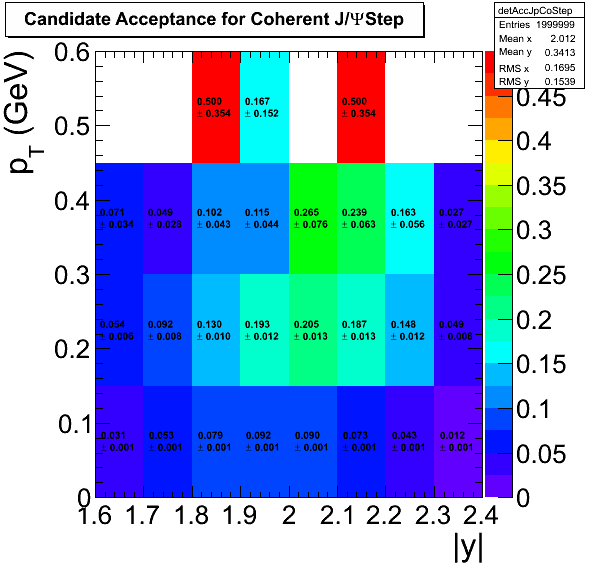
\includegraphics[width=.45\textwidth]{mcEffMaps/detAccJpCoStep} &
            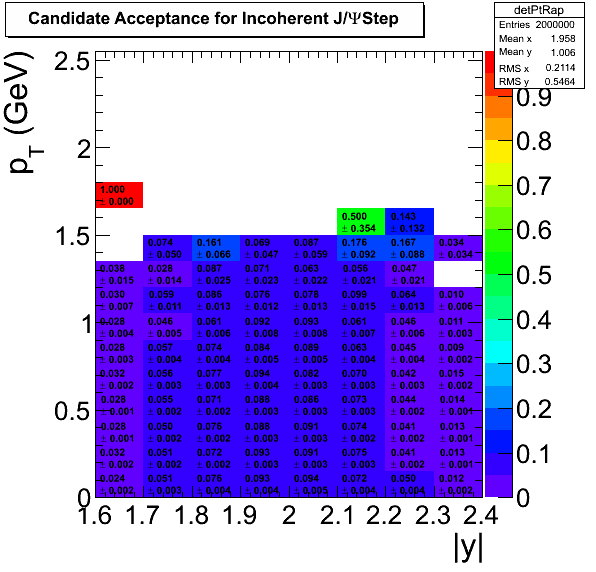
\includegraphics[width=.45\textwidth]{mcEffMaps/detAccJpInCoStep} \\
            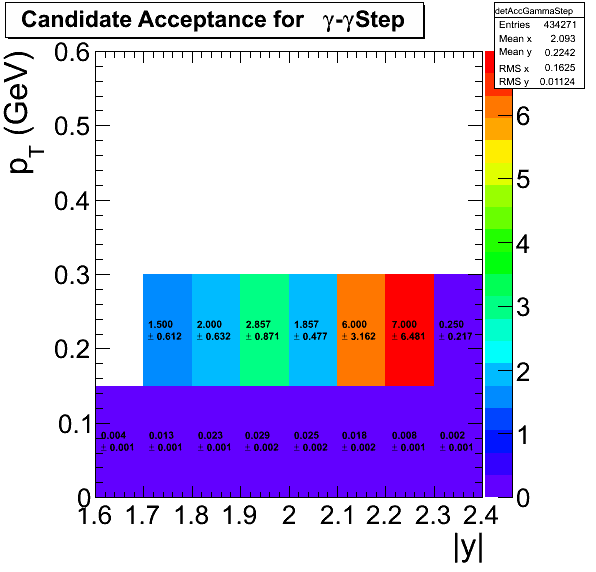
\includegraphics[width=.45\textwidth]{mcEffMaps/detAccGammaStep}
          \end{array} $
          \caption{Dimuon acceptance from coherent \JPsi{} (top left), incoherent 
            J$\psi$ (top right), and photon-photon interactions (lower).}
          \label{fig:jpsiAcceptance}
        \end{figure*}

      The tag and probe method is used to measure the trigger efficiency of 
        the muon daughters, which is a data driven approach. 
      In this method there are three categories of daughter muons. 
      \textit{Tag muons} are high quality muons.
      \textit{Passing probes} are reconstructed muons that match the muon trigger, 
        while \textit{failing probes} do not. 
      Each dimuon will have one daughter classified as a tag and the other
        as a probe.
      From here three invariant mass histograms are studied. 
      One histogram is created from all pairs. 
      The second comes from pairs where the probe is a passing probe.  
      The last histogram comes from pairs where the probe fails to fulfill
        the trigger, \textit{i.e.} the probe is a failing probe. 
      Because this depends on the \pt{} and $|\eta|$ of the probe, one set 
        of three histograms for each (\pt{},$|\eta|$) bin of the probe is 
        created.

      To extract the single muon trigger efficiency $\varepsilon^{\mu}_{trig}$, 
        each set of invariant mass histograms was simultaneously fitted. 
      The signal was fitted using a Crystal Ball function, and the background 
        was fitted to an exponential.
      The Crystal Ball parameters were simultaneously fitted to all three 
        histograms.
      The exponential function was fitted to the failing and passing probe 
        histograms separately.
      Because the background shapes are in principle different for the two 
        samples, the efficiency is driven by this difference. 

      To measure the trigger efficiency a tag is required to pass all muon
        quality cuts and matched to the trigger.
      The probe is required to pass all quality cuts. 
      A passing probe is a probe that is also matched to the trigger. 
      In this way, the tag leaves the probe unbiased by the trigger and the 
        efficiency can be measured by fitting the mass distribution.  

      Fig.~\ref{fig:tnpFitPlot} shows the fit of the three sets of pairs. 
      \begin{figure}[!Hh]
        \centering
        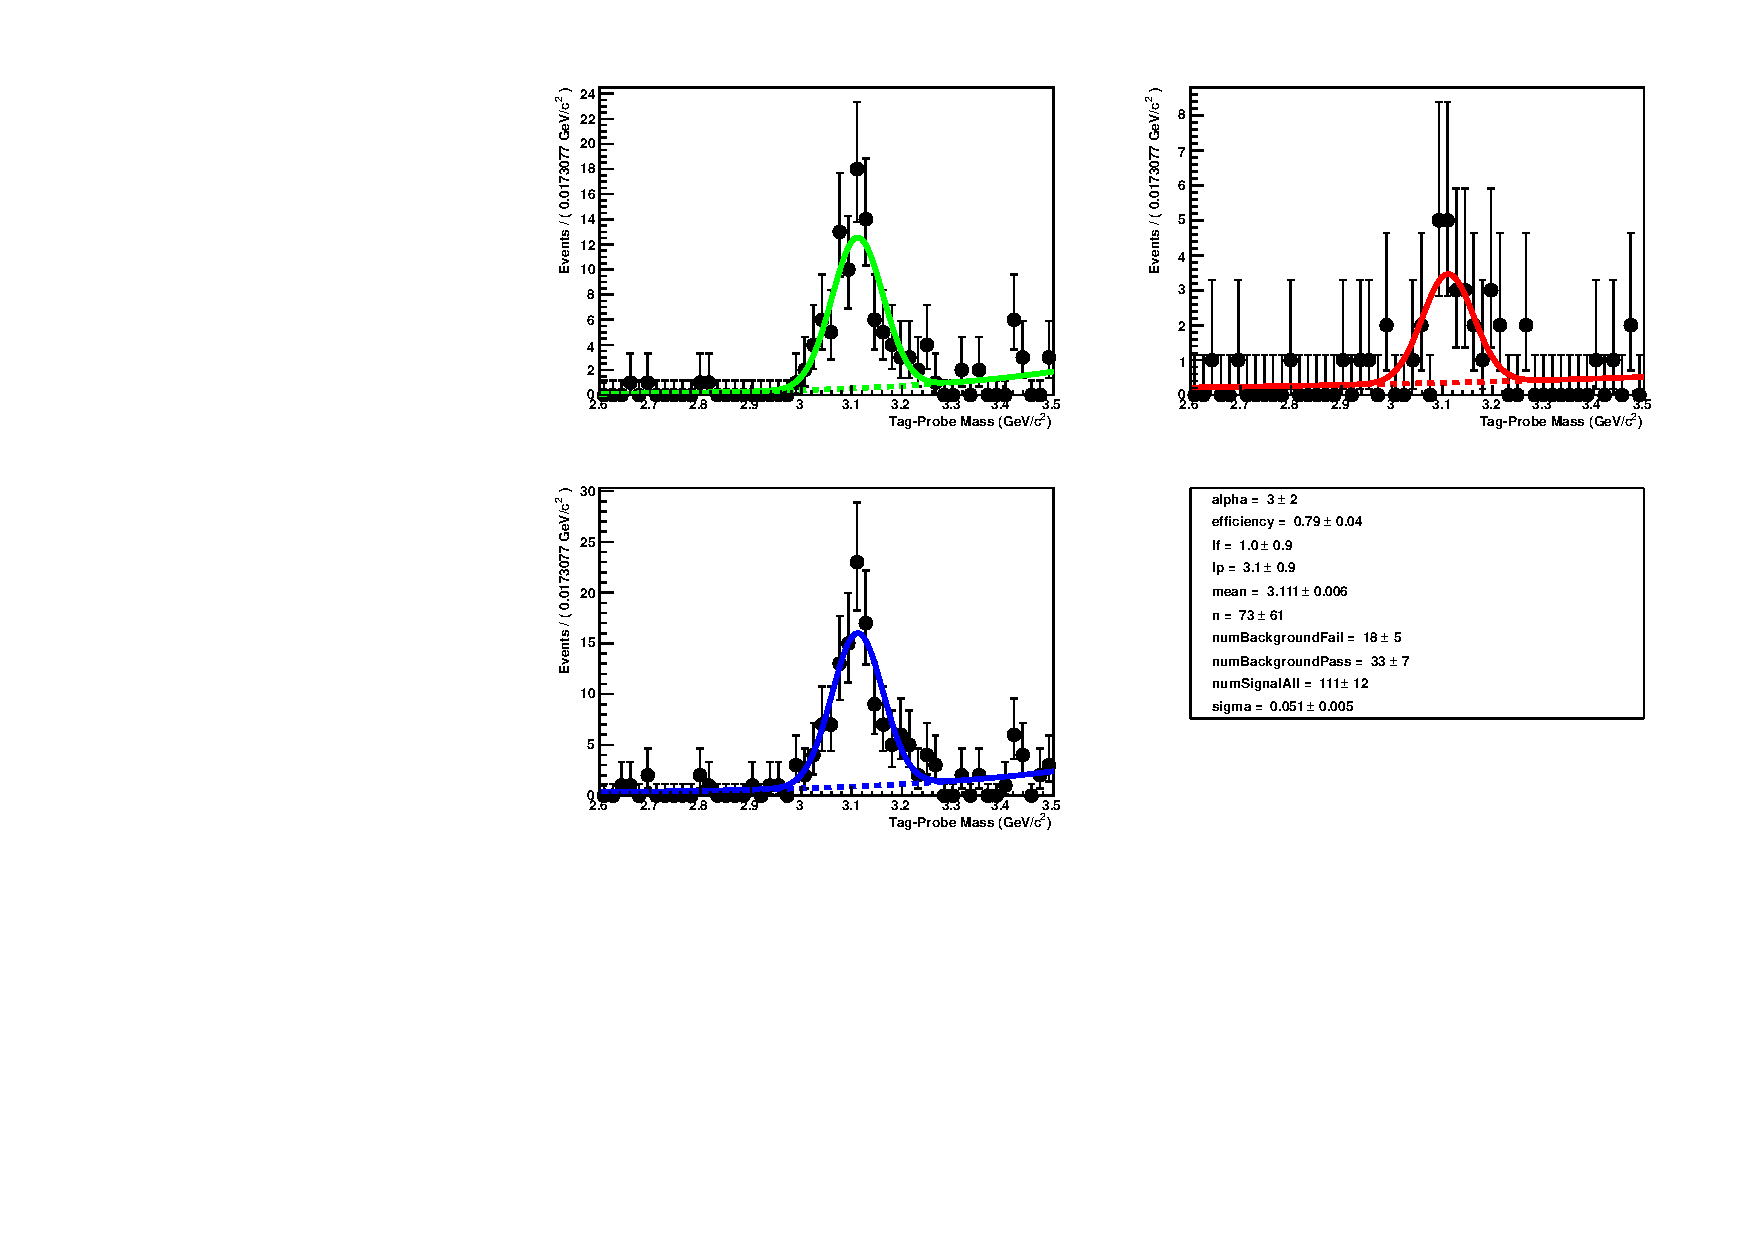
\includegraphics[width=.6\textwidth]{tNp/tnpFits}
        \caption{Fits to tag and probe pairs in the \JPsi{} mass region for
        pairs with a probe 2 < |$\eta$| < 2.2 and 1.55 < \pt{} < 1.8 GeV.}
        \label{fig:tnpFitPlot}
      \end{figure}
      This fit is done for each bin of the probes \pt{} and $\eta$.
      The resulting fit is in Fig.~\ref{fig:tnpTrigMap}.
      \begin{figure}[!Hhbt]
        \centering
        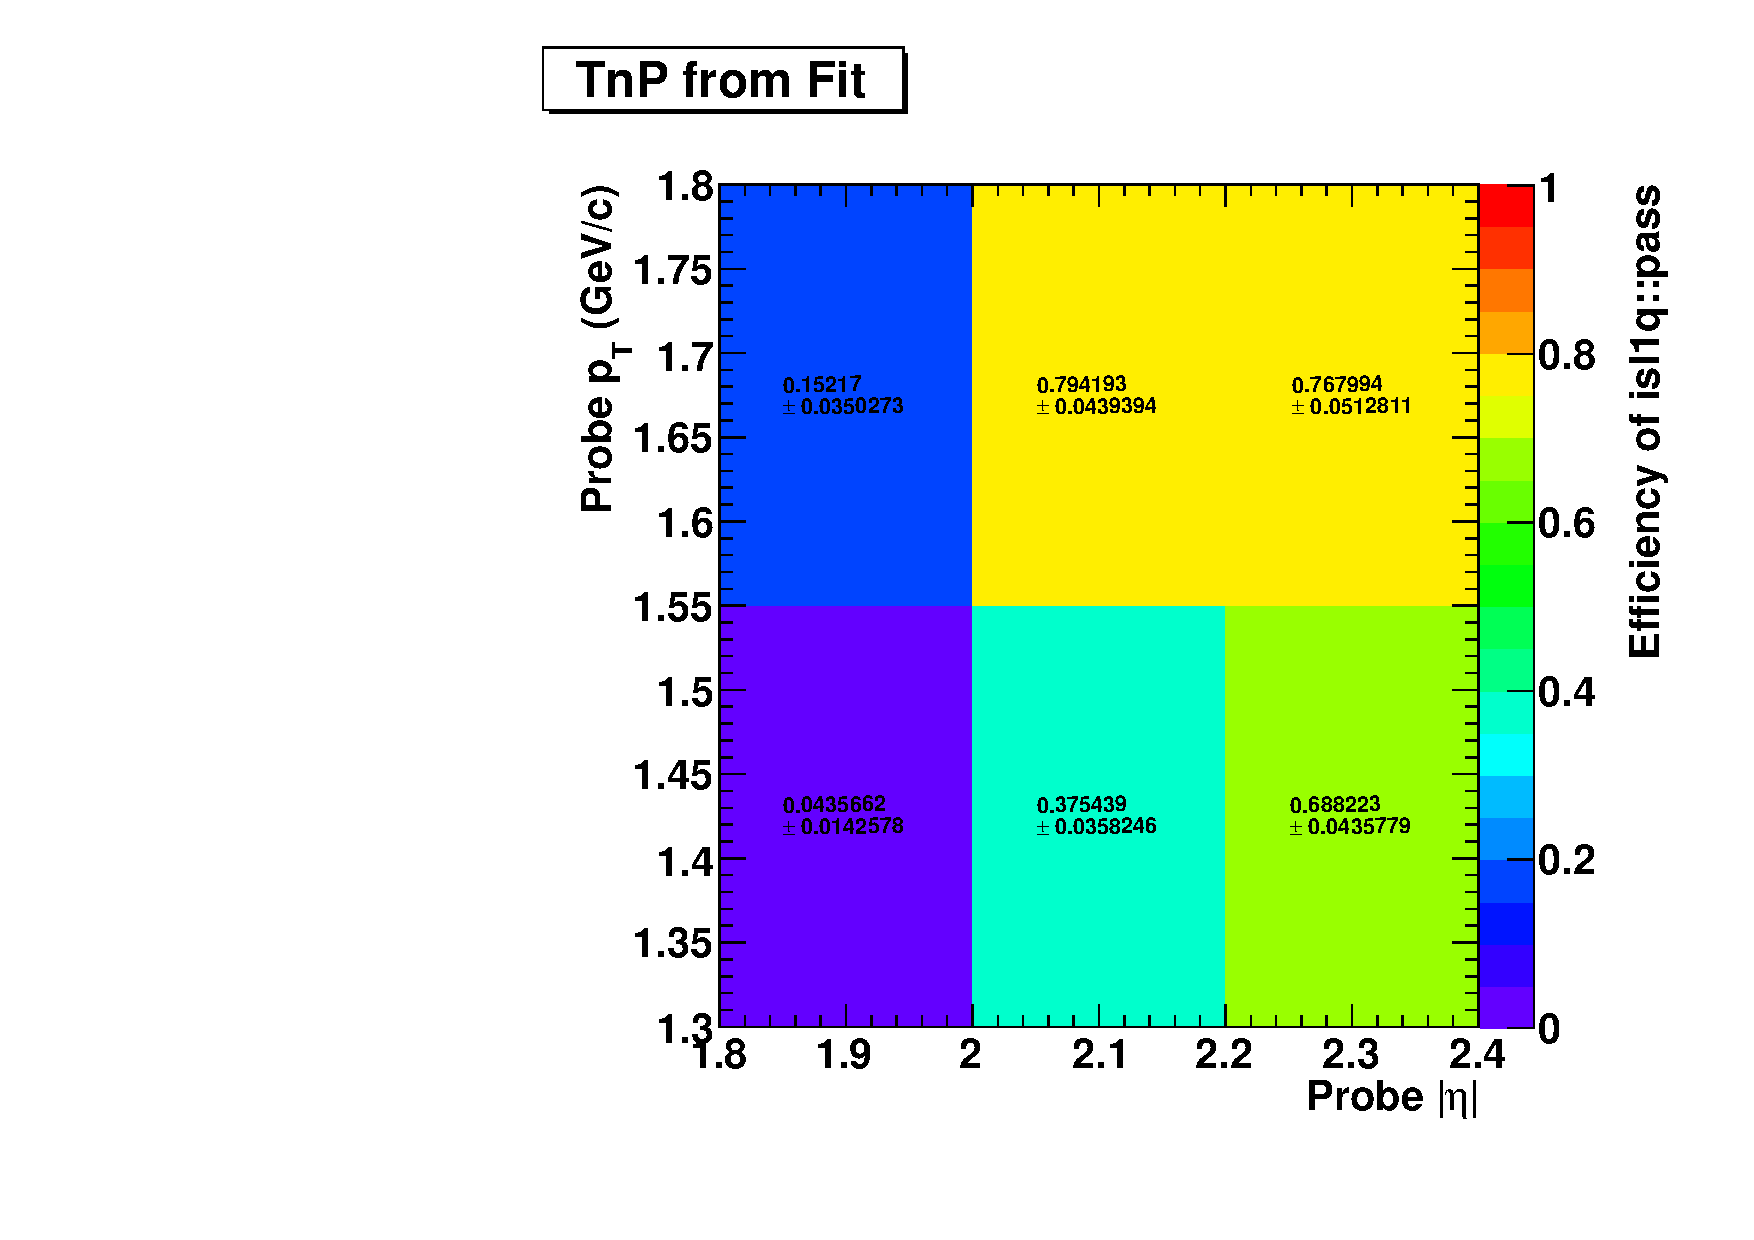
\includegraphics[width=.6\textwidth]{tNp/tnpFromFit}
        \caption{Muon trigger efficiencies in \pt{} and $\eta$ bins from 
          the tag and probe method.}
        \label{fig:tnpTrigMap}
      \end{figure}

      The dimuon trigger efficiency $\varepsilon^{dimuon}_{trigger}$ was measured
        from the single muon efficiencies. 
      The efficiency of each candidate was calculated using the following
        equation:
      \begin{equation}
        \label{eq:dimuTrigEff}
        \varepsilon^{dimuon}_{trigger}=1-(1-\varepsilon_{trigger}^{\mu_{1}})(1-\varepsilon_{trigger}^{\mu_{2}}),
      \end{equation}
      where $\varepsilon_{trigger}^{\mu_{1}}$ is the tag and probe efficiency
        of the first dimuon daughter, and $\varepsilon_{trigger}^{\mu_{2}}$ is
        the efficiency of the second muon daughter. 
      In Eq.~\ref{eq:dimuTrigEff} the probability of at least one daughter
        firing the trigger is calculated by subtracting one from the
        probability that neither daughter fires the trigger,
        thus giving the dimuon trigger efficiency. 

      The average dimuon trigger efficiency for each dimuon (\pt{},$|y|$) bin
        was calculated by averageing the individual dimuon candidates in each
        bin. 
      \begin{figure}[!Hhbt]
        \centering
        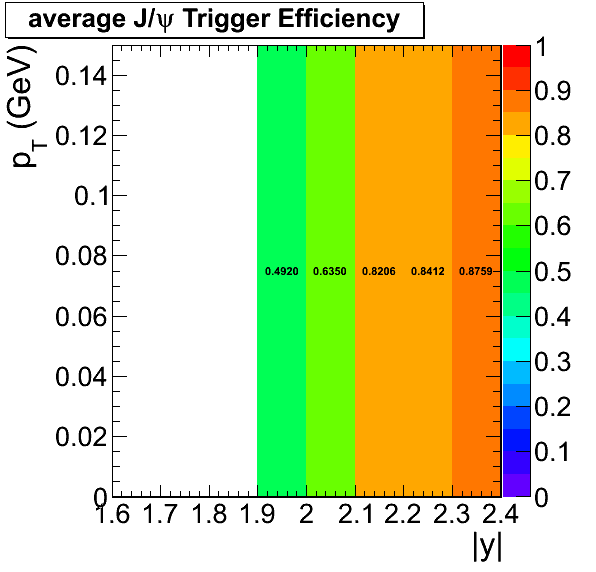
\includegraphics[width=0.6\textwidth]{averageTriggerEff}
        \caption{The trigger efficiency from tag and probe averaged over candidates
          in each (\pt{},$|y|$) bin.}
        \label{fig:avTrigEffCo}
      \end{figure}
      The average trigger efficiency was multiplied by the acceptance from the MC 
        to produce a total factor for both efficiency and acceptance. 
      \begin{figure}[!Hhtb]
        \centering
        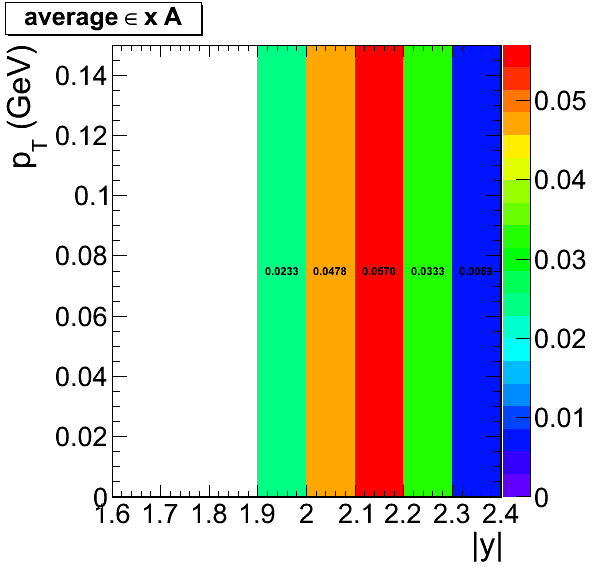
\includegraphics[width=0.6\textwidth]{averageExA}
        \caption{The acceptance times averaged trigger efficiency from tag and 
          probe.}
        \label{fig:avAccEff}
      \end{figure}

      The total combined efficiency and acceptance factor coherent \JPsi{} 
        between 2.0 < |y| 2.2 was found to be around 5\%.
      The roughly 7\% acceptance factor from the MC is the main contributor
        to the total efficiency. 
      Primarily, the interplay of the polarization of the \JPsi{} and
        the material in detector drive down the efficiency by creating an 
        effective momentum threshold for detection (see 
        Section~\ref{sec:mcSim}).
      The reconstruction efficiency of the daughters range between 
        20\%-60\% for muons in the defined detectability range. 
      The trigger efficiency for the detectable muons ranges from 30\%-80\% 
        depending on \pt{}. 
      The typical trigger efficiency for the dimuons ranges from 60\% to 80\%.

    \subsection{ZDC trigger efficiency}
      As discussed in Section~\ref{sec:breakUpDet}, a special trigger was 
        prepared to monitor the ZDC trigger efficiency. 
      This trigger required either a ZDC$^{+}$ or ZDC$^{-}$ trigger, together with at 
        least one pixel track. 
      Events were accepted offline if there was no activity in the BSCs or 
        activity on a single side. 

      This sample suffers from a trigger bias. 
      For example, a sample triggered by ZDC$^{+}$ would always produce a ZDC$^{+}$ 
        trigger efficiency of one. 
      To avoid this, the special trigger sample was divided into two 
        subsamples in the following way. 
      A first sample triggered by the ZDC$^{+}$ input and second one triggered by 
        the ZDC$^{-}$. 
      The ZDC$^{+}$ trigger efficiency is measured from the ZDC$^{-}$ sample, and vice 
        versa.

      The trigger efficiency for reconstructed ZDC energies above the
        single neutron threshold were estimated (see for Sec.~\ref{sec:breakUpDet}).
      The ZDC$^{+}$ efficiency was calculated using the ZDC$^{-}$ triggered 
        sample.
      To estimate the efficiency, the number of events with energy in 
        ZDC$^{+}$ greater than the single neutron threshold, N$_{events}$, 
        were measured.
      From this set of events, the number of events that also fire the 
        ZDC$^{+}$ was measured.
      The ratio between the number of single neutron events that fired the 
        trigger and all single neutron events was taken as the estimate of 
        trigger efficiency. 
      The same procedure was applied for each side of the ZDC.
      The trigger efficiency of the ZDC was found to be 98\% for ZDC$^{-}$
        and 94\% for ZDC$^{+}$.

      \begin{table}
        \centering
        \begin{tabular}{|c|c|c|c|c|}
           ZDC Side & Reco Method & N$_{events}$ & N$_{trig}$ & $\varepsilon_{ZDC}$ \\ \hline
           ZDC$^{+}$ & 1 & 72946  & 71688 & 0.982 $\pm$ 0.005 \\ \hline
           ZDC$^{+}$ & 2 & 73028  & 71706  & 0.9819  $\pm$ 0.005  \\ \hline
           ZDC$^{-}$ & 1 & 76137  & 71786  & 0.9429  $\pm$ 0.005  \\ \hline
           ZDC$^{-}$ & 2 & 76132  & 71859  & 0.9439  $\pm$ 0.005  \\ \hline
        \end{tabular}
        \caption{ZDC trigger efficiencies for ZDC reconstruction method 1 and 
          2}
        \label{tab:zdcEfficiency}
      \end{table}

  \section{\label{sec:sysCheck} Systematic checks}
    
    Table~\ref{tab:sumsyst} shows the systematic errors that were estimated.
    The method used to separate the coherent from the photon-photon process 
     is the most dominant error.
    The ZDC reconstruction method used to estimate the neutron thresholds 
      is the next most dominant, followed by the method used to estimate
      the HF noise threshold. 
    
    \begin{table}[!Hhtb]
      \begin{center}
        \begin{tabular}{|c|c|c|}
          \hline
          systematic & uncertainty in \%  \\ \hline
          Template fit normalized & +9.5\% -12\%    \\ \hline
          ZDC reconstruction  & 2.9\%  \\ \hline
          ZDC trigger efficiency & 2.2\%    \\ \hline
          HF noise threshold & +1.3\% -3.4\%    \\ \hline 
          MC acceptance & 1.1\%    \\ \hline
          \hline \hline
          Total systematic & 8.1\%    \\ \hline
        \end{tabular}
        \caption{Summary of systematic uncertainties}
        \label{tab:sumsyst}
      \end{center}
    \end{table}

    \subsection{HF noise threshold}
      The way in which the HF noise distribution is measured effects the event 
        selection and therefore the final candidate yeild.
      This cut plays a significant role in rejecting hadronic events.
      In Table~\ref{tab:evSelCutNumbers} the importance of cutting on HF noise
        is evident. 
      The HF noise cut rejects a little less than 1/5 of the remaining events. 
      The systematic uncertainties on the HF noise requirement is important for
        this reason.
      The result must not depend significantly on the method used to apply the
        cut on the noise because of the large reduction of events that result
        from it. 
      
      Four different approaches were employed to estimate the systematic effect
        arising from picking a particular method for setting the HF noise
        threshold. 
      By looking at the variation of the number of events that remain after 
        applying the thresholds derived from these four methods, the systematic
        uncertainty for the HF noise cut was estimated.
      The four methods are derive from combinations of two variations. 
      The type of object was varied from a low-level detector object called a 
        RecHit to a higher level physics object called a CaloTower. 
      The RecHit is the energy deposited in a single calorimeter detector 
        element, where as the CaloTower is a collection of RecHits with 
        varrious threholds, which represent a full energy deposit that would 
        come from a particle or a collection of particles from a jet passing 
        through the detector. 
      The second variation is on the separation of the two sides.
      In one case the threshold is derived for the two sides combined.
      In another case the thresholds are calculated separately for the two 
        sides of HF.
      By combining these two variations, a total of four estimates of the 
        effect of the HF noise cut were made.
      Table~\ref{tab:hfNoiseThreshAsym} below shows the thresholds that are 
        measured for each of the four methods.
      The resulting yields from the four different methods are displayed in 
        Table~\ref{tab:hfCutYieldEffects}.

      \begin{table}[!Hhbt]
        \centering
        \begin{tabular}{|c|c|c|c|}
          \hline
          Object type & HF (GeV) & HF$^{-}$ (GeV) & HF$^{+}$ (GeV) \\ \hline
          RecHits & 3.85 & 3.25 & 3.45 \\ \hline
          CaloTowers & 4.25 & 3.25 & 3.75 \\ \hline
        \end{tabular}
        \caption{HF noise theresholds for various noise measurement methods.}
        \label{tab:hfNoiseThreshAsym}
      \end{table}

      \begin{table}[!Hhbt]
        \centering
        \begin{tabular}{|c|c|c|}
          \hline
          Object type & Combinded HF threshold & Two-sided thresholds \\ \hline
          RecHits & 298 & 290 \\ \hline
          CaloTowers & 302 & 288 \\ \hline
        \end{tabular}
        \caption{Candidate yields below 1.05 GeV \pt{} for various HF noise
          cuts.}
        \label{tab:hfCutYieldEffects}
      \end{table}

      The threshold was adjusted to estimate the effect of tightening the
        requirement on the zero bias data.
      By successively lowering the percentage of the zero bias sample
        that was included, the HF noise cut was made more restrictive including
        first 98\%, than 97\% of all zero bias events. 
      This was done for both object types, RecHits and CaloTowers.
      This allows for an estimate of the systematic uncertainty on selecting 
        a 99\% cut.
      Table~\ref{tab:hfAdjustedThresholds} shows the effect on the thresholds
        themselves for both RecHits and CaloToweres, whereas 
        Table~\ref{tab:hfAdjThreshYields} shows the effect on the candidate 
        yields.

      \begin{table}[!Hhbt]
        \begin{center}
          \caption{Values of the energy cuts for the HF calorimeter for RecHit and CaloTower in GeV.}
          \label{tab:hfAdjustedThresholds}
          \begin{tabular}{|c|c|c|} \hline
            \% &  $E_{RecHit}$ GeV & $E_{CaloTower}$ GeV\\ 
            \hline
            99 & 3.85& 4.25 \\ \hline
            98 & 3.25& 3.75 \\ \hline
            97 & 2.95& 3.25 \\  \hline
           \end{tabular}
         \end{center}
      \end{table}

      \begin{table}[!Hhbt]
        \begin{center}
          \caption{Number of dimuon candidates with  p$_{T} <$1.05 when changing HF calorimeter cuts for RecHit and CaloTower.}
          \label{tab:hfAdjThreshYields}
          \begin{tabular}{|c|c|c|} \hline
            \% &  RecHit cut & CaloTower cut\\ \hline
            99 &   298 & 302 \\ \hline
            98 &  287  & 294 \\ \hline
            97 & 284 & 280 \\ \hline
          \end{tabular}
        \end{center}
      \end{table}

      The systematic uncertainty in the HF noise threshold measurement was 
        calculated taking the difference from the 99\% combined RecHit method
        with the upper and lower extrema. 
      The systematic uncertainty from this method is calculated to be +1.3\% 
        -3.4\%.


    \subsection{Template fit normalization}
      \begin{figure}[!Hhtb]
        \centering
        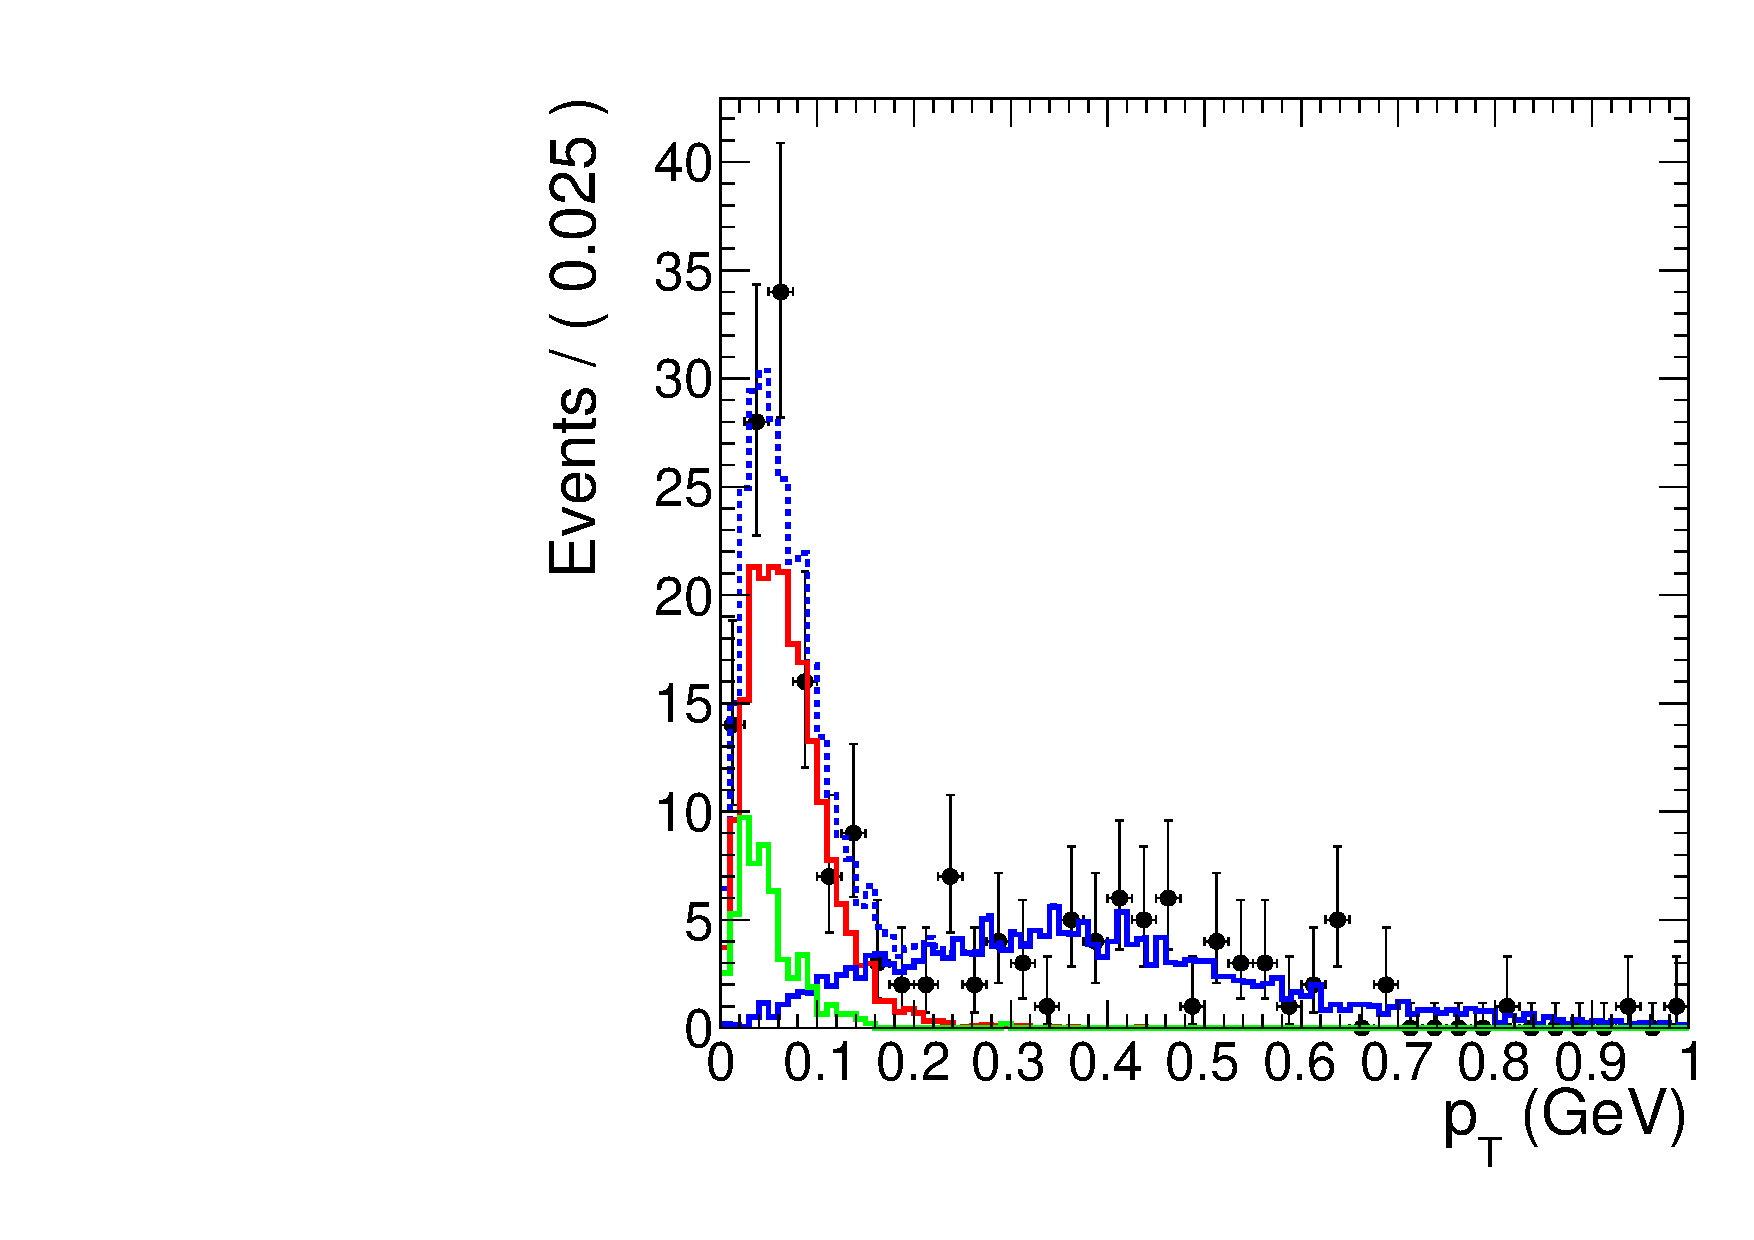
\includegraphics[width=.6\textwidth]{ptOnly}
        \caption{Coherent, incoherent, and photon-photon process \pt{} template fit to data.}
        \label{fig:ptTempFit}
      \end{figure}
     
      The \pt{} template fit depends on the functions chosen for the fit
        to the mass distribution.
      As described in Section~\ref{sec:sigEx}, the similarity of the of the 
        \pt{} distribution for the coherent and photon-photon process make
        the contributions from the two process difficult to separate from the 
        \pt{} distribution alone.
      The mass distribution was used to distinguish between these two processes.
      In turn, the \pt{} becomes dependent on the mass fit. 

      The systematic uncertainty due to the choose of functions used to fit
        the mass distribution was estimated by varying the signal and 
        background functions.
      The contribution to the background from the mass fit was used to fix the
        contribution from the photon-photon process in the \pt{} template
        fit.
      Two functions were used to describe the signal, a Gaussian, and a Crystal
        ball function. 
      The background was fit to a linear function, a 2nd order polynomial, and
        a 2nd order Cheby-Chev polynomial. 
      The resulting variation on the coherent contribution was used to as an
        estimate of this systematic effect. 

      \begin{figure}[!Hhbt]
        \centering
        $ \begin{array}{ccc}
          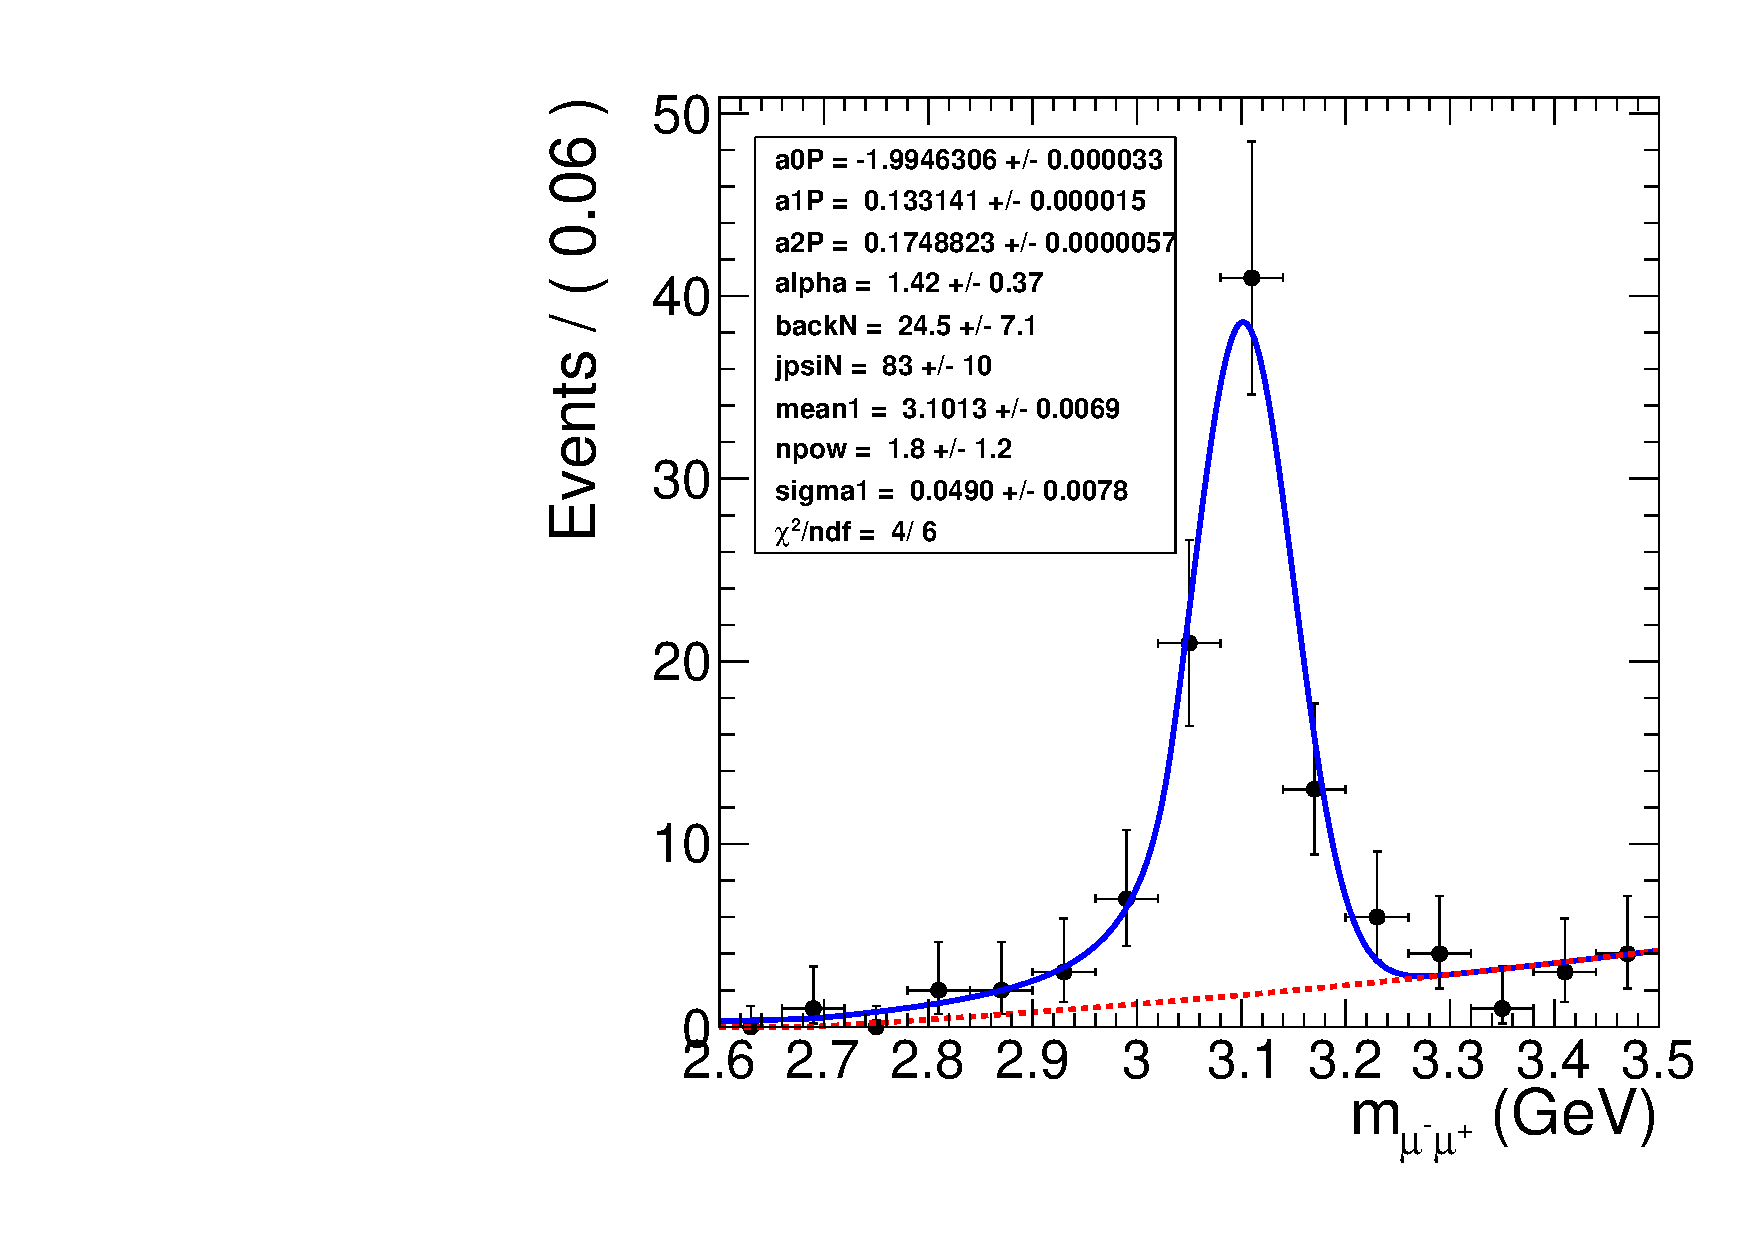
\includegraphics[width=.3\textwidth]{cbPolyBkgEst} &
          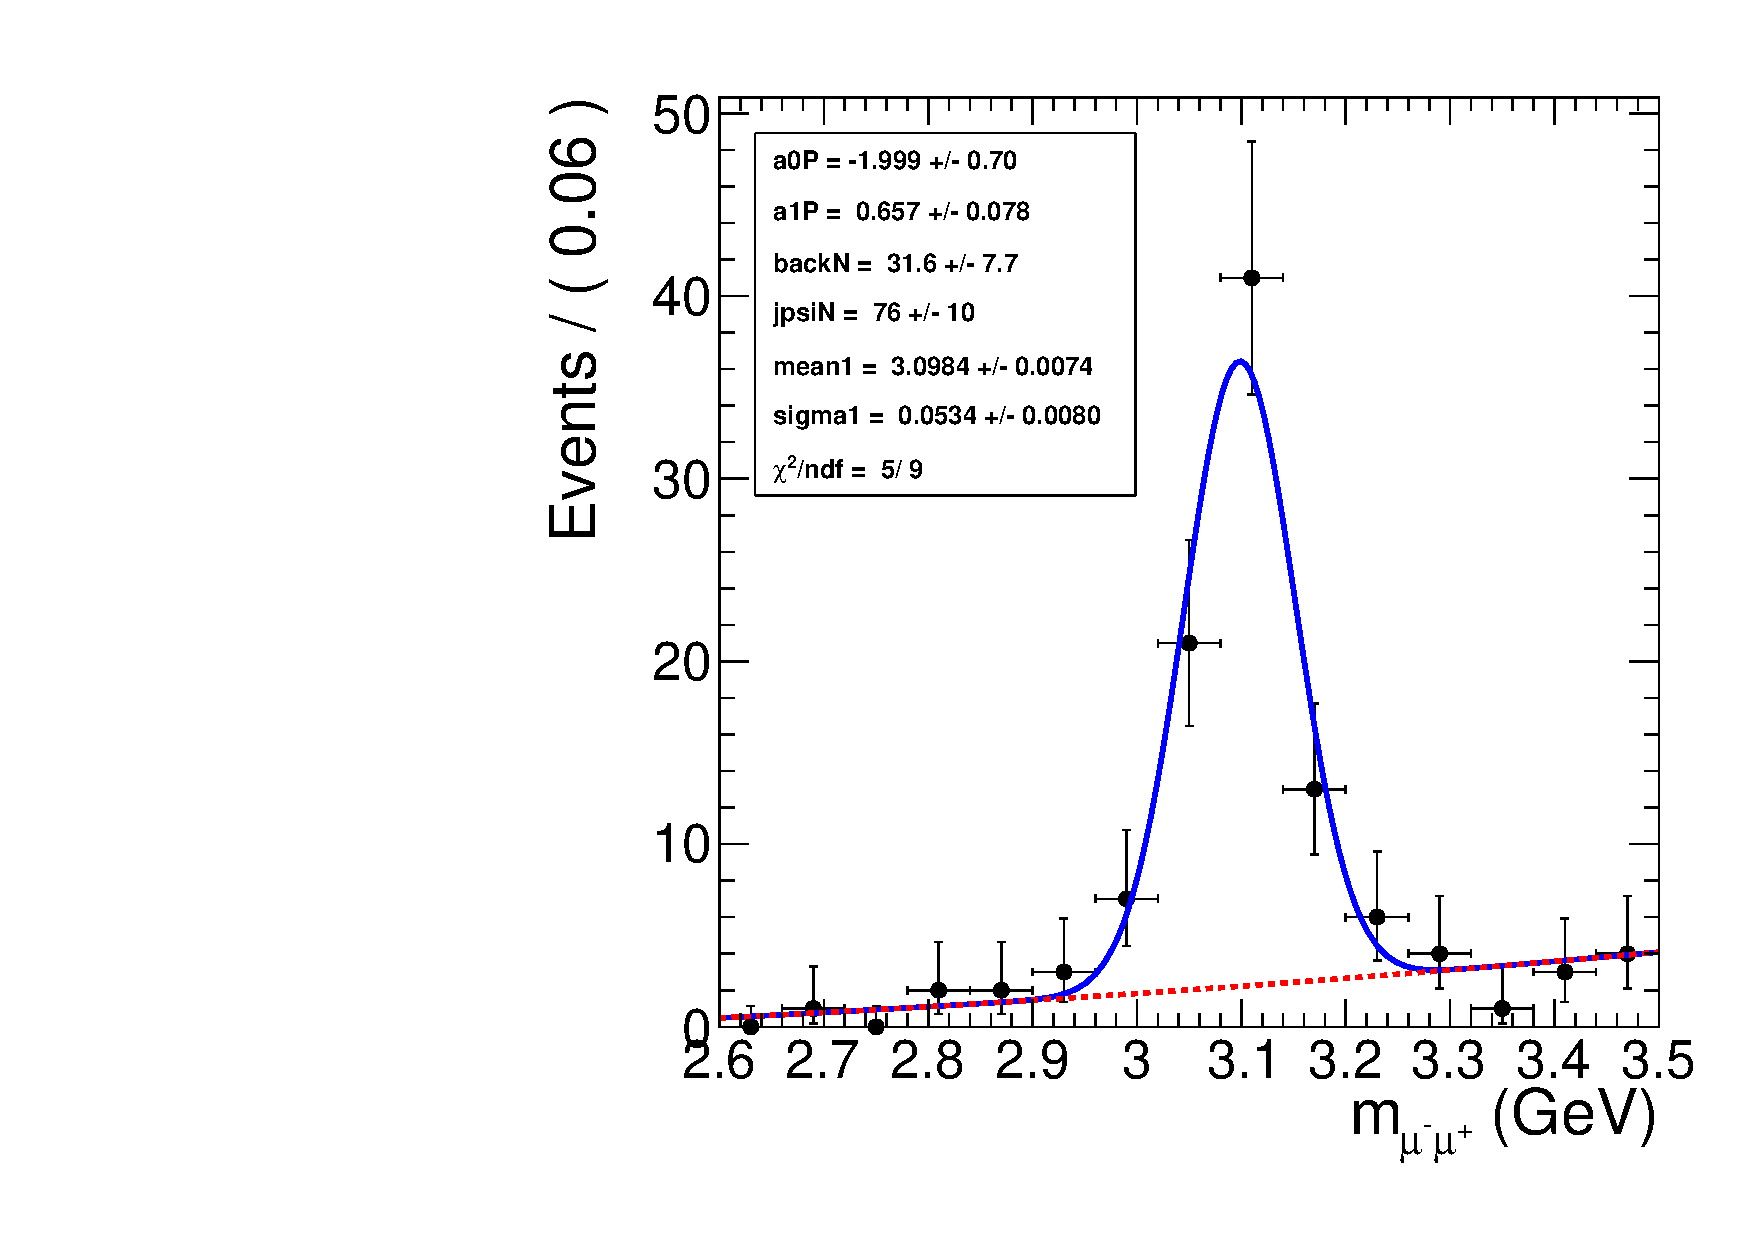
\includegraphics[width=.3\textwidth]{gausLinBkgEst} &
          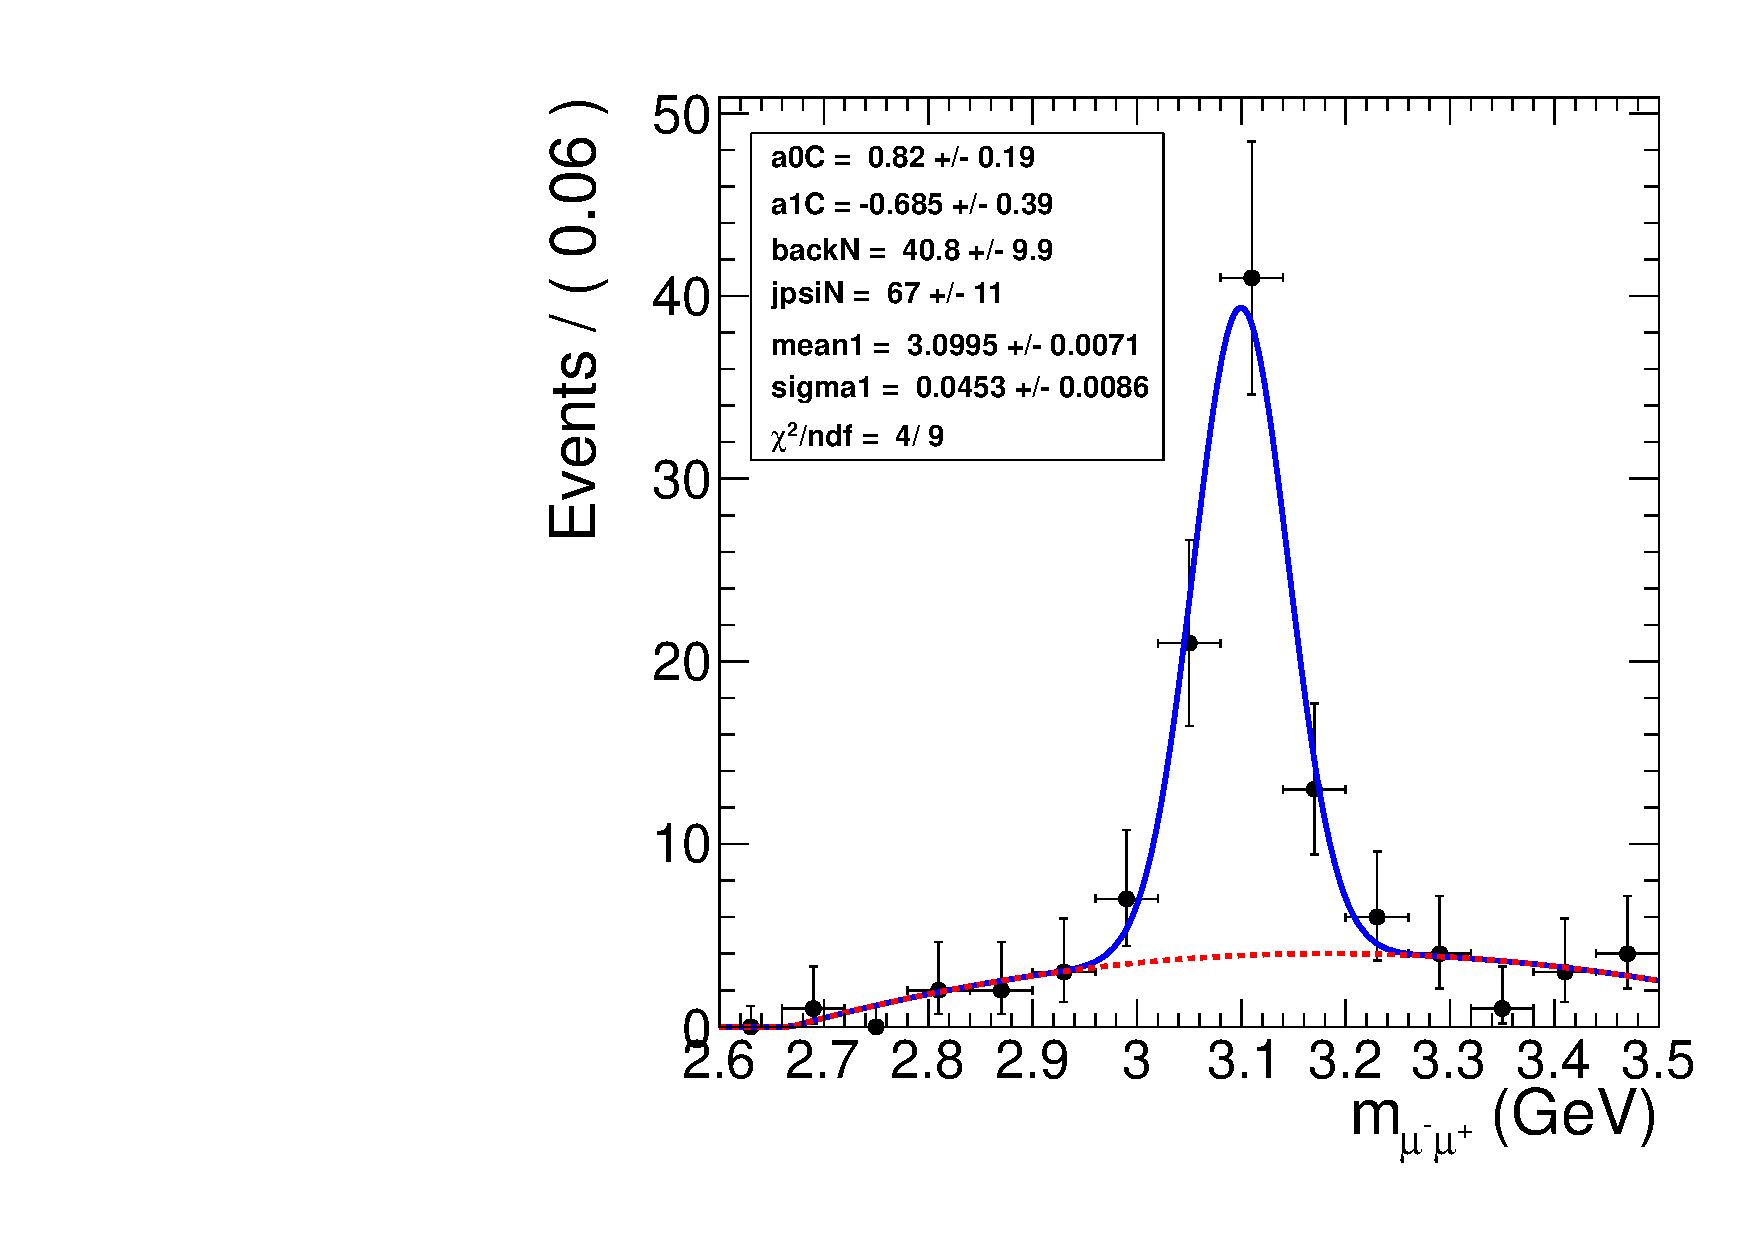
\includegraphics[width=.3\textwidth]{gausCCBkgEst} \\
          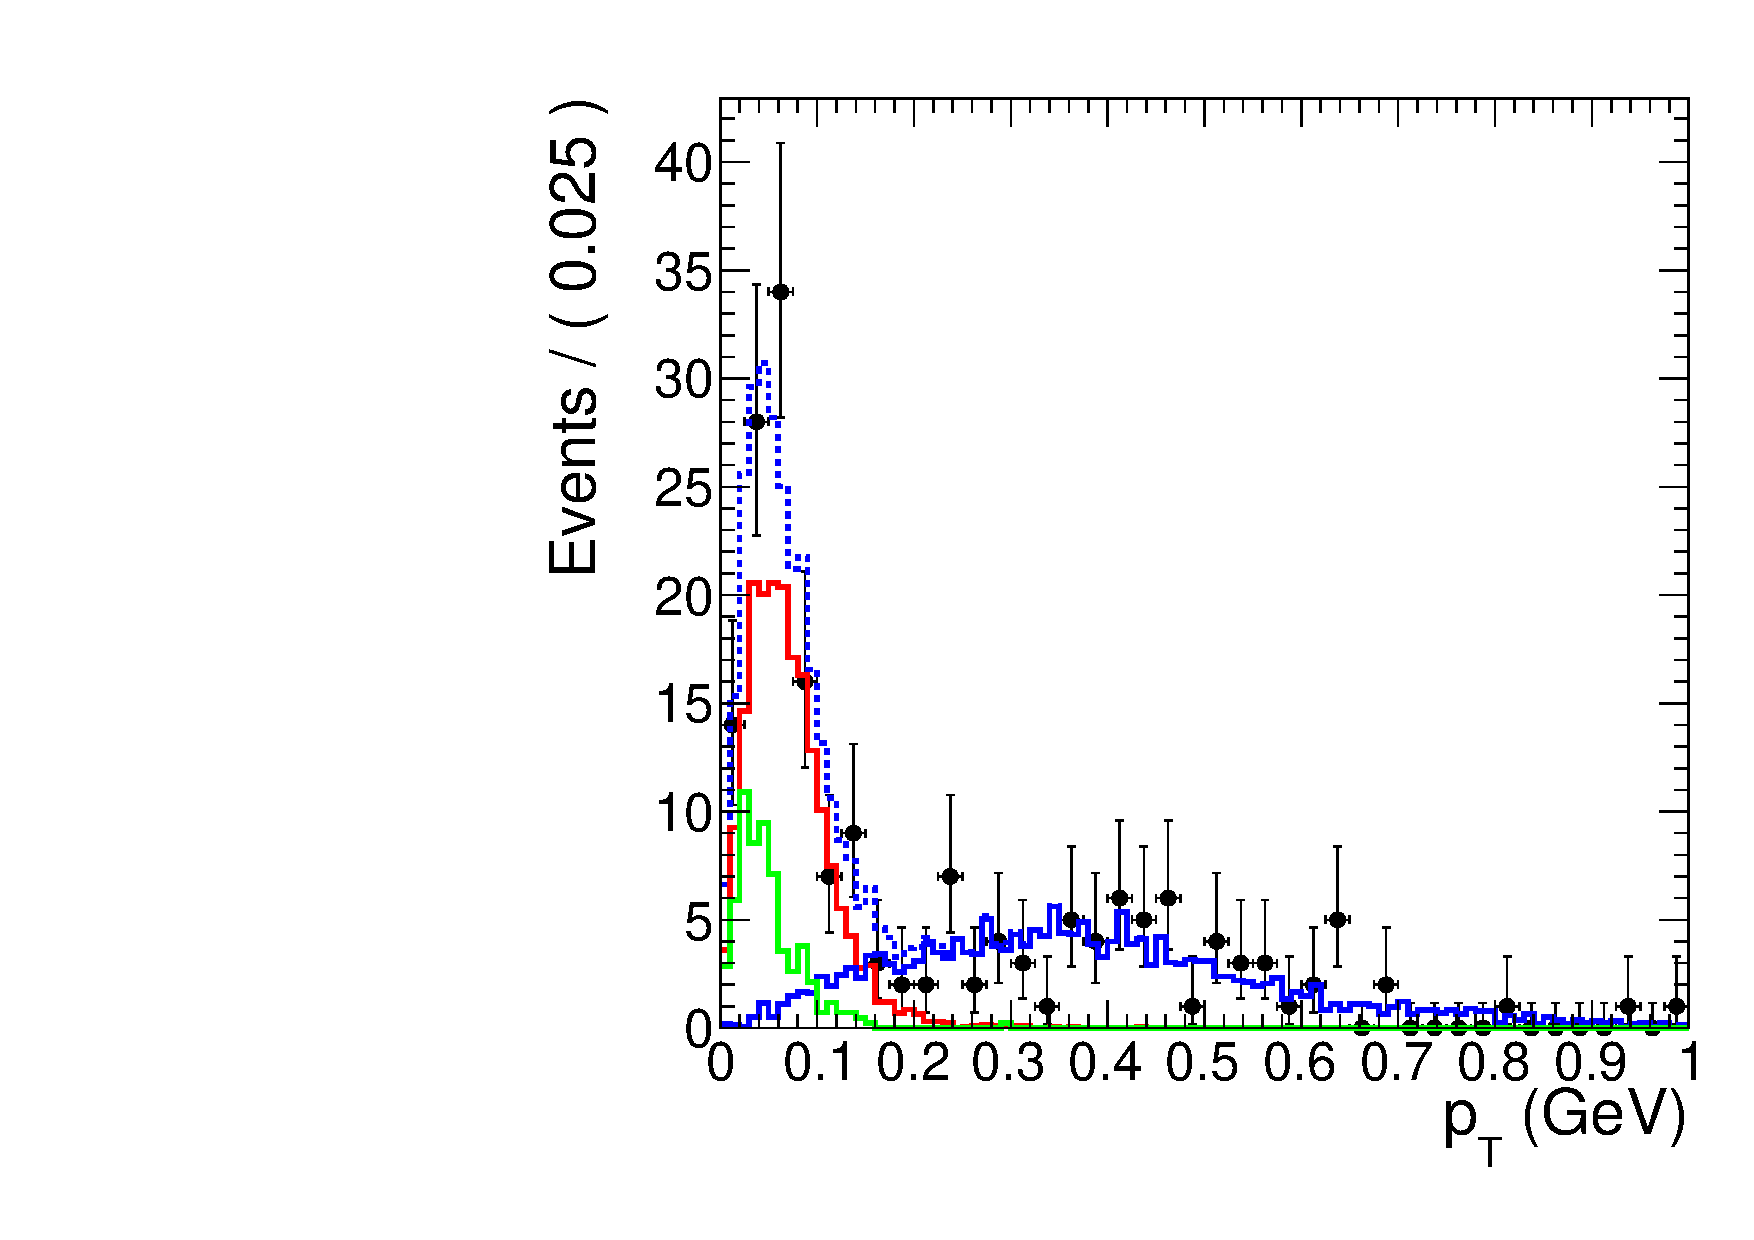
\includegraphics[width=.3\textwidth]{cbPoly} &
          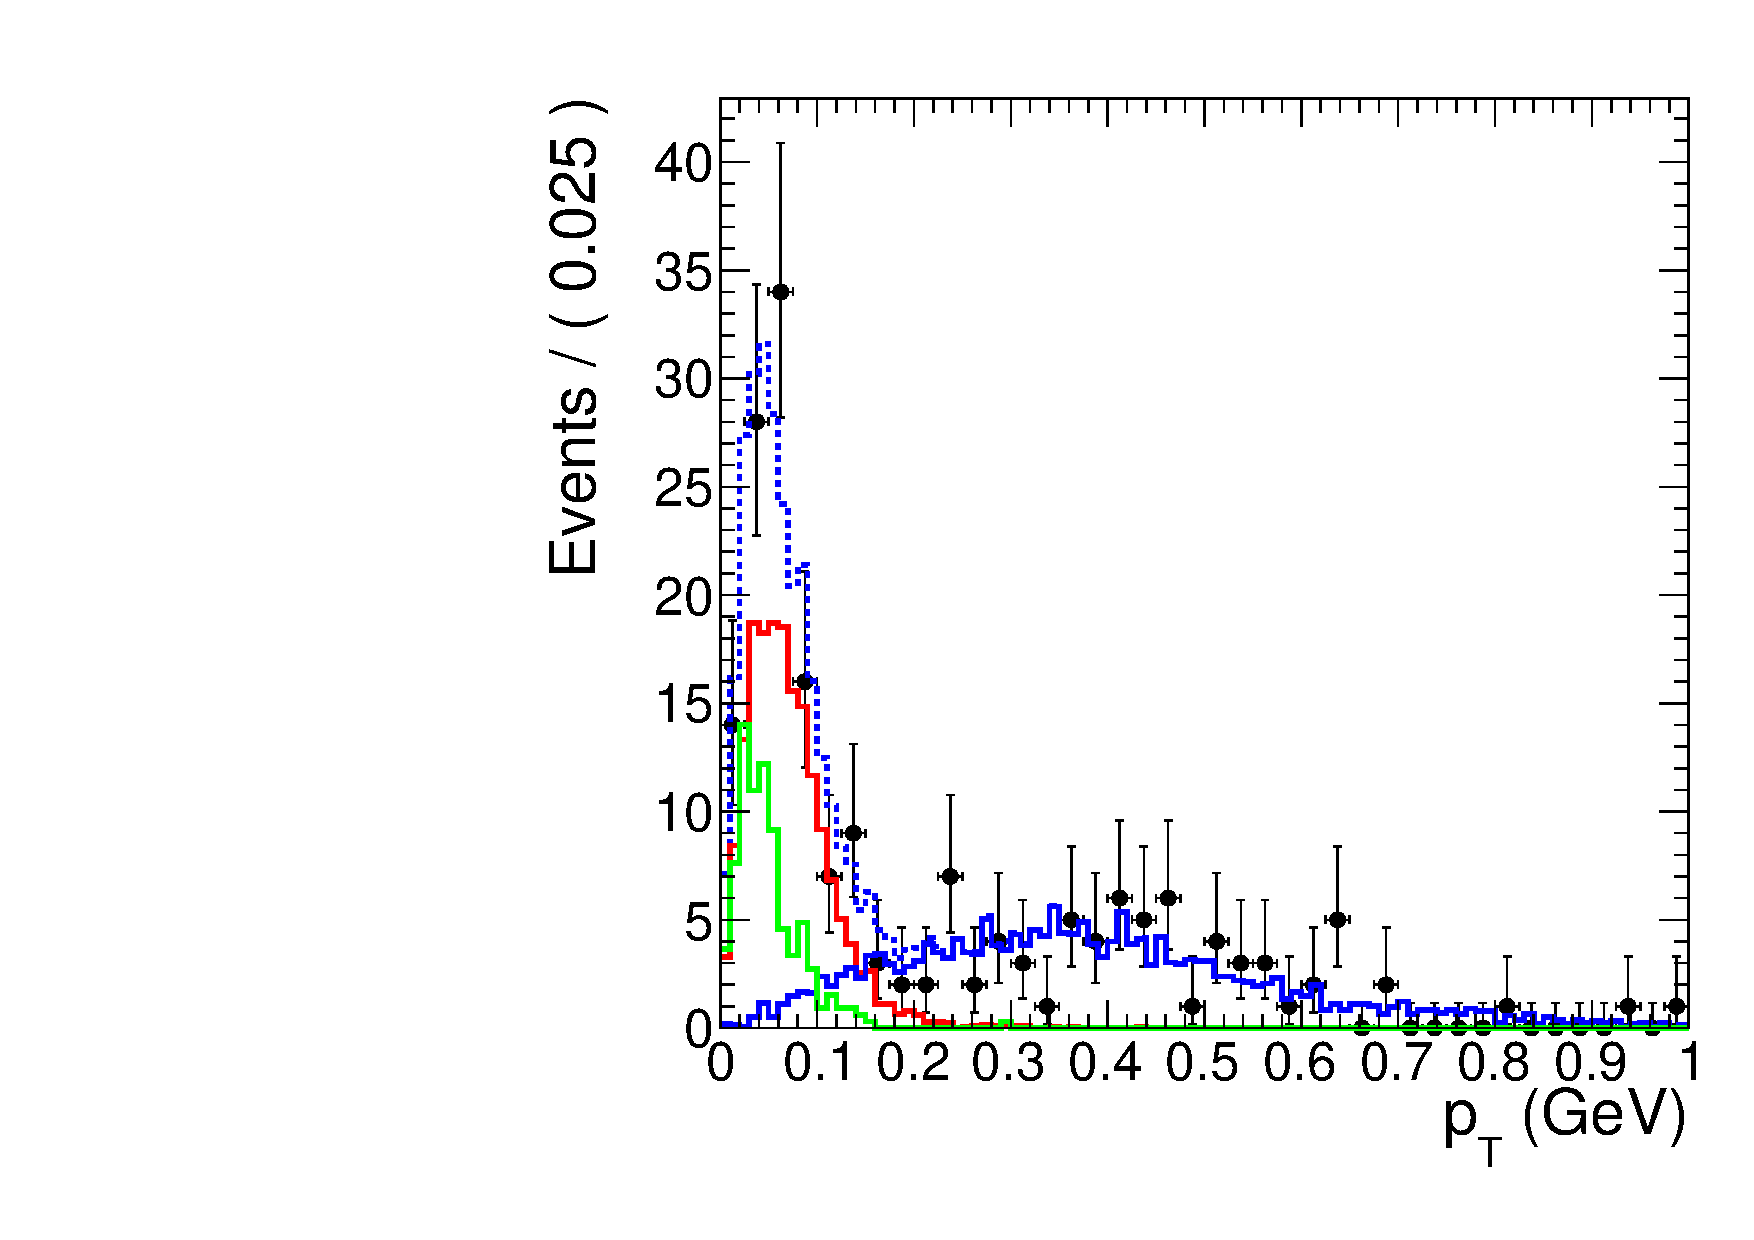
\includegraphics[width=.3\textwidth]{gausLin} &
          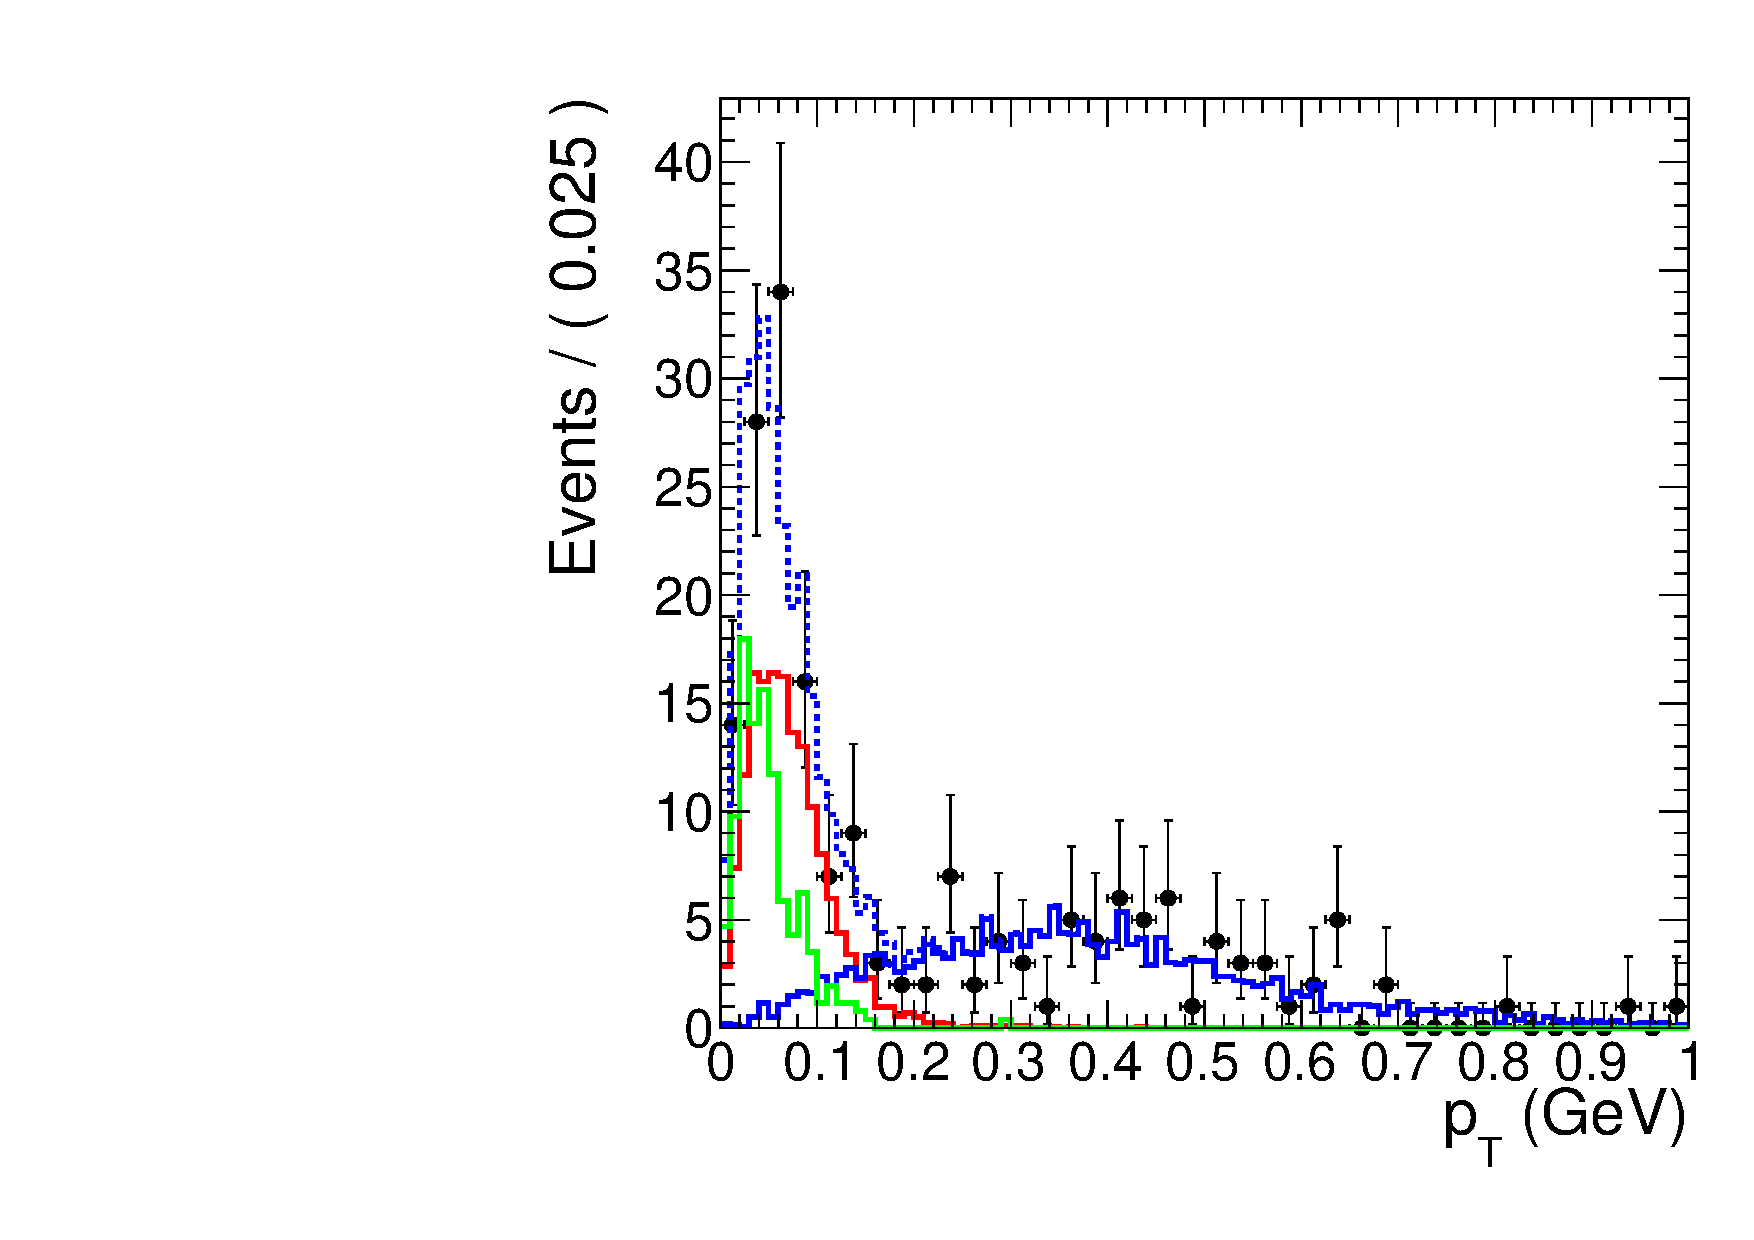
\includegraphics[width=.3\textwidth]{gausCC}
        \end{array} $
        \caption{Various mass distribution fits and the corresponding \pt{}
          template fit.}
        \label{fig:massPtFitsForSyst}
      \end{figure}

      Moving from left to right in Fig~\ref{fig:massPtFitsForSyst}, the 
        contribution from the photon process increases.
      The $\chi^{2}$ pre degree of freedom is similar between the three 
        fits indicating a similar goodness of fit.
      On this basis, neither fit is preferred. 
      The left most fit uses a Crystal Ball function to account for the 
        radiative decay of the final state daughters of the \JPsi{}.
      The low mass exponential portion however picks up background events 
        and overestimates the \JPsi{} contribution. 
      The right most plot fits the background to a 2nd order Cheby-Chev 
        polynomial.
      Because the Cheby-Chev peaks just below the \JPsi{} peak, this fit 
        overestimates the background and in turn underestimates the signal 
        contribution.
      The Gaussian fit with a linear background however does a reasonable job
        of fitting both the background and the signal. 

      From these three fits an upper and lower bound of the systematics due
        the choice of fit functions was estimated. 
      The difference between the Gaussian-Linear fit and the 
        Crystal Ball-polynomial fit was taken as an upper bound. 
      The difference between the Gaussian-Linear fit and the 
          Gaussian-Cheby-Chev fit was taken as a lower bound. 
      The overall systematic uncertainty due to the choose of mass fit 
        functions is found to be +9.5\% -12\%.

    \subsection{Mass fit}
      
      \begin{figure}[!Hhtb]
        \centering
        $ \begin{array}{cc}
          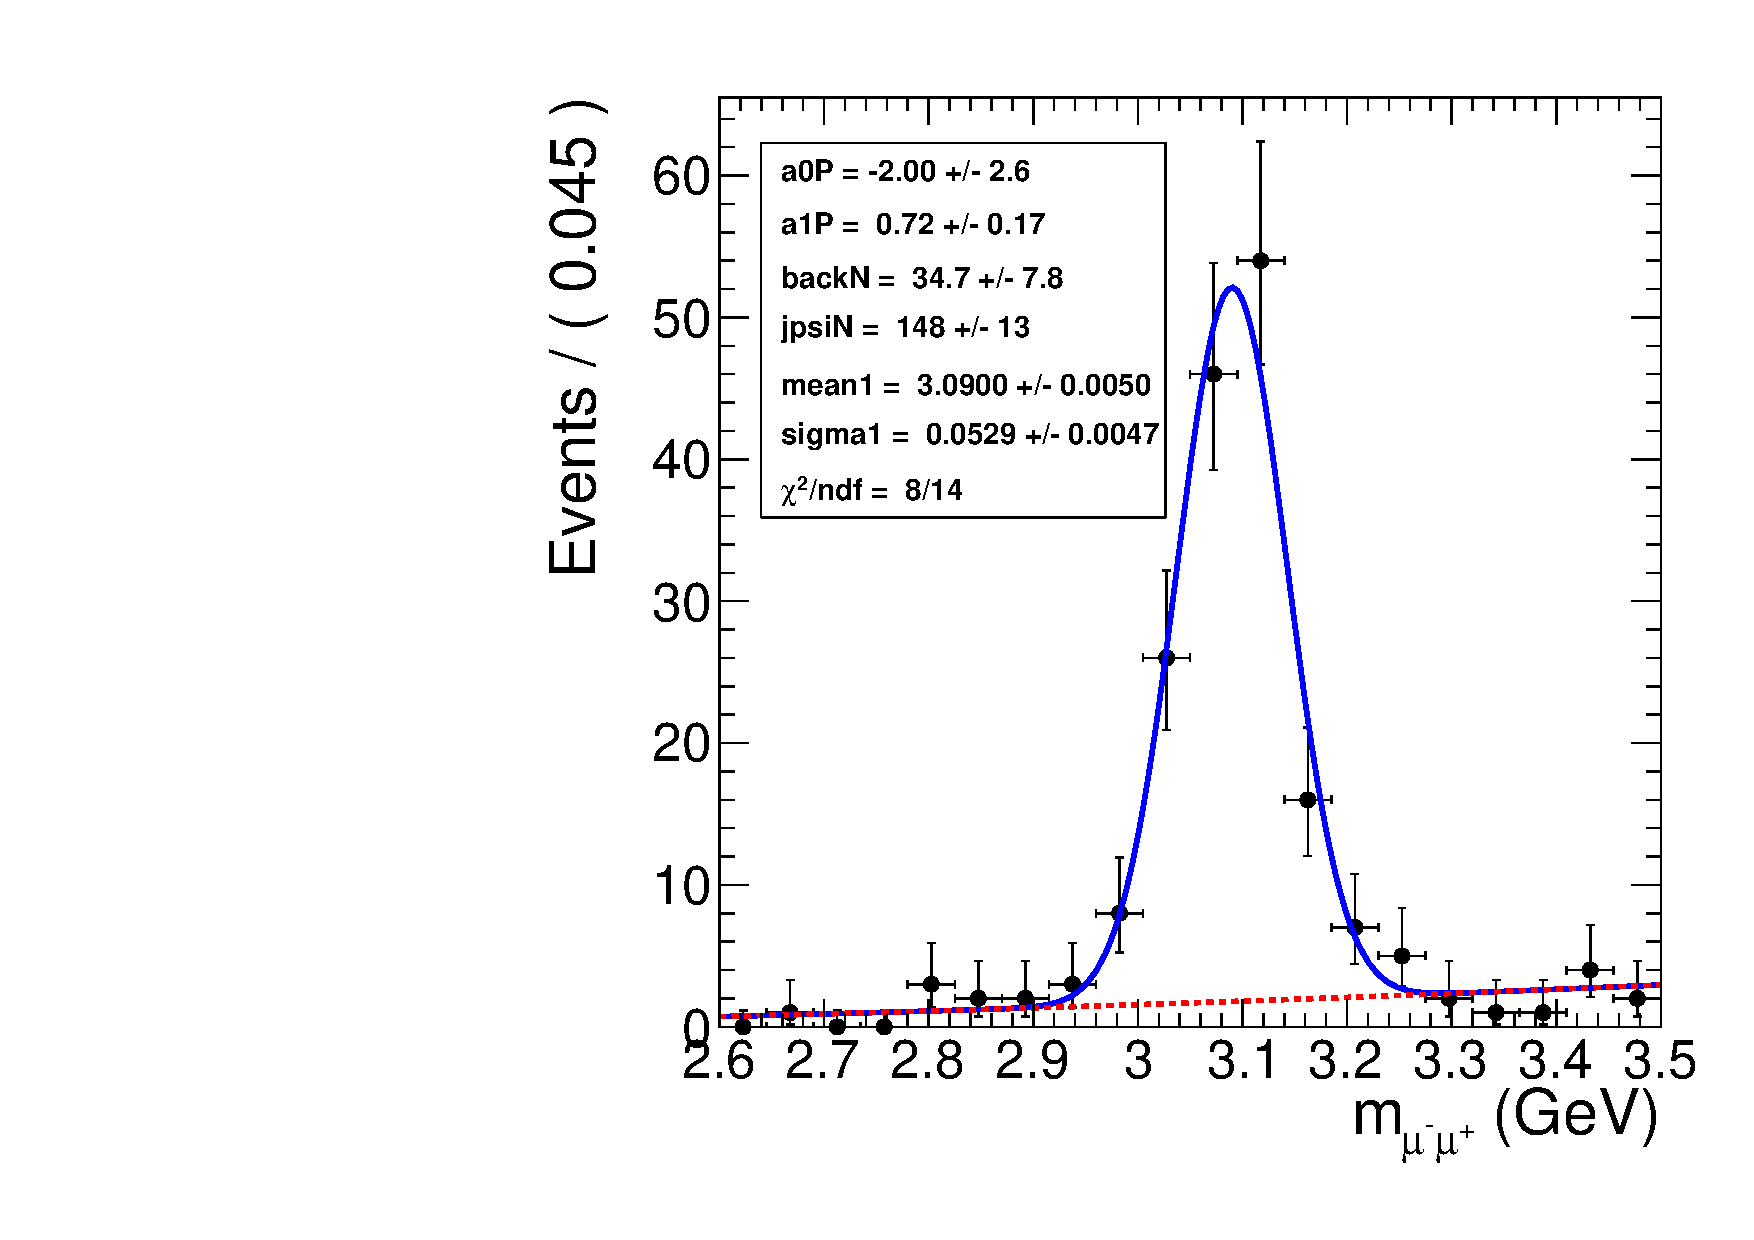
\includegraphics[width=.45\textwidth]{massFitSimple} &
          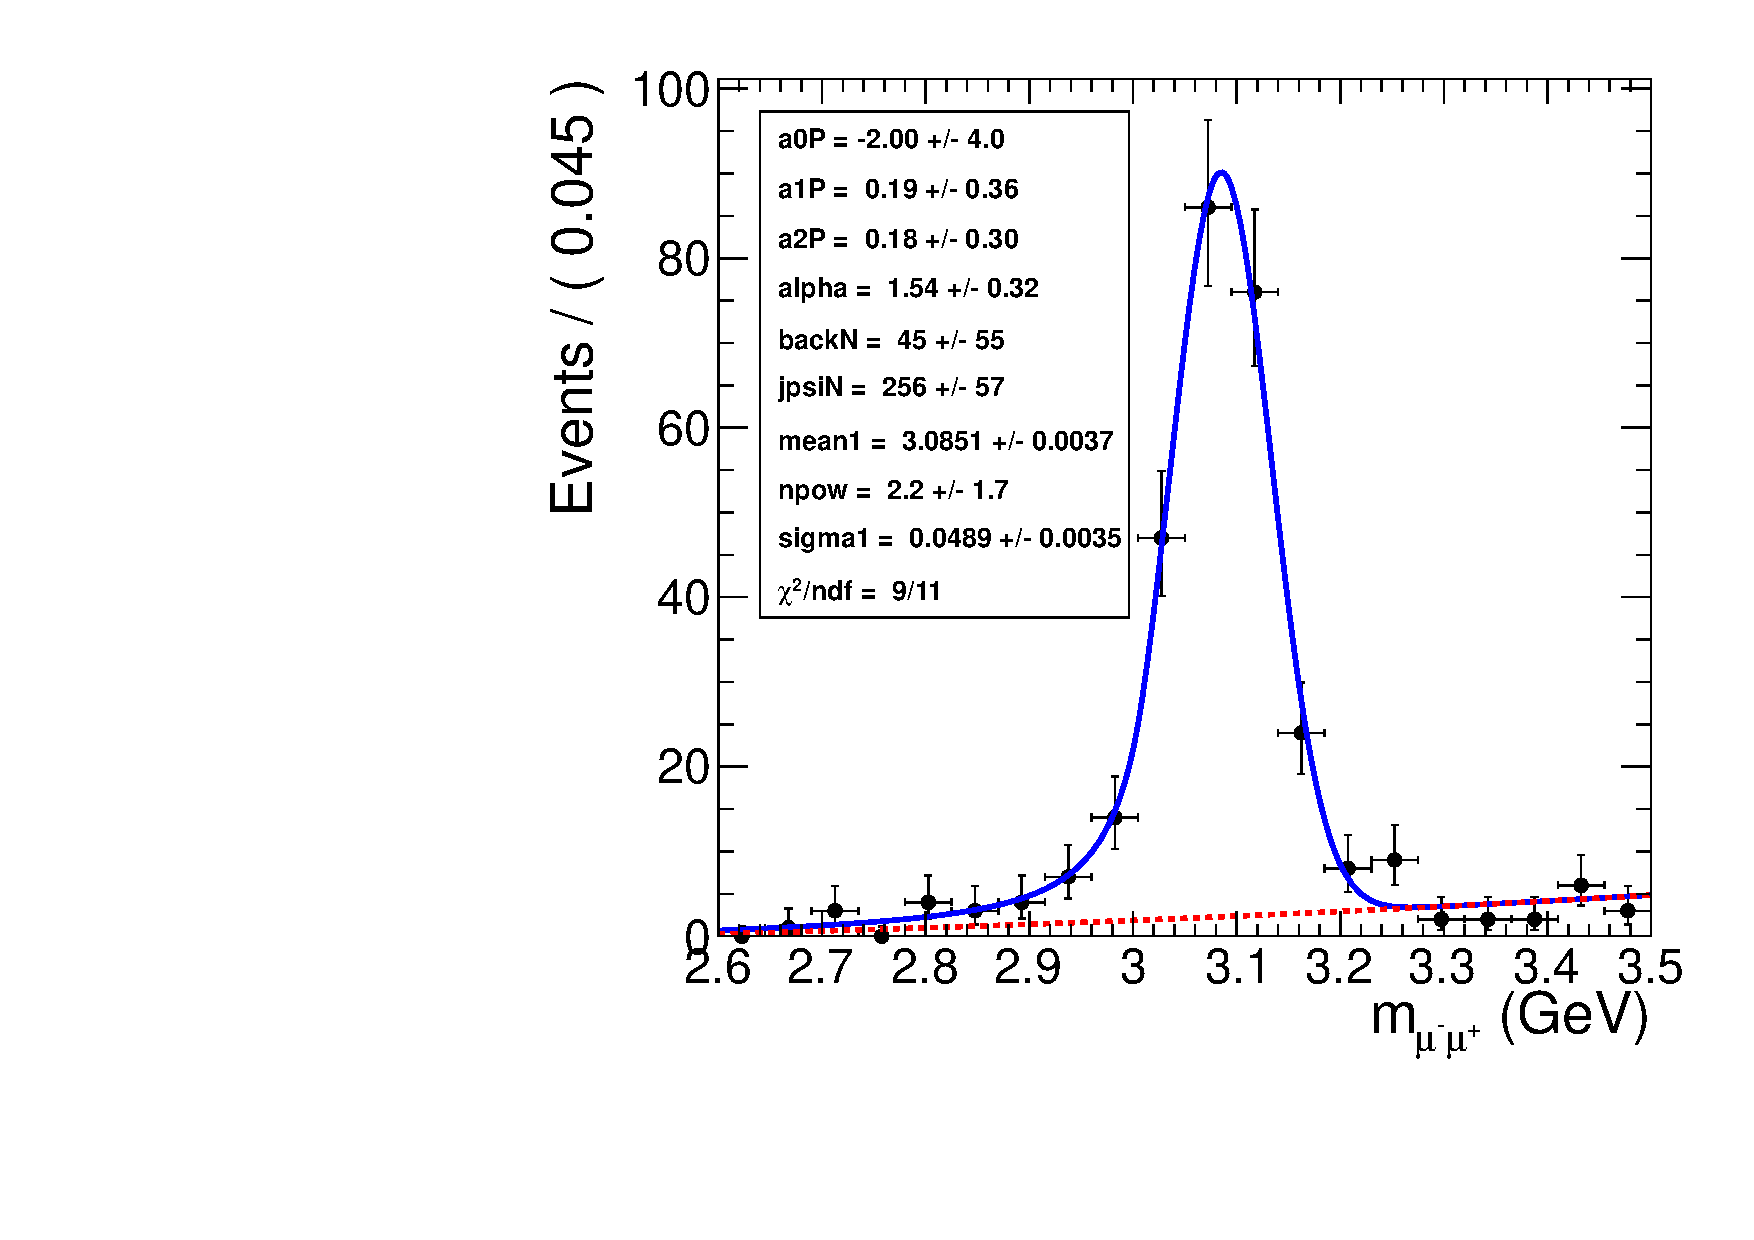
\includegraphics[width=.45\textwidth]{massFitCBPoly2}
        \end{array} $
        \caption{Mass fit to \JPsi{} using Gaussian (Left) and Crystal Ball (Right) for the 
          signal and a polynomial for the background}
        \label{fig:massFitSys}
      \end{figure}
      Fig.~\ref{fig:massFitSys} demonstrates the small dependence the raw 
        \JPsi{} yield has on the fitting function. 
      Both fit functions agree well, with reduced $\chi^{2}$ values below one.
      The Crystal ball fit give an upper estimate for the \JPsi{} yield.
      The Gaussian fit gives an lower estimate. 
      The main difference comes from the lower mass tails.
      In the Crystal ball fit the lower tail is considered to be signal due to 
        shifting of the mass spectrum to lower mass due to radiation from the 
        final state muons. 
      In the Gaussian fit the lower mass tail is considered to be background and 
        the signal is sharper.

      As check on the simultaneous \pt{} and mass fit, the mass fit is done
        using mass templates from STARlight.
      \begin{figure}[!Hhbt]
        \centering
        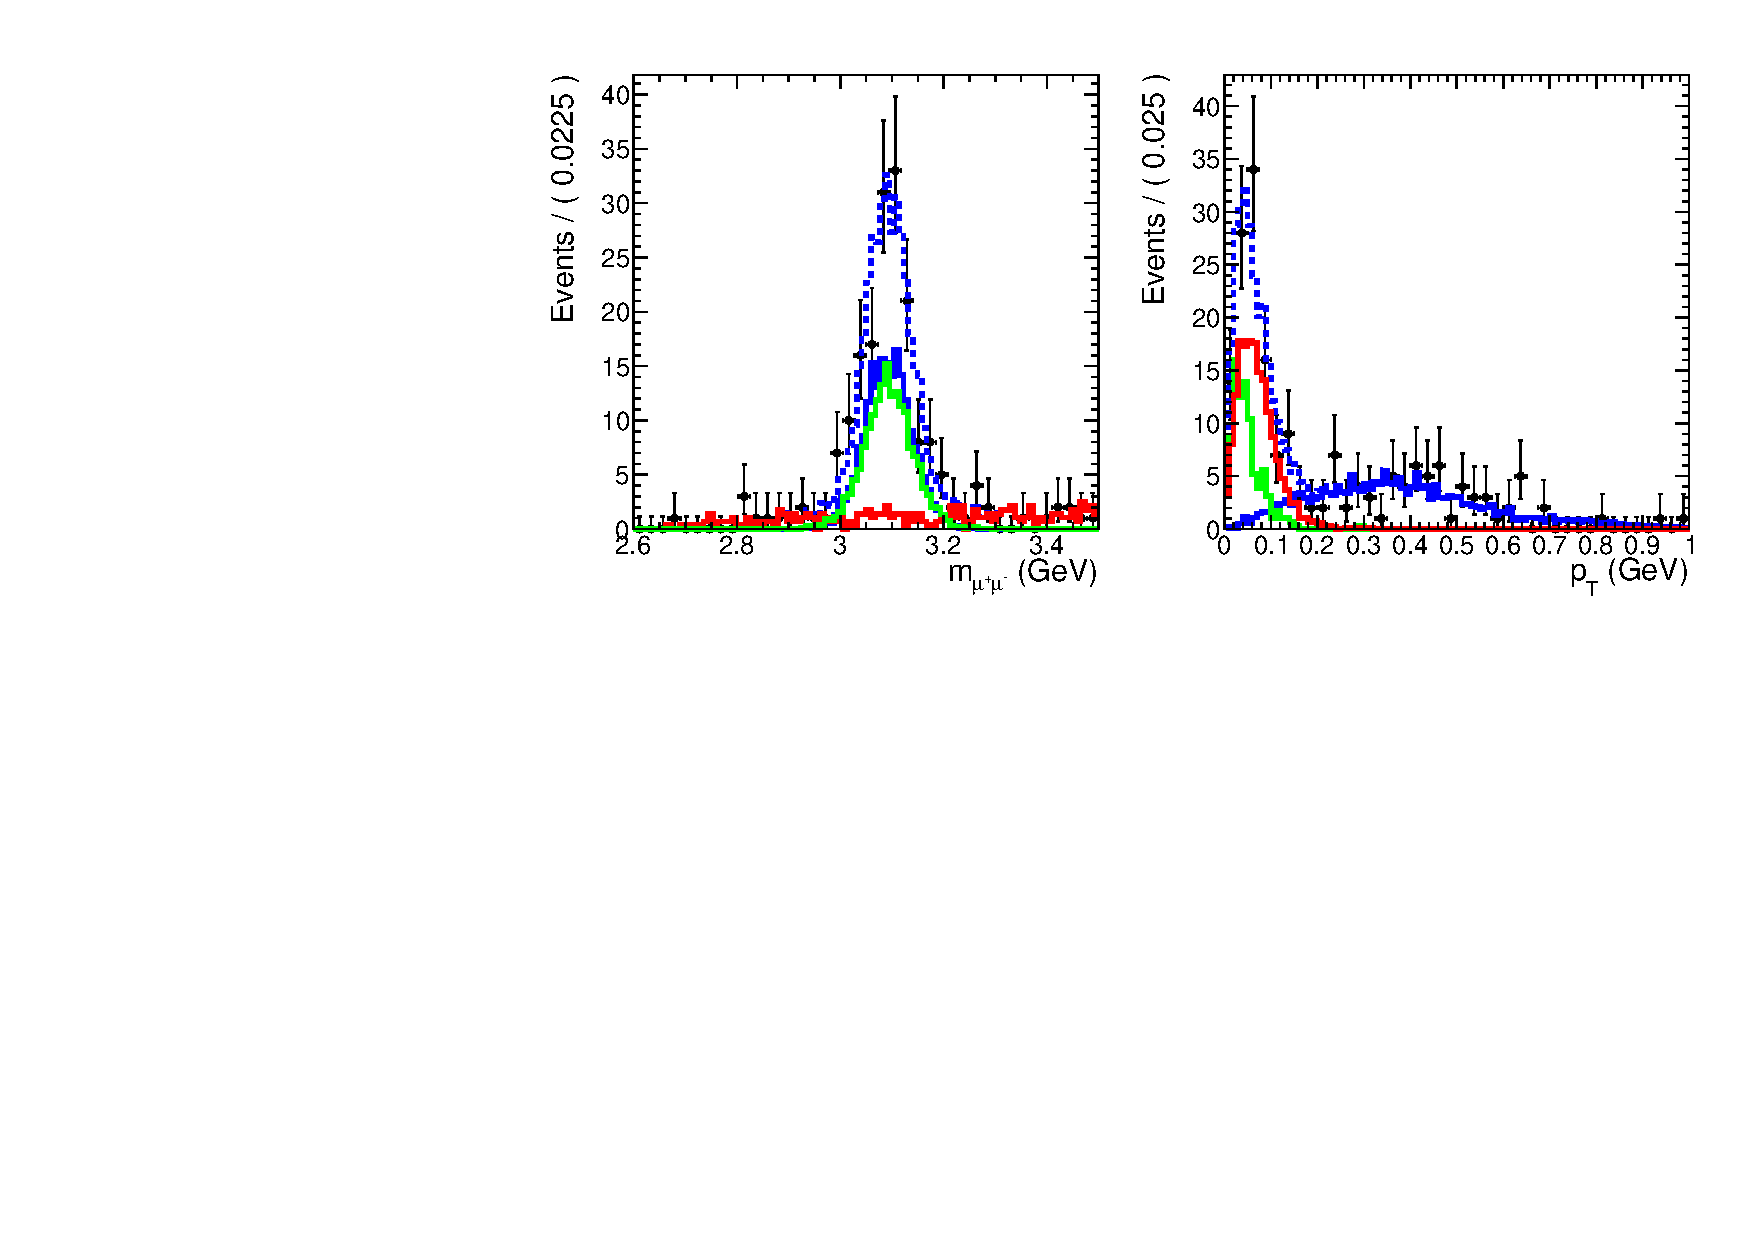
\includegraphics[width=0.6\textwidth]{ptMassSimTemp}
        \caption{Simultaneous fit to the mass and \pt{} using mass templates
          for the mass fit. }
        \label{fig:simFitTemp}
      \end{figure}

    \subsection{MC acceptance}
      The MC derived acceptance correction factors depend on the input physics
        generator. 
      The underlaying \pt{} distribution was assumed to be correctly 
        described by STARlight for the coherent cross section measurement.
      To estimate the effect of changing the underlaying \pt{} distribution 
        on the acceptance measured from the MC, the incoherent sample was used 
        to correct the coherent yield.
      By using the broader \pt{} distribution of the incoherent process, an 
        estimate of acceptance measurements dependence on the assumed shape of
        the \pt{} distribution was obtained.
      The systematic uncertainty due to the dependence of the acceptance 
        correction on the \pt{} distribution of the input physics generator
        was estimated by the difference between the correction factors from 
        the coherent and incoherent MC samples. 
      Half the difference was used as the estimate and was found to be 1.1\%.

      \begin{figure}[!Hhbt]
        \centering
        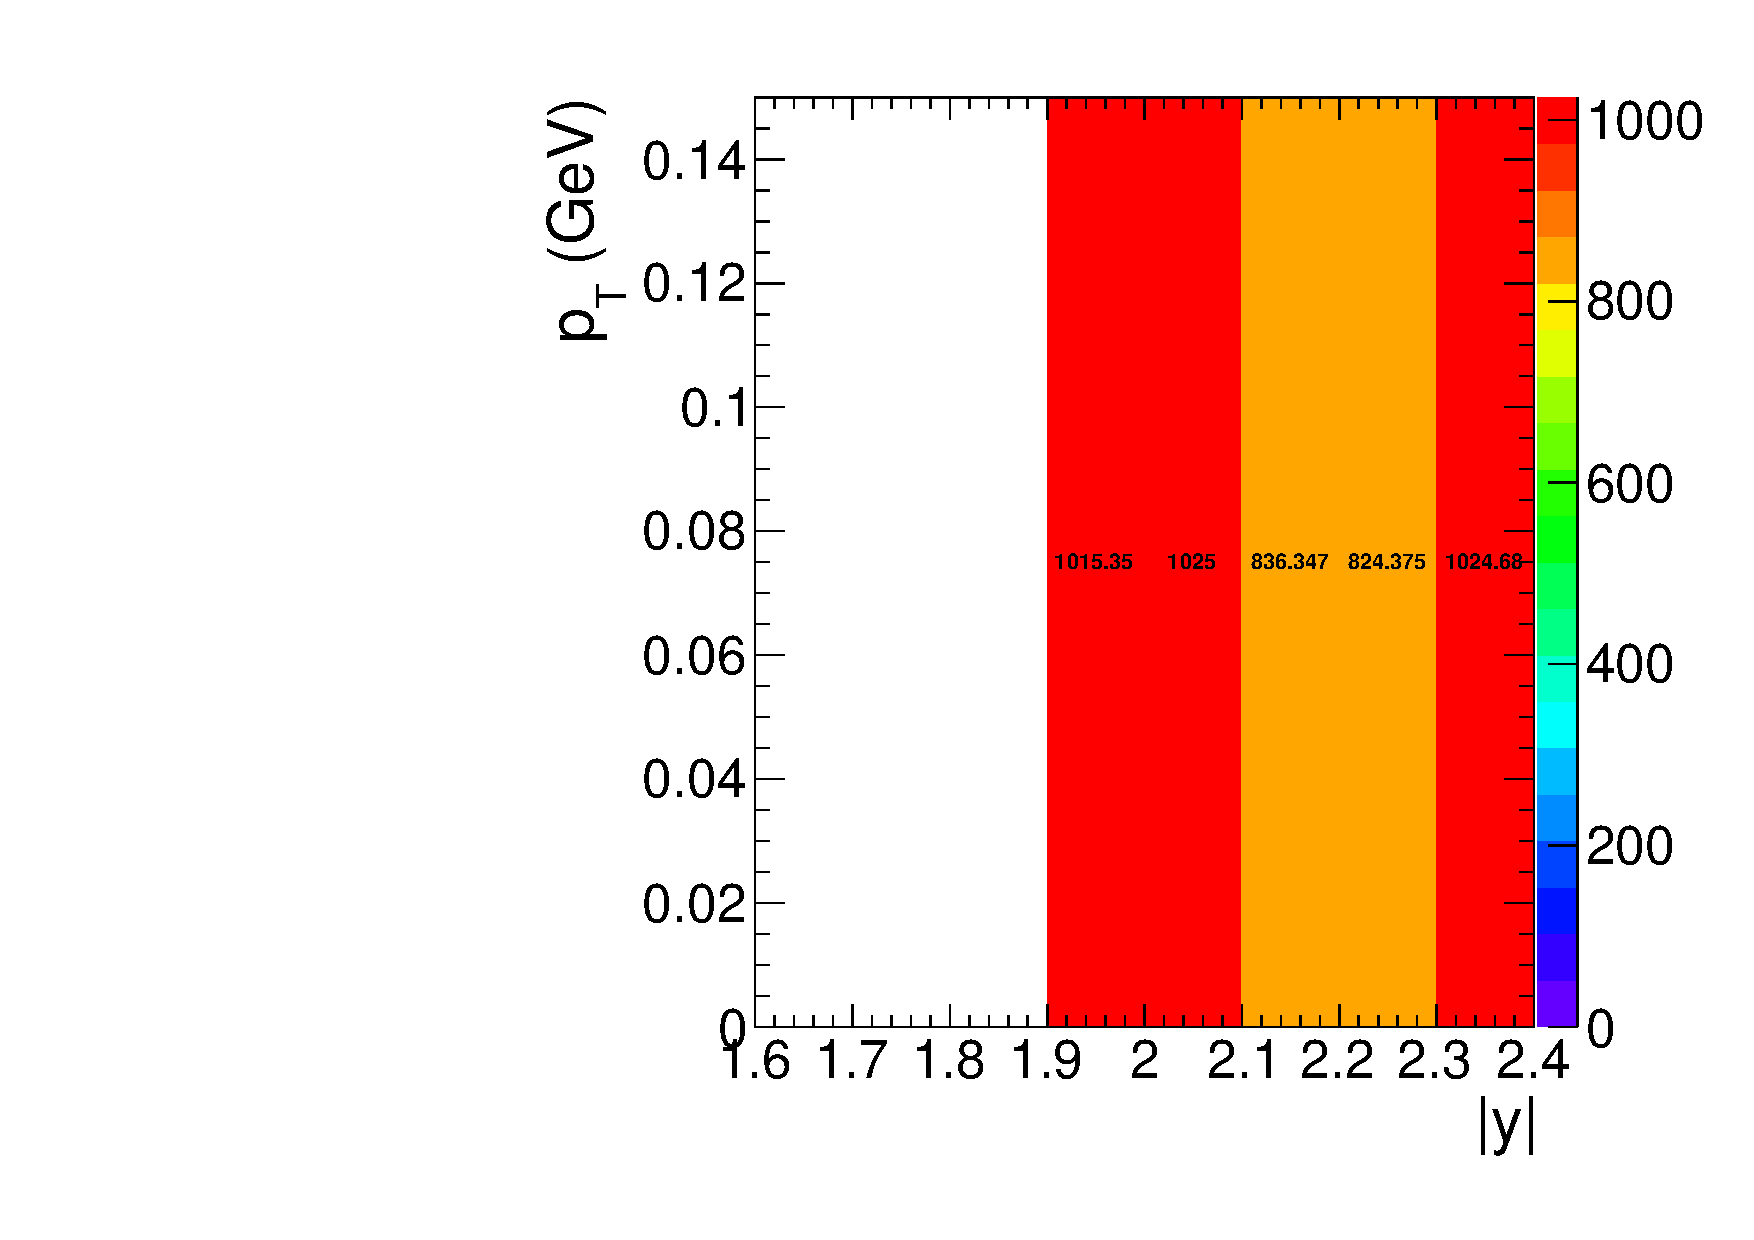
\includegraphics[width=0.6\textwidth]{coCorInCoAcc}
        \caption{Yields corrected by the MC incoherent acceptance map.}
        \label{fig:coYieldInCoCor}
      \end{figure}
      
      The effect of polarization was estimated by correcting by the acceptance
        for an unpolarized \JPsi{} sample.
      \begin{figure}[!Hhtb]
        \centering
        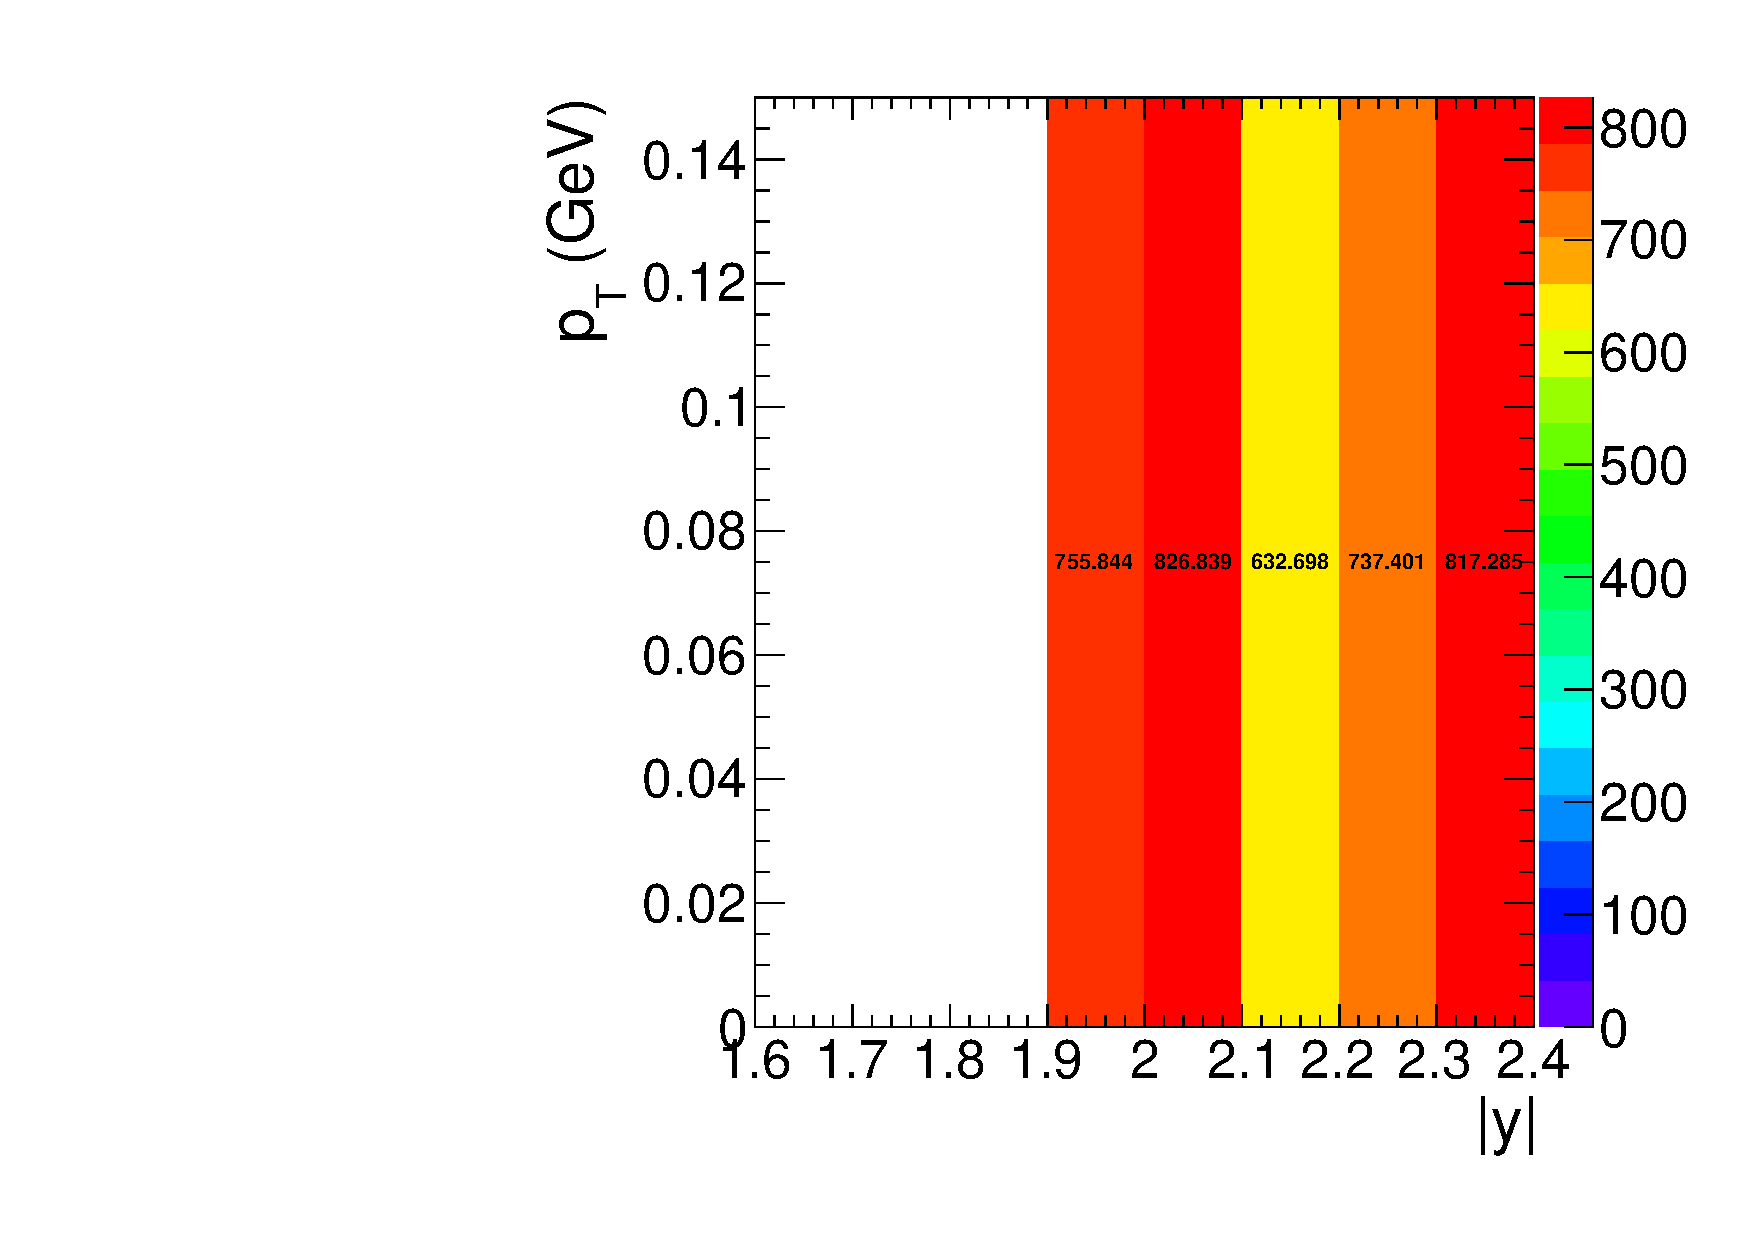
\includegraphics[width=0.6\textwidth]{coCoGaussGun}
        \caption{Yields corrected by an unpolarized \JPsi{} sample.}
        \label{fig:coYieldGaussCor}
      \end{figure}

    \subsection{ZDC reconstruction}
      An additional method for estimating the ZDC neutron thresholds was used
        to estimate the systematic errors on the threshold measurements.  
      This additional method, used in previous ZDC measurements, differs 
        in the way the signal time slices are used to calculate the signal from
        each channel.
      In the standard method, the signal is taken from the sum of time slices 
        4, 5, and 6.
      To estimate the event by event noise pedestal the sum of time slice 
        1 and 2 are used. 
      The signal for an individual ZDC channel is then calculated as the 
        sum of the signal time slices minus the sum of the noise time slices
        weighted by a factor of 3/2 to account for the differing number of 
        noise versus signal time slices.
      The advantage of the standard method is that by using multiple signal
        and noise time slices the signal and noise are effectively averaged
        reducing time slice to time slice fluctuations.
      However, by using time slices 1 and 2 for measuring the noise, the noise
        can only be measured half the time due to unmeasurable negative 
        fluctuations of the dominant low frequency component of the noise.
      
      As in the new method described in Section~\ref{sec:breakUpDet}, 
        the standard method combines the channels to create a signal 
        measurement from the whole of each side of the ZDC, one
        measurement for ZDC$^{+}$, and one for ZDC$^{-}$.
      The noise subtracted signal from each of the HAD channels are added 
        together.
      Then the EM section channels are summed. 
      The EM section is weighted by a factor of 0.1 as in the new method. 
      After the weighting the EM and HAD channels are added to each to create
        one measurement for ZDC$^{+}$ and another measurement for ZDC$^{-}$.
    
      Fig.~\ref{fig:zdcM1Fit} shows the spectra for ZDC$^{+}$ and ZDC${-}$ 
        using the standard method. 
      The same fit used for the new method is applied to standard method. 
      As in the new method, the single neutron threshold is set to 2$\sigma$
        below the mean from the fit to the one neutron peak.
      The multi-neutron threshold was set to 2$\sigma$ above the one neutron
        peak.

      \begin{figure}[!Hhtb]
        \centering
        $ \begin{array}{cc}
          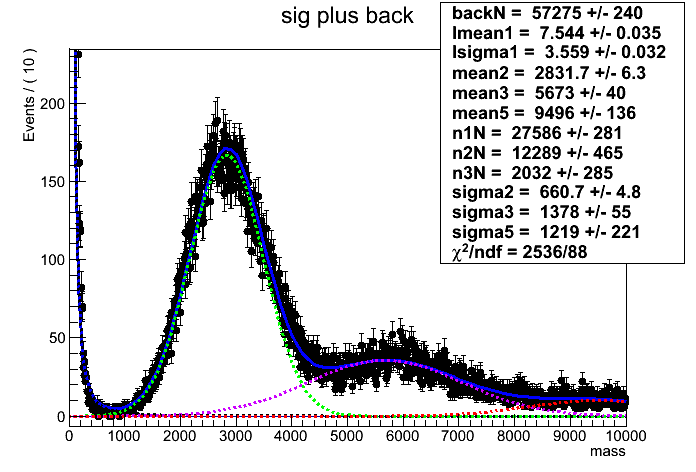
\includegraphics[width=0.45\textwidth]{zdcMinusZBFitTimeCut} &
          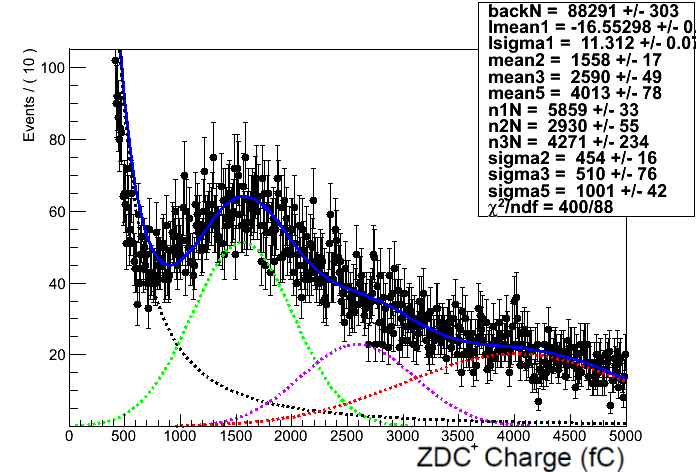
\includegraphics[width=0.45\textwidth]{zdcPlusZBFitTimeCut}
        \end{array} $
        \caption{Fit to charge spectrum from ZDC$^{-}$ (left) and ZDC$^{+}$ 
          (right) using the standard reconstruction method}
        \label{fig:zdcM1Fit}
      \end{figure}

      The systematic uncertainty due to the ZDC reconstruction method are
        estimated from the difference between the UPC \JPsi{} candidate yields.
      Both the reconstruction method and thresholds were changed to calculate 
        the effect of the reconstruction method.
      The yields for the new and standard ZDC reconstruction method in the Xn0n
        break up were found to be 298 and 315 respectively. 
      Half the difference between the two methods was used as an estimated of 
        the systematic uncertainty.
      The systematic uncertainty due to the ZDC reconstruction method was 
        found to be 2.9\%.

    \subsection{ZDC trigger efficiency}
      The ZDC trigger efficiency measurement is sensitive to the underlying 
        neutron distribution.
      The more neutrons that high the ZDC the higher the trigger efficiency 
        will be.
      To estimate the effect the input sample has on the efficiency, the ZDC 
        trigger efficiency was measured from five different samples.
      The Table~\ref{tab:zdcEfficiencySys} shows the results from the 
       five samples. 
      Both the new and standard ZDC reconstruction methods are shown for 
        comparison.

      \begin{table}
        \centering
        \begin{tabular}{|c|c|c|c|c|}
          \hline ZDC Side & Reco Method & N$_{events}$ & N$_{trig}$ & $\varepsilon_{ZDC}$ \\ \hline
           \multicolumn{5}{|c|}{(ZDC$^{+}$ or ZDC$^{-}$) and 1 pixel track} \\ \hline 
           ZDC$^{-}$ & 1 & 72946  & 71688 & 0.982 $\pm$ 0.005 \\ \hline
           ZDC$^{-}$ & 2 & 73028  & 71706  & 0.9819  $\pm$ 0.005  \\ \hline
           ZDC$^{+}$ & 1 & 76137  & 71786  & 0.9429  $\pm$ 0.005  \\ \hline
           ZDC$^{+}$ & 2 & 76132  & 71859  & 0.9439  $\pm$ 0.005  \\ \hline
           \multicolumn{5}{|c|}{(ZDC$^{-}$ or ZDC$^{+}$), 1 pixel track, and L1 EG trigger } \\ \hline 
           ZDC$^{-}$ & 1 & 613758  & 602123  & 0.9810 $\pm$ 0.0018 \\ \hline
           ZDC$^{-}$ & 2 & 614014  & 601863  & 0.9802 $\pm$ 0.0018 \\ \hline
           ZDC$^{+}$ & 1 & 643905  & 602671  & 0.9360  $\pm$ 0.0017 \\ \hline
           ZDC$^{+}$ & 2 & 647888  & 603089  & 0.9309  $\pm$ 0.0017 \\ \hline
           \multicolumn{5}{|c|}{(ZDC$^{-}$ or ZDC$^{+}$), 1 pixel track, and L1 Muon trigger} \\ \hline 
           ZDC$^{-}$ & 1 & 65466  & 63376  & 0.9681 $\pm$ 0.0054  \\ \hline
           ZDC$^{-}$ & 2 & 65543  & 63358  & 0.9667 $\pm$ 0.0054 \\ \hline
           ZDC$^{+}$ & 1 & 71929  & 63512  & 0.8830  $\pm$ 0.0048 \\ \hline
           ZDC$^{+}$ & 2 & 72932  & 63582  & 0.8718  $\pm$ 0.0047 \\ \hline
           \multicolumn{5}{|c|}{ Zero Bias with ZDC timing cuts} \\ \hline 
           ZDC$^{-}$ & 1 & 88676  & 84429  & 0.9521 $\pm$ 0.0046 \\ \hline
           ZDC$^{-}$ & 2 & 88480  & 84202  & 0.9517 $\pm$ 0.0046 \\ \hline
           ZDC$^{+}$ & 1 & 59878  & 54728  & 0.9140  $\pm$ 0.0054 \\ \hline
           ZDC$^{+}$ & 2 & 60467  & 54733  & 0.9052  $\pm$ 0.0053 \\ \hline
           \multicolumn{5}{|c|}{(ZDC$^{-}$ or ZDC$^{+}$)} \\ \hline 
           ZDC$^{-}$ & 1 & 30986 & 30333 & 0.9789 $\pm$ 0.0079 \\ \hline
           ZDC$^{-}$ & 2 & 31029 & 30339 & 0.9778 $\pm$ 0.0079 \\ \hline
           ZDC$^{+}$ & 1 & 39178 & 30164 & 0.7699 $\pm$ 0.0059 \\ \hline
           ZDC$^{+}$ & 2 & 35703 & 30443 & 0.8527 $\pm$ 0.0067 \\ \hline
           \multicolumn{5}{|c|}{ Zero Bias} \\ \hline 
           ZDC$^{-}$ & 1 & 109967  & 101598  & 0.9239 $\pm$ 0.0040 \\ \hline
           ZDC$^{-}$ & 2 & 110230  & 101561  & 0.9214 $\pm$ 0.0040 \\ \hline
           ZDC$^{+}$ & 1 & 253241  & 86660  & 0.3422 $\pm$ 0.0013 \\ \hline
           ZDC$^{+}$ & 2 & 156336  & 87401  & 0.5591 $\pm$ 0.0024 \\ \hline
        \end{tabular}
        \caption{ZDC trigger efficiencies for ZDC reconstruction method 1 and 
          2 for different trigger samples}
        \label{tab:zdcEfficiencySys}
      \end{table}
      
      The amount of electronic noise in the sample also effects the measurement.
      The more noise sits below the one neutron peak, the worse the efficiency 
        is. 
      In Table~\ref{tab:zdcEfficiencySys}, the Zero Bias sample compared the 
        Zero Bias sample with the timing cuts the described in the previous 
        section shows a significant increase in efficiency in the sample
        with reduced noise. 
      The same increase is seen when comparing the ZDC triggered sample with 
        the ZDC triggered sample that also requires a pixel track. 
      The effect of the electronic noise is also present in the difference seen
        in using the two methods.
      As seen in Fig.~\ref{fig:zdcSpec2v1}, the new reconstruction method 
        shows better separation of the one neutron peak from the electronic 
        noise, in particular in ZDC$^{+}$ where the signal gain is lower.
      For this reason, the Zero Bias data, which contains that largest 
        contribution from electronic noise, shows the most separation between 
        the two methods and give the lowest estimate for the ZDC trigger 
        efficiency.

      The systematic uncertainty due to the uncertainty in the 
        underlying distribution was estimated by calculating the standard 
        deviation of the least extreme values from 
        Table~\ref{tab:zdcEfficiencySys}.
      Any value greater than three standard deviations from the mean was thrown
        out. 

    \subsection{ZDC reconstruction method comparison}
      The new method relative to the standard method separates low signal from 
        the noise more effectively for both sides of the ZDC.
      This is particularly important for ZDC$^{+}$ where the 1st HAD section
        had a lower gain than the other sections. 
      The ZDC$^{+}$ and ZDC$^{-}$ signals near the one neutron peak using the
        standard and new reconstruction methods were plotted for comparison in 
        Fig.~\ref{fig:zdcSpec2v1}.
      \begin{figure}[h]
        \centering
        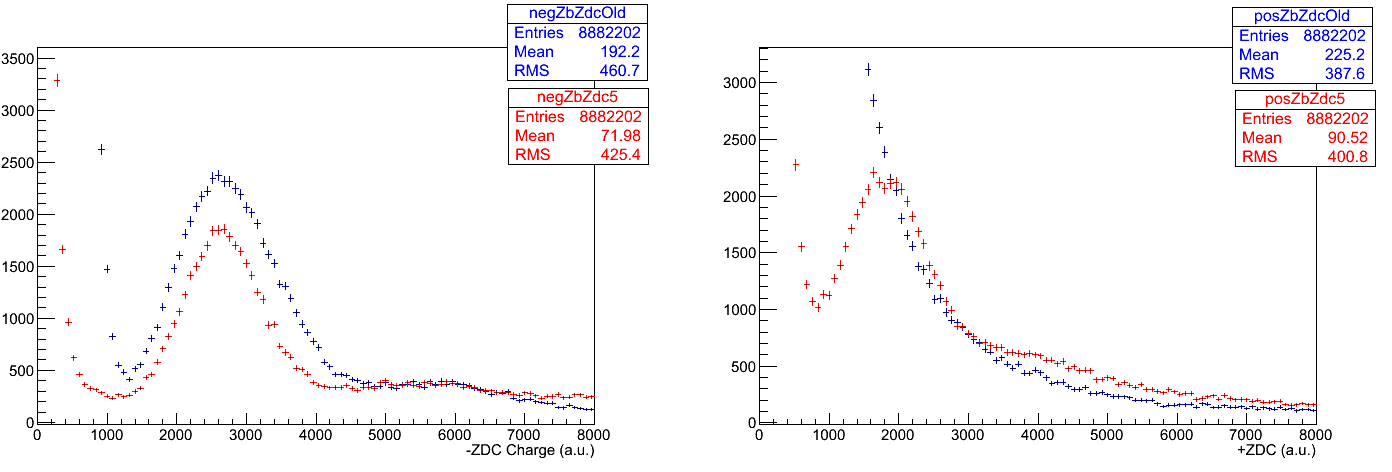
\includegraphics[width=\textwidth]{zdcSpec2v1}
        \caption{Comparison of the \textcolor{red}{new} ZDC reconstruction 
          method and the \textcolor{blue}{standard} method for ZDC$^{-}$ (left) and 
          ZDC$^{+}$ (right).}
        \label{fig:zdcSpec2v1}
      \end{figure}
      In Fig.~\ref{fig:zdcSpec2v1}, the shrinking of width of the noise peak 
        around zero in the new method versus the old method is apparent for
        both ZDC$^{+}$ and ZDC$^{-}$.
      For the standard method no single neutron peak is resolved in ZDC$^{+}$,
        whereas the single neutron peak is resolved using the new method. 

      Timing cuts were applied to enhance the signal relative to the background
        in order to resolve the one neutron peak in ZDC$^{+}$ using the 
        standard method. 
      Because the products of the collision are synced with time slice 4, noise
        can be rejected by selecting channels where the maximum signal falls 
        into time slice 4.
      The noise will have no preferred time slice (see Fig.~\ref{fig:zdcPulseShape}). 
      Using this fact, signal can be preferably selected by requiring that the
        hadronic channels of the ZDC have a peak signal in the fourth time 
        slice.
      Through these timing cuts the single neutron peak was recovered using the
       standard reconstruction for ZDC$^{+}$.

      To examine the effectiveness of the timing cuts, event by event noise 
        subtraction was removed from the standard reconstruction.
      The signal from each channel was taken from time slices 4,5, and 6 with
        out subtracting 1 and 2.
      The signal spectrum from ZDC$^{-}$ was then plotted with the result
        shown in Fig.~\ref{fig:zdcTimingCuts}.
      \begin{figure}[!Hhbt]
        \centering
        \includegraphics[width=0.6\textwidth]{zdcMinusSingleNuNoInc}
        \caption{Effects of requiring in-time signal in successively more 
          ZDC hadronic channels, no timing, at least \textcolor{red}{one}, at least \textcolor{green}{two},
            at least \textcolor{blue}{three}, and all \textcolor{yellow}{four} HAD channels have a maximum signal
            in the fourth time slice.}
        \label{fig:zdcTimingCuts}
      \end{figure}
      As each additional hadronic channel is required to have a maximum signal
        in the fourth time slice, the single neutron peak emerges. 
      Fig.~\ref{fig:zdcTimingCuts} demonstrates that the single neutron peak 
        can be recovered from the noise using timing cuts alone. 

      Using the standard noise subtraction method, the same signal that emerges
        from the timing cuts alone appear without timing cuts.
       \begin{figure}[h]
        \centering
        \includegraphics[width=0.6\textwidth]{zdcMinusSingleNuNoSub}
        \caption{Effect of ZDC signal timing requirements after noise 
          subtraction.}
        \label{fig:zdcTimingAfterNoiseSub}
      \end{figure}
      Fig.~\ref{fig:zdcTimingAfterNoiseSub} confirms that both noise 
        subtraction and the timing requirement produce the same signal.
      This gives confidence that the signal is not an artifact of either cut, 
        but the true neutron signal.

       Fig.~\ref{fig:zdcTimingAfterNoiseSub} and Fig.~\ref{fig:zdcSpec2v1} 
        demonstrate the consistence of the using timing cuts and noise 
        subtraction to enhance the signal neutron peak. 
      Fig.~\ref{fig:zdcTimingAfterNoiseSub} confirms the legitimacy of the 
        timing requirement method in ZDC$^{-}$ by showing the that the same
        signal emerges from the noise subtraction method as the timing method.
      Fig.~\ref{fig:zdcSpec2v1} demonstrates the corresponds between
        the new noise subtraction method and the standard method on in 
        ZDC$^{-}$ where signal is better separated from the electronic noise. 
      This allows for confidence that the signal seen in ZDC$^{+}$ using 
        the new method is the one neutron peak.
 
    \subsection{Tag and probe}
      The main purpose for fitting the mass spectra to estimate the efficiency
        is to separate the background from true signal. 
      The background may not have the same efficiency as the signal, so 
        separating the two is important if this is the case.
      In the tag and probe fit the signal peak from the \JPsi{} resonance
        is fit to the probes, passing probes, and failing probes alike (see
        Fig.~\ref{fig:tnpFitPlot}). 
      The signal shape, if from the same physical signal, will be 
        identical in each of the three distributions. 
      The background is for the passing and failing probes is fit using 
        different parameters for the background because the background
        may come from different physical processes than the signal or 
        non-physical sources like combinatorial backgrounds or misidentified
        fake particles.
      When the background comes from sources other than the physical signal,
        the background may give an efficiency estimate that is lower than
        the signal. 

      The trigger efficiency measured by the tag and probe method depend on
        the fitting functions use to estimate the background and signal 
        contributions. 
      Depending on what functions is used to fit the spectra, the amount of
        amount of background can be over or underestimated and effect the 
        efficiency measurement.
      To estimate this effect, the tag and probe efficiencies were additionally
        measured by counting probes in the \JPsi{} mass window. 
      The whole mass window is used to estimate the efficiency including all 
        the events from the mass side bands.
      In this way, a worst case scenario estimate is given where all background
        events are included as signal. 
      \begin{figure}[!Hhbt]
        \centering
        $ \begin{array}{cc}
          \includegraphics[width=.45\textwidth]{tNp/tnpCounting} &
          \includegraphics[width=.45\textwidth]{tNp/tnpFromFit}
        \end{array} $ 
        \caption{Tag and probe trigger efficiencies from counting (left) 
          compared to fitting (right)}
        \label{fig:tnpCntVFit}
      \end{figure}

      From Fig.~\ref{fig:tnpCntVFit} it is apparent that the choice of fit 
        function and therefore the amount of background from the mass side 
        bands is included in the signal measurement has very little effect on 
        the tag and probe efficiency measurement.
      The small effect of including the side bands is due to the side bands 
        being comprised mostly of photon-photon events.
      Because this background is neither decays from other particles like pions
        nor is it non-physical background like combinatorics, the efficiency
        for muons from the sidebands are nearly identical to \JPsi{} signal.
      The photon-photon process directly produces two muons just like the 
        \JPsi{}, therefore efficiency estimated from the side bands has 
        little effect on the measurement because of this similarity.
      The counting and fitting trigger efficiency measurements agree within 
        statistcal uncertainties, so this uncertianty was taken to be negliable.

    \subsection{MC vs Data compairson}
      \begin{figure}[h]
        \centering
        \includegraphics[width=0.5\textwidth]{jpsiMcComp/jpsiAbsRapCoherent}
        \caption{Comparison of the of the dimuon rapidity distributions between 
          coherent MC sample and Data.}
        \label{fig:jpsiAbsRapCoherent}
      \end{figure}
      \begin{figure}[h]
        \centering
        \includegraphics[width=0.5\textwidth]{jpsiMcComp/jpsiPhiCoherent}
        \caption{Comparison of the of the dimuon $\varphi$ distributions 
          between coherent MC sample and Data.}
        \label{fig:jpsiPhiCoherent}
      \end{figure}
      \begin{figure}[h]
        \centering
        \includegraphics[width=0.5\textwidth]{jpsiMcComp/jpsiPtCoherent}
        \caption{Comparison of the of the dimuon \pt{} distributions 
          between coherent MC sample and Data.}
        \label{fig:jpsiPtCoherent}
      \end{figure}


\chapter{Results} 
  The main results of this thesis are give here:
    the cross section for coherent \JPsi~production, the incoherent \JPsi~cross
    section, the cross section for muon pairs from photon-photon interactions,
    the ratio between break up mode yields, and the rapidity correlations 
    between dimuon candidates and neutrons in the ZDC.

  \section{Coherent cross section}
  The coherent cross section in calculated from the following equation:
  \begin{equation}
    \frac{d\sigma^{J/\psi}_{co}}{dy}  = \frac{N_{cor} f_{co}  }
    { \Delta y\mathcal{L}_{int} \varepsilon_{ZDC} \varepsilon_{p_{T}} 
      BR_{\mu^{+}\mu^{-}}}
    \label{eq:expXSecCo}
   \end{equation}
   where $N_{cor}$ is corrected dimuon yield, $f_{co}$ is the 
     fraction of events that come from the coherent process, 
     $BR_{\mu^{+}\mu^{-}}$ is the branching ratio for \JPsi~to $\mu^{+}\mu^{-}$, 
     $\varepsilon_{ZDC}$ is the efficiency for triggering the ZDC, 
     $\varepsilon_{p_{T}}$ is the efficiency for the 0.15 GeV cut in $p_{T}$, 
     $\mathcal{L}_{int}$ is the integrated luminosity, and $\Delta y$ is the 
     width the rapidity interval.

  The raw yield of dimuon candidates was measured after applying the cuts 
    described in Section~\ref{sec:DataSetEvSel}.
  \begin{figure}[!Hhtb]
    \centering
    \includegraphics[width=0.6\textwidth]{rawYield}
    \caption{Raw yield for the Coherent cross section measurement.}
    \label{fig:rawYieldCo}
  \end{figure}
  $N_{cor}$ was calculated by dividing the raw yields from 
    Fig.~\ref{fig:rawYieldCo} by the acceptance and efficiency factor from 
    Fig.~\ref{fig:avAccEff}, which combines $A$ and 
    $\varepsilon^{dimuon}_{trigger}$ as described in Section.~\ref{sec:effDet}.
  The corrected yields, $N_{cor}$, are shown in Fig.~\ref{fig:corYieldCo}.
  \begin{figure}[!Hhtb]
    \centering
    \includegraphics[width=0.6\textwidth]{correctedYieldAverage}
    \caption{Corrected yields for the coherent p$_{T}$ region.}
    \label{fig:corYieldCo}
  \end{figure}
  For the coherent cross section measurement, $N_{cor}$ is taken from the 
    region 2.0 < $|y|$ < 2.2 and $p_{T}$ < 0.15 GeV to avoid the edges of the
    detectors acceptance, bin migration in the calculation of $A$, and overlap
    between the coherent and incoherent process.
  From this procedure, the $N_{cor}$ was measured to be 1903.
  
  To measure $f_{co}$, the simultaneous fit shown in 
    Fig.~\ref{fig:simFitMassPtGauss} was used.
  The normalizations for each of the three components to the signal are fixed 
  by the fit as described in Section~\ref{sec:sigEx}.
  The normalized coherent template is integrated up to 0.15 GeV in $p_{T}$ and
    divided by the integral of the data $p_{T}$ spectrum up to 0.15 GeV.
  The statistical error taken from the fit, $f_{co}$ = 0.60 $\pm$ 0.11.

  The two efficiency terms, $\varepsilon_{ZDC}$ and $\varepsilon_{p_{T}}$, were
    measured from data and MC respectively.
  As described in Section~\ref{sec:breakUpDet}, $\varepsilon_{ZDC}$ was 
    measured in the from the ZDC triggered data set by dividing the number of 
    events both fire the ZDC trigger and pass the one neutron threshold.
  $\varepsilon_{ZDC}$ was measured to be 0.96 with a negligible statistical 
    error.
  The efficiency of the 0.15 GeV $p_{T}$ cut was estimated from MC by dividing 
    the number of events that are lost by applying the $p_{T}$ cut after all
    other cuts are applied. 
  From this method $\varepsilon_{p_{T}}$ = 0.95.
  
  The remaining two terms, $\mathcal{L}_{int}$ and $BR_{\mu^{+}\mu^{-}}$, 
    depend on Ref.~\cite{cmsLumi} and Ref.~\cite{pdg}.
  Ref.~\cite{cmsLumi} describes the method of using activity in HF to measure 
    the luminosity. 
  From this method, $\mathcal{L}_{int}$ was measured to be 143.3$\mu b^{-1}\pm$7.2.
  $BR_{\mu^{+}\mu^{-}}$ from Ref.~\cite{pdg} is 0.0593 $\pm$ 0.0006.
  From Equation~\ref{eq:expXSecCo}, $\frac{d\sigma^{J/\psi}_{co}}{dy}$ = 368 $mb$.

  \section{Incoherent cross section}
  The same basic procedure for measuring the coherent cross section was used to 
    calculate the incoherent cross section.  
  \section{Break up ratios}
    In Table~\ref{tab:r2} the ratio between raw yields for different break up 
      modes are shown.
    \begin{figure}[!Hhtb]
      \centering
      \includegraphics[width=.6\textwidth]{coherentBreakup}
      \caption{Ratio between J/$\psi$ yeilds XnXn and 1n0n break-up modes 
        compared the Xn0n break-up mode for J/$\psi$ with $p_{T}$ below 150 
        MeV.}
      \label{fig:coherentBreakUp}
    \end{figure}
   
    Fig.~\ref{fig:coherentBreakUp} and Fig.~\ref{fig:incoherentBreakUp} compare
      the raw break up ratios two STARlight and LTA predictions. 
    \begin{figure}[!Hhtb]
      \centering
      \includegraphics[width=.6\textwidth]{incoherentBreakup}
      \caption{Ratio between J/$\psi$ yeilds XnXn and 1n0n break-up modes 
        compared the Xn0n break-up mode for J/$\psi$ with 0.2 $< p_{T} <$ 
        1.5 GeV.}
      \label{fig:incoherentBreakUp}
    \end{figure}

    The number of the coherent and incoherent J/$\psi$ for each break-up mode are
      given in the Tab.~\ref{tab:r1}. 
    The ratios between the modes X$_{n}$X$_{n}$, 1$_{n}$0$_{n}$, 1$_{n}$1$_{n}$ and
      the mode  X$_{n}$0$_{n}$ are given in the table Tab.~\ref{tab:r2}. 
    Some of the  ratios can be obtained from  {\sc starlight} and from the Zhalov 
      and thus are given in Tab.~\ref{tab:r3}.
    \begin{table}[h]
      \begin{center}
      \begin{tabular}{|c|c|c|c|c|c|}
        \hline
         &  X$_{n}$0$_{n}$& X$_{n}$X$_{n}$ & 1$_{n}$0$_{n}$ & 1$_{n}$1$_{n}$  \\ \hline
        coherent J/$\psi$ &  242$\pm$16&94$\pm$10&58$\pm$8&8$\pm$3\\ \hline
        incoherent J/$\psi$ & 291$\pm$17&57$\pm$8&19$\pm$4&2$\pm$1\\ \hline
      \end{tabular}
      \caption{\label{tab:r1} Number of coherent J/$\psi$ integrated over $p_{T}$ and $y$ 
        with statistical uncertainty.}
      \end{center}
    \end{table}
    
    \begin{table}[h]
      \begin{center}
        \begin{tabular}{|c|c|c|c|c|}
          \hline
          & X$_{n}$X$_{n}$/X$_{n}$0$_{n}$ & 1$_{n}$0$_{n}$/X$_{n}$0$_{n}$ & 1$_{n}$1$_{n}$/X$_{n}$0$_{n}$  \\ \hline
          coherent J/$\psi$ &  0.39$\pm$0.05&0.24$\pm$0.04&0.03$\pm$0.01\\ \hline
          incoherent J/$\psi$ &  0.20$\pm$0.03&0.07$\pm$0.02&0.007$\pm$0.005 \\ \hline
        \end{tabular}
      \caption{\label{tab:r2} Number of coherent J/$\psi$ integrated over $p_{T}$ and $y$ 
        with statistical uncertainty.}
      \end{center}
    \end{table}

    In Table~\ref{tab:r3} the ratio between break up modes are shown for 
      different theories and processes.
    \begin{table}[h]
      \begin{center}
        \begin{tabular}{|c|c|c|c|c|}
          \hline
          & X$_{n}$X$_{n}$/X$_{n}$0$_{n}$ & 1$_{n}$0$_{n}$/X$_{n}$0$_{n}$ & 1$_{n}$1$_{n}$/X$_{n}$0$_{n}$  \\ \hline
          STARlight coherent &  0.37&-&0.02\\ \hline
          Zhalov coherent& 0.32&0.30&0.02\\ \hline
          STARlight incoherent &  0.37&-&0.007$\pm$0.02 \\ \hline
        \end{tabular}
        \caption{\label{tab:r3} Number of  J/$\psi$ integrated over $p_{T}$ and $y$ with 
          statistical uncertainty.}
      \end{center}
    \end{table}

  \section{diMuon-neutron correlations}
    In this section the correlation between the rapidity of the $\mu^{+}\mu^{-}$ 
      and of the neutron is studied. The following samples are studied: 
    \begin{itemize}
      \item $\gamma + A$ collisions in which two cases are considered
      \begin{itemize}
        \item elastic coherent interaction: here photon interacts with entier
          nucleus coherently and produce \JPsi. 
          Another photon is needed to cause the breakup and neutron emission. 
          Those two photons are uncorrelated and thus we don't expect to 
            observe the correlation between the rapidity of the neutron and the
            rapidity of the \JPsi.
          In the data sample this corresponds to the low-\pt \JPsi 
            (\pt$<$0.15~GeV). 
        \item inelastic incoherent interaction: here a single high \pt photoni
          interacting with nucleus produce the \JPsi and neutron. 
          The correlation between the rapidity of the neutron and the rapidity
            of the \JPsi is expected.
          In the data sample this corresponds to the high-\pt \JPsi 
            (0.15$<$\pt$<$1.05). 
      \end{itemize}
      \item $\gamma \gamma$ collisions: two photons collide and produce the 
        $\mu^{+}\mu^{-}$  and the third photon is needed to excite one of
          the nucleons and produce neutron. 
        Thus we don't expect to see the correlation between the rapidity of the
          neutron and the rapidity of the $\mu^{+}\mu^{-}$. 
        In the data sample this corresponds to the $\mu^{+}\mu^{-}$ with the
          invariant mass between 4 and 8~GeV. 
    \end{itemize}

    In order to study the correlation in rapidity between the neutron and
      dimuon direction we below four quantities and give they values in 
      Table~\ref{tab:corrneutronjpsi}.  
    \begin{itemize}
      \item $y^{-}_{\mu\mu} \wedge y_{n}^{-}$: number of $\mu^{+}\mu^{-}$ having
         $y<0$ and the neutron in ZDC$^{-}$ ($y<0$)
      \item $y^{-}_{\mu\mu} \wedge y_{n}^{+}$: number of $\mu^{+}\mu^{-}$ having
         $y<0$ and the neutron in ZDC$^{+}$ ($y>0$)
      \item $y^{+}_{\mu\mu} \wedge y_{n}^{+}$: number of $\mu^{+}\mu^{-}$ having
         $y>0$ and the neutron in ZDC$^{+}$ ($y>0$)
      \item $y^{+}_{\mu\mu} \wedge y_{n}^{-}$: number of $\mu^{+}\mu^{-}$ having
         $y>0$ and the neutron in ZDC$^{-}$ ($y<0$)
    \end{itemize}

    The ratio $R_{opp/same}$ is defined as: 
    \begin{equation}
      R_{opp/same} = \frac{y^{-}_{\mu\mu} \wedge y_{n}^{+} + y^{+}_{\mu\mu} 
        \wedge y_{n}^{-}}{y^{-}_{\mu\mu} \wedge y_{n}^{-} + y^{+}_{\mu\mu} 
        \wedge y_{n}^{+}}
    \end{equation}
    
    Ratios studied in this section are only sensitive to the difference between
      the ZDC$^{-}$ and ZDC$^{-}$.
    It is seen that the efficiency of both ZDCs in not exactly the same i.e.
      the efficiencies of ZDC$^{-}$ and ZDC$^{+}$ are respectively 
      $\varepsilon_{ZDC^{-}}$=0.98 and  $\varepsilon_{ZDC^{+}}$=0.94 and this 
      is taken in the account in the estimations. 
    The $R_{opp/same}$ radio corrected by the ZDCs efficiencies is also 
      included in Table~\ref{tab:corrneutronjpsi} and called 
      $R_{opp/same}^{\varepsilon_{ZDC}}$. 
    It is seen that the difference between corrected and uncorrected results is
      very small. 
    Other uncertainties cancel. 
    In this case cuts related to the acceptance and efficiencies corrections 
      are not necessary and thus they are released.
    
    Figure~\ref{fig:PtcorrandRation} gives \pt distributions of the \JPsi 
      when \JPsi and neutron have the opposite rapidity direction or when they 
      have the same rapidity direction for low-\pt and high-\pt \JPsi. 
    Also the Fig~\ref{fig:PtcorrandRation} gives the $R_{opp/same}$ for low-\pt
      and high-\pt \JPsi. 
    In is send from this plot that in the case of the low-\pt \JPsi this 
      $R_{opp/same}$ ratio is close to 1 and is decreasing when the \pt of
      \JPsi increases.
  
    \begin{figure*}[!Hhtb]
      \begin{center}
        \includegraphics[angle=0,width=0.45\textwidth]{cohOppAndSameNeutronDir}
        \includegraphics[angle=0,width=0.45\textwidth]{incohOppAndSameNeutronDir} \\
        \includegraphics[angle=0,width=0.45\textwidth]{ratiocohOppAndSameNeutronDir}
        \includegraphics[angle=0,width=0.45\textwidth]{ratioincohOppAndSameNeutronDir}
      \caption{ \label{fig:PtcorrandRation}  
        Transverse momentum distribution of the $J/\psi$ when  $J/\psi$ and 
          neutron have the opposite rapidity direction and the transverse 
          momentum distribution of the $J/\psi$ when  $J/\psi$ and neutron
          have the same rapidity direction for low-\pt (top left) and 
          high-\pt (top right) \JPsi. Bottom: Ratios $R_{opp/same}$ for 
          low-\pt ( left) and high-\pt ( right) \JPsi.}
      \end{center}
    \end{figure*}
    
    Compiled for \pt$<$1.05~GeV $R_{opp/same}$ ratio between the \pt 
      distribution of the \JPsi having neutron emitted in the opposite 
      direction and  the \JPsi having the neutron emitted in the same
      direction is shown on Fig.~\ref{fig:r2}. 
    \begin{figure*}[!Hhtb]
      \begin{center}
        \includegraphics[angle=0,width=0.65\textwidth]{RoppsameVsTheory}
        \caption{ \label{fig:r2} Ratio between the transverse momentum 
          distribution of the $J/\psi$ when  $J/\psi$ and neutron have 
          the opposite direction and the transverse momentum distribution 
          of the $J/\psi$ when  $J/\psi$ and neutron have the same direction.}
      \end{center}
    \end{figure*}
    The same distributions as~\ref{fig:PtcorrandRation} but now as a function 
      of rapidity of the \JPsi are presented in the Fig~\ref{fig:r3} and 
      compiled in Fig.~\ref{fig:r4}. 
    
    \begin{figure*}[!Hhtb]
      \begin{center}
        \includegraphics[angle=0,width=0.45\textwidth]{cohyOppAndSameNeutronDir}
        \includegraphics[angle=0,width=0.45\textwidth]{incohyOppAndSameNeutronDir}\\
        \includegraphics[angle=0,width=0.45\textwidth]{ratiocohyOppAndSameNeutronDir}
        \includegraphics[angle=0,width=0.45\textwidth]{ratioincohyOppAndSameNeutronDir}
        \caption{ \label{fig:r3} Rapidity distribution of the $J/\psi$ when  
          $J/\psi$ and neutron have the opposite rapidity direction and the 
          rapidity distribution of the $J/\psi$ when  $J/\psi$ and neutron 
          have the same rapidity direction for low-\pt (top left) and high-\pt 
          (top right) \JPsi. Bottom: Ratios $R_{opp/same}$ for low-\pt ( left) 
          and high-\pt ( right) \JPsi.}
      \end{center}
    \end{figure*}
    
    \begin{figure*}[!Hhtb]
      \begin{center}
        \includegraphics[angle=0,width=0.55\textwidth]{compiledratioincohandcohyOppAndSameNeutronDir}
        \caption{ \label{fig:r4} Rapidity ratios $R_{opp/same}$ for low-\pt 
          ( left) and high-\pt ( right) \JPsi.}
      \end{center}
    \end{figure*}
    
    Figure~\ref{fig:rNeutDimuCorr} shows the rapidity of the dimuon for the 
      events that are tagged by the ZDC$^{+}$ and  ZDC$^{-}$ means having 
      the neutron emitted in the $y>0$ and $y<0$. 
    
    \begin{figure*}[!Hhtb]
      \begin{center}
        \includegraphics[angle=0,width=0.42\textwidth]{ZDCDimuCorrCoh}\\
        \includegraphics[angle=0,width=0.42\textwidth]{ZDCDimuCorrIncoh}\\
        \includegraphics[angle=0,width=0.42\textwidth]{ZDCDimuCorrGammaGamma}
        \caption{ \label{fig:rNeutDimuCorr} Rapidity distribution of \JPsi in the
          case of the events having the neutron in negative and positive rapidity 
          for the low-\pt \JPsi (top), high-\pt \JPsi (middle) and dimuons from
          $\gamma \gamma$ sample (bottom). }
      \end{center}
    \end{figure*}
    
    Another, interesting correlation between the \JPsi rapidity direction and 
      the neutron rapidity can be also studied with quantities defined in 
      Eq.~\ref{eq:Ration} that are calculated in the 
      Table~\ref{tab:corrneutronjpsi}. 
    Table~\ref{tab:corrneutronjpsieffcorr} gives the same quantities as  
      Table.~\ref{tab:corrneutronjpsi} but here it is corrected for the 
      difference between the efficiency of the ZDC$^{+}$ and  ZDC$^{-}$. 
    
    \begin{equation}
      \label{eq:Ration}
      R_{(\mu\mu)^{-}}^{n^{-}/n^{+}} =  \frac{y^{-}_{\mu\mu} \wedge 
        y_{n}^{-}}{y^{-}_{\mu\mu} \wedge y_{n}^{+} }~~~~~~~~\mbox{and}~~~~~
        R_{(\mu\mu)^{+}}^{n^{-}/n^{+}} =  \frac{y^{+}_{\mu\mu} \wedge 
        y_{n}^{-}}{y^{+}_{\mu\mu} \wedge y_{n}^{+} }
    \end{equation}
    
    \begin{table}[h]
      \begin{center}
        \begin{tabular}{|c|c|c|c|c|c|c|}
          \hline
          & $y^{-}_{\mu\mu} \wedge y_{n}^{-}$ & $y^{-}_{\mu\mu} \wedge y_{n}^{+}$ 
          & $y^{+}_{\mu\mu} \wedge y_{n}^{+}$ & $y^{+}_{\mu\mu} \wedge y_{n}^{-}$ 
          & $R_{(\mu\mu)^{-}}^{n^{-}/n^{+}}$ 
          & $R_{(\mu\mu)^{+}}^{n^{-}/n^{+}} $  \\ \hline
          low-\pt \JPsi & \textcolor{blue}{78 $\pm$ 8.8} 
          & \textcolor{blue}{47 $\pm$  6.8}  & \textcolor{blue}{81 $\pm$  9}  
          & \textcolor{blue}{74 $\pm$  8.6} & \textcolor{blue}{ 1.66$\pm$0.31  } 
          & \textcolor{blue}{ 0.91$\pm$0.15  } \\ \hline
          high-\pt \JPsi & \textcolor{blue}{132 $\pm$  11.5}  
          & \textcolor{blue}{17 $\pm$  4.1}  & \textcolor{blue}{117 $\pm$  10.8}  
          & \textcolor{blue}{29 $\pm$  5.4} & \textcolor{blue}{7.76$\pm$2.0} 
          & \textcolor{blue}{0.25$\pm$0.05 } \\ \hline
          $\mu^{+}\mu^{-}$ from $\gamma \gamma$ & \textcolor{blue}{80 $\pm$8.9} 
          & \textcolor{blue}{81 $\pm$9} & \textcolor{blue}{75 $\pm$8.7} 
          & \textcolor{blue}{83 $\pm$9.1} & \textcolor{blue}{0.99$\pm$0.16 } 
          & \textcolor{blue}{1.11$\pm$0.18} \\ \hline
        \end{tabular}
        \caption{\label{tab:corrneutronjpsi} Number of dimuon pairs for 
          different directions of the neutron rapidity direction together with 
          $R_{(\mu\mu)^{-}}^{n^{-}/n^{+}}$ and 
          $R_{(\mu\mu)^{+}}^{n^{-}/n^{+}}$.}
      \end{center}
    \end{table}
    
    \begin{table}[h]
      \begin{center}
        \begin{tabular}{|c|c|c|}
          \hline
          & $R_{(\mu\mu)^{-}}^{\varepsilon_{ZDC}(n^{-}/n^{+})}$ 
          & $R_{(\mu\mu)^{+}}^{\varepsilon_{ZDC}(n^{-}/n^{+})} $  \\ \hline
          low-\pt \JPsi &  \textcolor{blue}{1.59 $\pm$ 0.29} 
          & \textcolor{blue}{0.88 $\pm$ 0.14} \\ \hline
          high-\pt \JPsi  & \textcolor{blue}{7.45 $\pm$ 1.87}  
          &  \textcolor{blue}{0.24 $\pm$ 0.05 } \\ \hline
          $\mu^{+}\mu^{-}$ from $\gamma \gamma$ 
          & \textcolor{blue}{0.95 $\pm$ 0.15} 
          & \textcolor{blue}{ 1.06 $\pm$ 0.17 } \\ \hline
        \end{tabular}
        \caption{\label{tab:corrneutronjpsieffcorr} Ratios 
          $R_{(\mu\mu)^{-}}^{\varepsilon_{ZDC}(n^{-}/n^{+})}$ and 
          $R_{(\mu\mu)^{+}}^{\varepsilon_{ZDC}(n^{-}/n^{+})} $ 
          i.e. $R_{(\mu\mu)^{-}}^{n^{-}/n^{+}}$ and 
          $R_{(\mu\mu)^{+}}^{n^{-}/n^{+}} $ corrected by the ZDC$^{+}$ and
          ZDC$^{-}$ efficiencies.}
      \end{center}
    \end{table}
    
    Integrated over rapidity, separately for $y<0$ and $y>0$ ratios from 
      Table~\ref{tab:corrneutronjpsieffcorr} are shown in the 
      Figure~\ref{fig:integRatios}.
    
    \begin{figure*}[!Hhtb]
      \begin{center}
        \includegraphics[angle=0,width=0.52\textwidth]{RCompiledYCorr}
        \caption{ \label{fig:integRatios} 
          $R_{(\mu\mu)^{-}}^{\varepsilon_{ZDC}(n^{-}/n^{+})}$ and 
          $R_{(\mu\mu)^{+}}^{\varepsilon_{ZDC}(n^{-}/n^{+})}$ integrated over 
          one side in rapidity for low- and high-\pt \JPsi and also for dimuons
          from $\gamma \gamma$ sample. }
      \end{center}
    \end{figure*}
    
    From the Tab~\ref{tab:corrneutronjpsi} and the Fig.~\ref{fig:rNeutDimuCorr} 
      it is seen as expected that there is no correlation between the \JPsi 
      rapidity and neutron rapidity in the case of the low-\pt \JPsi and 
      dimuons coming from $\gamma \gamma$ sample. 
    In the case of the high-\pt \JPsi the correlation is clearly visible.  

\chapter{Summary}
  As physicists' understanding of the QGP has deepened over the past 30 years
    of doing experimental heavy ion physics, the questions surrounding the
    QGP have shift from the confirmation of creation of a deconfined state
    to understanding the properties of the state that is created.
  It appears that the QGP is a hot nearly viscosity free fluid of strongly 
    coupled quarks and gluons. 
  The control measurements from dAu collisions at RHIC, and pPb collisions
    at the LHC have shown signs of collective behavior such as flow, which 
    made these results difficult to interpret.
  Additional knowledge of the initial state of the colliding nuclei is needed
    in order to fully understand the QGP signal seen in PbPb and AuAu 
    collisions.
  UPC events can provide this needed knowledge. 
  This thesis contributes to the understanding of the initial state through
    the measurement of the UPC \JPsi{} photoproduction cross section. 

  Ultra-peripheral collisions are clean probe of the initial state. 
  In UPC \JPsi{} photoproduction, the nuclei interact through the 
    electromagnetic force precluding the possibility of creating a collective
    medium.
  The theoretical models of coherent UPC \JPsi{} photoproduction model these 
    electromagnetic interactions by combining a semi-classical calculation 
    of the photon flux with a variety of phenomenological and QCD based 
    calculations of the nuclear gluon density. 
  The Wis\"{a}cker-Williams approximation \cite{WWFermi} is used to calculate 
    the flux of photons that surround the colliding nuclei. 
  The interaction of these photons with the nucleus is either calculated 
    through a nuclear modification of the proton gluon density 
    \cite{pQCD2013.02, lta2012.03}, or by modeling the nucleus as a collection
    of nucleons and scaling the nucleon photoproduction cross-sections from 
    e-p collisions \cite{vmd1999}, a Glauber model approach. 
  Photoproduction cross sections from from UPC events can determine at what 
    energy scale the Glauber based method breaks down.
  For the gluon density based calculations, there is a wide descrepancy 
    between the predictions, and photoproduction cross sections constrain which
    gluon density models are viable. 

  In this thesis, the CMS detector was used to measure the coherent UPC \JPsi{} 
    photoproduction cross section.
  The all of the three  major subsystems of CMS were used, the tracker, 
    the muon system, the calorimeter system, were used.
  The tracker records the position charge excitations in the silicon due to 
    particle hits, which are used to reconstruct the trajectory of charged 
    particles. 
  The muon system is comprised of the three gaseous detectors, the DTs, the 
    RPC, and the CSCs, which record charge deposits as high momentum particles
    ionize the gass within the detector.
  The muon system primary purpose is for triggering on and identifying muons.
  The calorimeter system measures the energy of deposited by particle induced
    showers as a means of reconstructing neutral particles and jets.
  
  The analysis in this thesis consists of three major components, development
    of a trigger, estimation of efficiency, and measurement of signal events.
  The trigger development involved designing a trigger based on rate estimates
    from past data that ensured a sample that could be used for both measuring
    the signal and estimate the efficiency of the trigger, reconstruction, and
    event selection.
  The number signal \JPsi{} candidates was measured by first applying a set 
    of event selection cuts that rejected background events such as hadronic
    collisions and beam gas collisions, then fitting the remaining events to
    templates from simulation to separate the three remaining physics processes,
    the coherent, incoherent, and photon-photon process.
  The efficiencies for each part of the trigger were measured from data. 
  The acceptance and reconstruction efficiency were estimated from MC.
  The cross section was calculated by combining the efficiency with the 
    measured luminosity and number of coherent \JPsi{}.
  The statistical uncertainties were taken from the template fit.
  The systematic uncertainties were estimated by varying the method used on 
    each component of the analysis. 

  The UPC \JPsi{} photoproduction cross section, $\frac{d\sigma^{J/\psi}_{co}}{dy}$,
    was found to be \textcolor{red}{368 $\pm$ 38 $\mu$b}. 
  When rescaled by a factor of 5.06 to account for the difference of break-up mode between 
    the measurement in this thesis and the ALICE result in Ref.\cite{alice2012.09}, the 
    result of \textcolor{red}{1.86 $\pm$ 19 mb} was found to be consistent with the 
    predictions in Ref.\cite{pQCD2013.02} of \textcolor{red}{1.8 mb}.  
  The calculation in Ref.\cite{pQCD2013.02} is also favored by the ALICE measurements. 
  Of the gluon distributions used in Ref.\cite{pQCD2013.02}, a gluon distribution with 
    moderately strong gluon shadowing, EPSO9, is consistent with both the results from this
    thesis and the previous ALICE results. 
  This indicates that at the scale of the mass of the \JPsi{} the nucleus gluon density is 
    significantly suppressed compared to the gluon densities of a nucleon.
  At this scale the nucleus can not be represented as a collection of nucleons as in the 
    Glauber like model described in Ref.\cite{vmd1999}.

  The measurement in this thesis confirms the ability to increase the knowledge of the 
    initial state though the exploration of UPC events. 
  This confirmation opens the door to additional measurements in this growing field of UPC
    research.
  A whole host of measurements will be possible with the data already recorded and will be
    recorded in the coming years by CMS and the other LHC experiments. 

  Ultra-peripheral heavy ion collisions provide an opportunity to study 
    the nature of the initial state. 
  Model calculations of the nuclear gluon density can be constrained by 
    studying quarkonia photoproduction at the LHC.
  In this thesis, the coherent \JPsi{} photoproduction cross section in 
    ultra-peripheral PbPb collisions at $sqrt(s_{NN})$ = 2.76 TeV.
  This was done by analysing data from the 2011 PbPb run recorded by the CMS 
    detector.
  A brief description of the detector apparatus was presented in this thesis.
  A special set of triggers was developed for the analysis in this thesis.
  These events are characterized by low \pt{} dimuons.
  Although the CMS detector was not designed to study this type of event, the
    analysis in this thesis demonstrates how versatile CMS can be at handling 
    both low \pt{} and low multiplicity events. 
  However, this analysis suffers from small statistics. 
  This is due to low acceptance for triggering on low \pt{} muons as well as 
    the difficulty to trigger these muons in coincidence with neutrons in the 
    ZDC.
  
    
  

\chapter{Future Works}  
  \section{Studies of 2011 PbPb data}

    \subsection{High mass $\gamma-\gamma \rightarrow e^{+} e^{-}$  in PbPb 2011}
      A study of the di-electron production in UPC events is already possible 
  from the recorded 2011 data. 
      This measurement would make use of the electron triggers and combined the 
  current di-muon data with di-electron data from the triggers using the
  ECAL. 
      The electron triggered sample potentially offers a large increase in 
  statistics. 
      By adding the additional channel the statistics would already increase.
      However in addition to this, because of the smaller mass of the electron,
  di-electron production is slightly favor compared to di-muon 
  production.
      STARlight predicts that di-electron cross section is a factor of more than 
  2.5 higher in Xn break-up mode than the di-muons channel when looking 
  at masses above 4 GeV.
      The acceptance for electrons in potential higher as well. 
      The ECAL is position just beyond the tracker, whereas the muon system is 
  outermost sub-detector. 
      This elevates the main reduction of muon acceptance, which is the material
  budget. 
      There is simply a lot a detector in front the muon system.

      In order to perform the study several key additions would need to be made
  relative to the current di-muon analysis. 
      The original reconstruction of the data used in the current di-muon 
  analysis does not contain electron objects. 
      Either the analysis would have to migrated to reconstruction of the data
  done in a newer software version, or reconstruction of the electrons 
  would have to be added to the current analysis chain. 
      There are currently no electron UPC MC samples produced. 
      In order to study the acceptance and efficiency for electrons these samples
  would be need. 
      The ultimate limitation on this study is the 2 GeV threshold in $p_{T}$ in
  the ECAL trigger. 
      This limits the di-electron mass range to where the trigger is efficient. 

      The contribution of higher order diagrams can be explored by the 
  photoproduction of di-lepton pairs is to explore.
      With additional contributions to the physics communities understanding of 
  this process this study will help to determine necessity or 
  non-necessity of including higher order of corrections in simulations 
  such as STARlight.
      Having an additional channel to help constrain the current di-muon measure 
  of the of UPC $\gamma-\gamma$ interaction will also help to constrain 
  the $J/\psi$ measurement by adding a data driven check on the 
  normalization $\gamma-\gamma$ background to the $J/\psi$
      
    \subsection{UPC Hadronic Overlap and PbPb 2011}
      In the model calculations explored in this analysis of UPC quarkonia 
        photoproduction all hadronic interactions are rejected.
      Photoproduction in events where hadronic interactions occur are not 
        included in the cross section calculation.
      However, inclusive $p_{T}$ spectra of $J/\psi$ measured by ALICE in 
        peripheral PbPb collisions show a low momentum peak consistent with 
        coherent photoproduction ~\cite{aliceIclJpsi}.
      \begin{figure}[h]
        \centering
        \includegraphics[width=0.5\textwidth]{2012-Sep-24-excess7090.pdf}
        \caption{Coherent excess in inclusive $J/\psi$ $p_{T}$ spectrum.}
        \label{fig:alicePtSpecLowPt}
      \end{figure}
      CMS has the opportunity to explore this overlap between hadronic 
        interactions and photoproduction using PbPb data from 2011 that is 
        already recorded.

      To study the overlap between photoproduction and hadronic proctuction of 
        quarkonia event the inelastic sample and the UPC sample could both be
        used. 
      The looseness of the veto designed to reject hadronic interactions,
        which uses the BSC detector, leaves a significant overlap with 
        peripheral hadronic collisions. 
      The inclusive quarkonia sample from typical hadronic collisions can also 
        be utilized. 
      Coherent quarkonia photoproduction has a distinctive low $p_{T}$ structure
        that can be used to identify photoproduced candidates in a sample that 
        contains photoproduction combined with hadronic interactions.
      This measurement would open up the door to exploring the boundary between
        photoproduction and hadronic production.
      By looking at the mixing of the two, both process, hadronic production and 
        photoproduction, will be better understood.

      In order to compliment each others strengths, the inclusive hadronic sample 
        and the UPC sample of dimuon candidates would be utilized in this study.
      The two samples muon and centrality biases are orthogonal allowing each to 
        serve as a check on the other. 
      The inclusive hadronic sample is triggered by a higher $p_{T}$ threshold 
        double trigger, whereas the UPC sample is uses a lower $p_{T}$ single 
        muon trigger.
      The UPC sample is strongly biased toward peripheral events, which would 
        lead to inefficiencies as events become more central, whereas, the 
        inclusive sample is slightly biases in the most peripheral events due to
        an inefficiency an event selection efficiency in the most peripheral 
        centrality bin.
      If these offsetting biases can be exploited, clarity about the transition 
        between and mixing of photoproduction and hadronic production of 
        quarkonia can be produced. 
      A measurement of the kind proposed here will both produce a better 
        understanding of the low $p_{T}$ portion of the inclusive spectrum as 
        well as the hadronic overlap with UPC measurements.

    \subsection{UPC with muons in HF}
      As higher rapidities are explored both lower and higher momentum partons
        of the nucleus are probed. 
      Because these two contributions to the UPC photoproduction cross section 
        can be separated using neutron tagging in incoherent events, exploring
        higher dimuon rapidities becomes attractive.
      HF extends to 5 in $\eta$, 2.6 units beyond the edge of the tracker.
      By combining hits in HF with tracks in the tracker the higher dimuon 
        rapidities could be explored. 
      When combined with neutron tagging of incoherently produced quarkonia,
        the current study can be extended to probe lower-x nuclear partons 
        by identifying muons in HF. 

  \section{Studies of 2013 pPb data and 2015 PbPb data}
    Specific UPC triggers were also developed for the pPb run in 2013. 
    For this period of running a much higher total trigger rate was read out 
      relative to 2011.
    The total rate allocated for UPC triggers at the L1 in 2013 was 5kHz and 
      50 Hz at the HLT.
    This factor of 5 increase in the bandwidth, especial in L1 rate, allowed for
      a different triggering strategy than in 2011. 

    The basic strategy in 2013 was the same as in 2012, use the loosest 
      available ECAL and muon L1 triggers to push to capture the lowest $p_{T}$
      electrons and muons possible paired with a veto on hadronic interactions,
      but was impemented differently.
    Because of the L1 bandwidth restrictions in 2011, both the ZDC and the BCS 
      were used on the L1 to reduce rates.
    In 2013 only the muon and ECAL triggers were used on the L1 allowing for 
      rejection of hadronic interactions through cuts on track multiplicity. 
    In addition, a more sophisticated trigger using full dimuon reconstructed 
      was developed to increase purity.
    The main advantage in this shift in strategy was a higher purity due to 
      the increased sophistication of the reconstruction on the HLT.
    In addition, an increase in cross section of the underlying physics process
      was achieved by relaxing the neutron emission requirement.

    The PbPb run in 2015 will be at higher beam energies and luminosities.
    The $sqrt{s_{NN}}$ will increase from 2.76 TeV in 2011 to 5.1 TeV with
      a project integrated luminosity between $0.3/nb$ and $1/nb$. 
    The factor of 2 to 10 increase in integrated luminosity will increases the 
      number of events directly.
    In addition, both the increase in energy, which increases the photon flux,
      and the ability to utilize the 2013 trigger strategy of sifting the 
      onus of the trigger selection to the HLT will increase the measured 
      yields relative to 2011.
    The higher beam energy, higher integrated luminosity, and added selectivity
      of the HLT will create the opportunity to explore both $J/\psi$ with 
      greater statistical precision and novel objects such as $\Upsilon$, and 
      jets. 

    \subsection{pPb $J/\psi$}
      $J/\psi$ photoproduciton in pPb collisions is dominated $\gamma-p$ 
        interactions.
      The measurement would primarily probe the proton gluon densities.
      In Eq.~\ref{eq:photonFluxFinaltmp} the photon flux depends on the square
      of the number of protons in parent nucleus, $Z^{2}$. 
      However, the cross section of the target only increase as the total 
        number of nucleons to the 2/3rds power, $A^{2/3}$.
      The much higher photon flux from the Pb ion more than compensates for 
        the decreased size of the proton.

      A pPb UPC $J/\psi$ measurement will compliment the measurements done at 
        HERA, and measurements done by ALICE.
      CMS will contribute by adding additional kinematic coverage and cover a 
        unique range of proton-photon center of mass energies, $W_{p\gamma}$. 
      The difference in beam energies and species at LHC versus HERA result in
        access to different $W_{p\gamma}$. 
      ALICE and CMS have different acceptance in $J/\psi$ rapidity, which also 
        translates to coverage of different $W_{p\gamma}$.
      In addition, an excess in the UPC cross section compared to HERA 
        measurements would indicate a non-exclusive contribution to the pPb UPC 
        $J/\psi$ cross section. 
      This measurement will both help enhance the current understanding of 
        the $p\gamma$ $J/\psi$ photoproduction cross section as a function of 
        $W_{p\gamma}$, and validate the UPCs measurements as an extension of 
        the work done at HERA.

    \subsection{UPC $J/\psi$ and $\Upsilon$ in 2015}
      A measurement of the UPC $J/\psi$ in 2015 will produce a strong constraint
        on the low-x portion of the nuclear gluon distribution relative to 
        the current analysis form the 2011 data. 
      The $J/\psi$ measurement will probe lower-x than in 2011 due to the 
        increase in beam energy. 
      A measurement in 2015 will also have lower statistical errors due to the 
        increase in integrated luminosity and increased L1 bandwidth.
      UPC $J/\psi$s in 2015 will push farther towards the onset of low-x parton 
        saturation.

      Measurement of the UPC $\Upsilon$ cross section from the 2015 data will 
        be the first from PbPb collisions. 
      As with the $J/\psi$, Additional L1 bandwidth, increased beam energy, and
        and intensity will increase the $\Upsilon$ yield significantly relative
        to 2011. 
      CMS's acceptance for $\Upsilon$ is far higher than for $J/\psi$.
      The acceptance for $\Upsilon$ is near 40\% for all rapidities between 
        -2.4 to 2.4.
      Conversely, $J/\psi$ acceptance is 8\% near 2 in dimuon rapidity only. 
      Below 1.6 in rapidity there is not acceptance for for UPC $J/\psi$.
      Estimates from STARlight predict a factor of 17-60 increase in yield
        depending on the total delivered integrated luminosity. 
      The $\Upsilon$ measurement will be a new measurement that will expand the 
        range of x and $Q^{2}$ probed with a higher energy probe that is better
        suited to the acceptance of CMS.

    \subsection{UPC jets}
      Like $\Upsilon$s, UPC photoproduction of jets is a novel probe.
      The LHC 2015 heavy ion run presents an opportunity do this measurement 
        for the first time. 
      The cross section for photoproduction of jets was estimated in 
      Ref~\cite{upcJets1} and found $b\bar{b}$ and $c\bar{c}$ on the order of 
        1 mb and 1b respectively.
      With the integrated luminosity expected for 2015 as many as $1x10^{6}$
        $b\bar{b}$ events and $1x10^{9}$ $c\bar{c}$ events. 
      Jet photoproduction is not constrained by the mass of the bound onia 
        states like in $J/\psi$ and $\Upsilon$ photoproduction. 
      For this reason, jet photoproduction probes a wider range of x and 
        $Q^{2}$.
      UPC jets therefore will both expand on the $J/\psi$ and $\Upsilon$ 
        measurements in addition to providing an additional validating 
        compliment to the onia measurements.

      The jet measurement will require additional trigger development and 
        analysis design. 
      The jet signal differs significantly from the dimuon signals used in the
        current analysis. 
      The trigger scheme used in the 2013 pPb run selected UPC events by 
        vetoing events with high numbers of track. 
      The track multiplicity of the jets will not pass this requirement. 
      However, new L1 trigger logic is currently being developed to separate 
        the jet from the underlaying event in nuclear collisions. 
      This trigger logic could also be utilized to select jet events that
        produce very little to no underlaying event. 
      In addition to the trigger, jet reconstruction algorithms would needed 
        to be adapted to push to the lower pT jets they are produced by 
        photoproduction. 
      The UPC jet measurement will demand extra preparation compared to the 
        onia measurements, but the development will overlap with many of the 
        goals that are already being pursued by the CMS Heavy Ion group and 
        will allow for wider collaboration. 



\global\long\def\bibname{References}

\bibliographystyle{bbl/utphys}
\bibliography{bbl/upcTheoryChp}

\appendix

\chapter{My Appendix, Next to my Spleen}

There could be lots of stuff here


\end{document}
